%\subsubsection{PFCA standards}
%Another source of error could be the homogeneity of the PFAS standards. If the standards were not shaken (vortexed) properly before pipetting, the PFAS solution could be unevenly dissolved and thus cause inconsistent concentrations pipetted into each centrifuge tube. This can be particularly significant for the long-chain PFCAs which are less soluble than the short-chain ones. 

%What we did to overcome this, analyzed the standards themselves and compared with calculated concentrations. 

\begin{table}
\centering
\caption{pH, conductivity, TOC and total nitrogen, cation exchange capacity (CEC) for the soil blank used in the batch tests}
\label{tab:soilsummary}
\adjustbox{max width=\textwidth}{
\begin{tabular}{llllll}
\textbf{pH ($\mathrm{H_2O}$)} & \textbf{pH (0.01 M $\mathrm{CaCl_2}$)} & \textbf{Conductivity ($\mu S/cm$)} & \textbf{TOC (\%)} & \textbf{N-tot (\%)} & CEC (meqv/100g) \\
5.38    ± 0.02    & 4.36  ± 0.01               & 23.33  ± 0.05                 & 1.32  ± 0.03      & 0.11  ± 0.003    & 2.62 ± 0.07  
\end{tabular}}
\end{table}

\begin{table}
\centering
\caption{Surface area and pore volume for the biochars produced for the batch tests.}
\adjustbox{max width=\textwidth}{
\label{tab:SAPV}
\begin{tabular}{llllll}
\toprule
Biochar  &  Pyrolysis  & \multicolumn{2}{c}{N\textsubscript{2} sorption} & \multicolumn{2}{c}{CO\textsubscript{2} sorption} \\  
         sorbent     &  temperature & \multicolumn{2}{c}{(pores \textgreater 1.5 nm)} & \multicolumn{2}{c}{(pores 0.4-1.5 nm)}\\ \cmidrule(l){3-4} \cmidrule(l){5-6}
              & (\textdegree C) & Surface area         & Pore volume         & Surface area          & Pore volume         \\
 &  & $\mathrm{m^2~g^{-1}}$  & cm\textsuperscript{3} g\textsuperscript{-1}           & $\mathrm{m^2~g^{-1}}$            & cm\textsuperscript{3} g\textsuperscript{-1}           \\ \midrule
ULS         & 700                    & 128         & 0.126          & 164.58          & 0.047          \\
CWC         & 700                    & 323         & 0.017          & 683.27          & 0.186          \\
DSL         & 700                    & 110         & 0.111          & 86.55           & 0.027         \\ \midrule
\end{tabular}}
\end{table}

\begin{table}
\caption{Effective cross-sectional diameter (D\textsubscript{eff}) and maximum diameter (D\textsubscript{max}) of TCs interpolated and extrapolated by linear regression from calculations performed by \citep{inoue2012size} on PFOA and other PFCAs with chain lengths 11-18.}
\centering
\begin{threeparttable}
\label{tab:molecsize}
\begin{tabular}{lcll}
\toprule
Compound & \begin{tabular}[l]{@{}l@{}}Carbon chain \\ length\end{tabular} & \begin{tabular}[c]{@{}l@{}}D\textsubscript{eff} \\ (nm)\end{tabular} & \begin{tabular}[c]{@{}l@{}}D\textsubscript{max} \\ (nm)\end{tabular} \\ \midrule
PFPeA    & 5                                                              & 0.45                                                 & 0.96                                                 \\
PFHxA    & 6                                                              & 0.50                                                 & 1.08                                                 \\
PFHpA    & 7                                                              & 0.56                                                 & 1.19                                                 \\
PFOA\textsuperscript{*}     & 8                                                              & 0.61                                                 & 1.36                                                 \\
PFNA     & 9                                                              & 0.67                                                 & 1.42                                                 \\
PFDA     & 10                                                             & 0.72                                                 & 1.54  \\ \bottomrule                                    
\end{tabular}
\begin{tablenotes}
\item \textsubscript{*} Calculated value from \citep{inoue2012size}
\end{tablenotes}
\end{threeparttable}
\end{table}

\begin{table}
\caption{Freundlich sorption parameters of single TC isotherms in CWC, ULS and DSL (n=9). The error is presented as standard error. All $K_F$ data are in units of $\mathrm{(\mu g/kg)/(\mu g/L)^{n_F}}$.}
\centering
\adjustbox{max width=\textwidth}{%
\begin{threeparttable}
\label{tab:summary_stats_single}
\begin{tabular}{llllllllllll}
\toprule
\multicolumn{1}{c}{Biochar} & \multicolumn{1}{c}{Compound} & \multicolumn{3}{c}{$log~K_{F,BC}$} & \multicolumn{3}{c}{$n_{F,BC}$} & \multicolumn{3}{c}{$r^2$} & $p$ \\ \midrule
CWC                                  & PFPeA                                 & 3.98        & ±        & 0.36        & 0.56      & ±      & 0.33      & 0.30       & ±       & 0.31            & -             \\
CWC                                  & PFHxA                     & 3.01        & ±        & 0.32        & 0.69      & ±      & 0.17      & 0.68       & ±       & 0.67               & **           \\
CWC                                  & PFHpA                     & 4.44        & ±        & 0.05        & 0.59      & ±      & 0.11      & 0.80       & ±       & 0.16               & **           \\
CWC                                  & PFOA                      & 5.06        & ±        & 0.08        & 0.39      & ±      & 0.05      & 0.90       & ±       & 0.10               & ***          \\
CWC                                  & PFNA                      & 4.88        & ±        & 0.04        & 0.65      & ±      & 0.04      & 0.98       & ±       & 0.05               & ***          \\
CWC                                  & PFDA                      & 5.22        & ±        & 0.07        & 0.45      & ±      & 0.04      & 0.94       & ±       & 0.08               & ***          \\
DSL                                  & PFPeA                     & 4.25        & ±        & 0.74        & 0.14      & ±      & 0.38      & 0.06       & ±       & 0.07               & -             \\
DSL                                  & PFHxA                     & 3.16        & ±        & 0.04        & 1.22      & ±      & 0.03      & 1.00       & ±       & 0.09               & ***          \\
DSL                                  & PFHpA                     & 4.67        & ±        & 0.06        & 0.57      & ±      & 0.09      & 0.86       & ±       & 0.13               & ***          \\
DSL                                  & PFOA                      & 5.12        & ±        & 0.02        & 0.60      & ±      & 0.02      & 0.99       & ±       & 0.03               & ***          \\
DSL                                  & PFNA                      & 5.33        & ±        & 0.03        & 0.80      & ±      & 0.07      & 0.94       & ±       & 0.08               & ***          \\
DSL                                  & PFDA                      & 5.61        & ±        & 0.02        & 0.61      & ±      & 0.02      & 0.99       & ±       & 0.03               & ***          \\
ULS                                  & PFPeA                     & 4.10        & ±        & 0.13        & 0.67      & ±      & 0.16      & 0.74       & ±       & 0.17               & **           \\
ULS                                  & PFHxA                     & 4.80        & ±        & 0.06        & 0.34      & ±      & 0.09      & 0.72       & ±       & 0.13               & **           \\
ULS                                  & PFHpA                     & 5.98        & ±        & 0.17        & 1.08      & ±      & 0.11      & 0.93       & ±       & 0.10               & ***          \\
ULS                                  & PFOA                      & 5.73        & ±        & 0.02        & 0.65      & ±      & 0.05      & 0.95       & ±       & 0.07               & ***          \\
ULS                                  & PFNA                      & 5.89        & ±        & 0.02        & 0.71      & ±      & 0.03      & 0.99       & ±       & 0.04               & ***          \\
ULS                                  & PFDA                      & 6.00        & ±        & 0.04        & 0.35      & ±      & 0.05      & 0.86       & ±       & 0.13               & ***     \\ \bottomrule    
\end{tabular}
\begin{tablenotes}
\item Significant codes: *** $\sim$ 0.001, ** $\sim$ 0.01, - $>$ 0.05 
\end{tablenotes}
\end{threeparttable}}
\end{table}

\begin{figure}
    \centering
    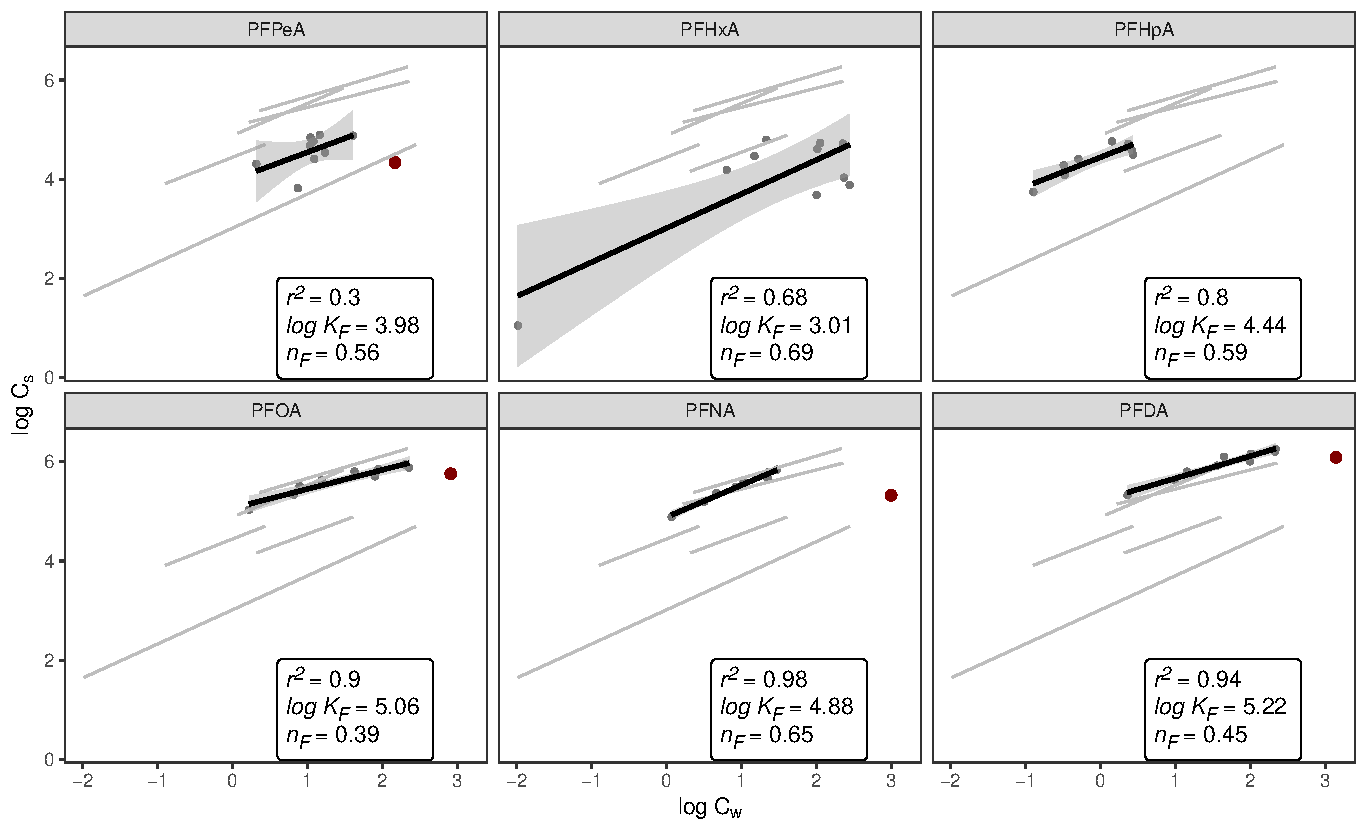
\includegraphics[width=\textwidth]{R/figs/CWC_facet_isotherm.pdf}
    \caption{Freundlich isotherms of TCs in CWC batch tests. Lines are obtained by linear regression.}
    \label{fig:CWC_isotherm2}
\end{figure}

\begin{figure}
    \centering
    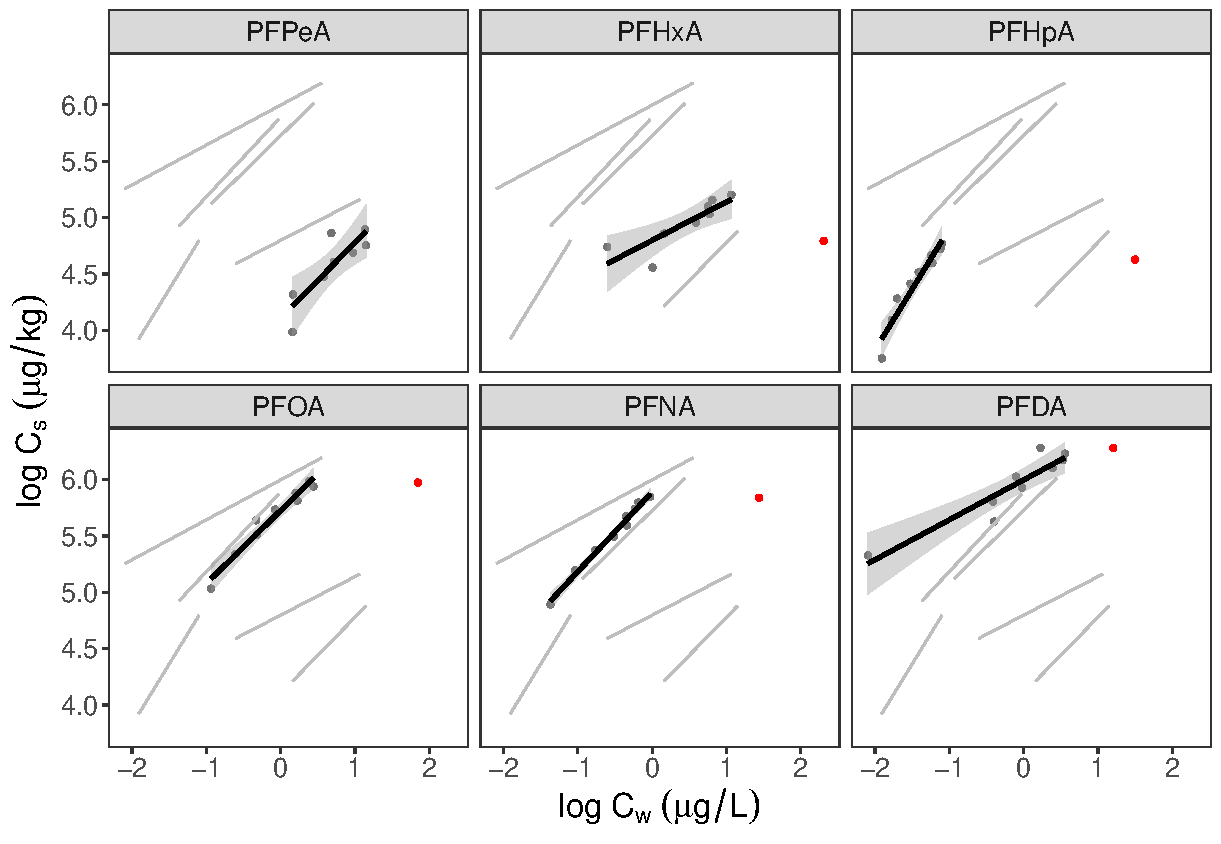
\includegraphics[width=\textwidth]{R/figs/ULS_facet_isotherm.pdf}
    \caption{Freundlich isotherms of TCs in ULS batch tests. Lines are obtained by linear regression.}
    \label{fig:ULS_isotherm2}
\end{figure}

\begin{figure}
    \centering
    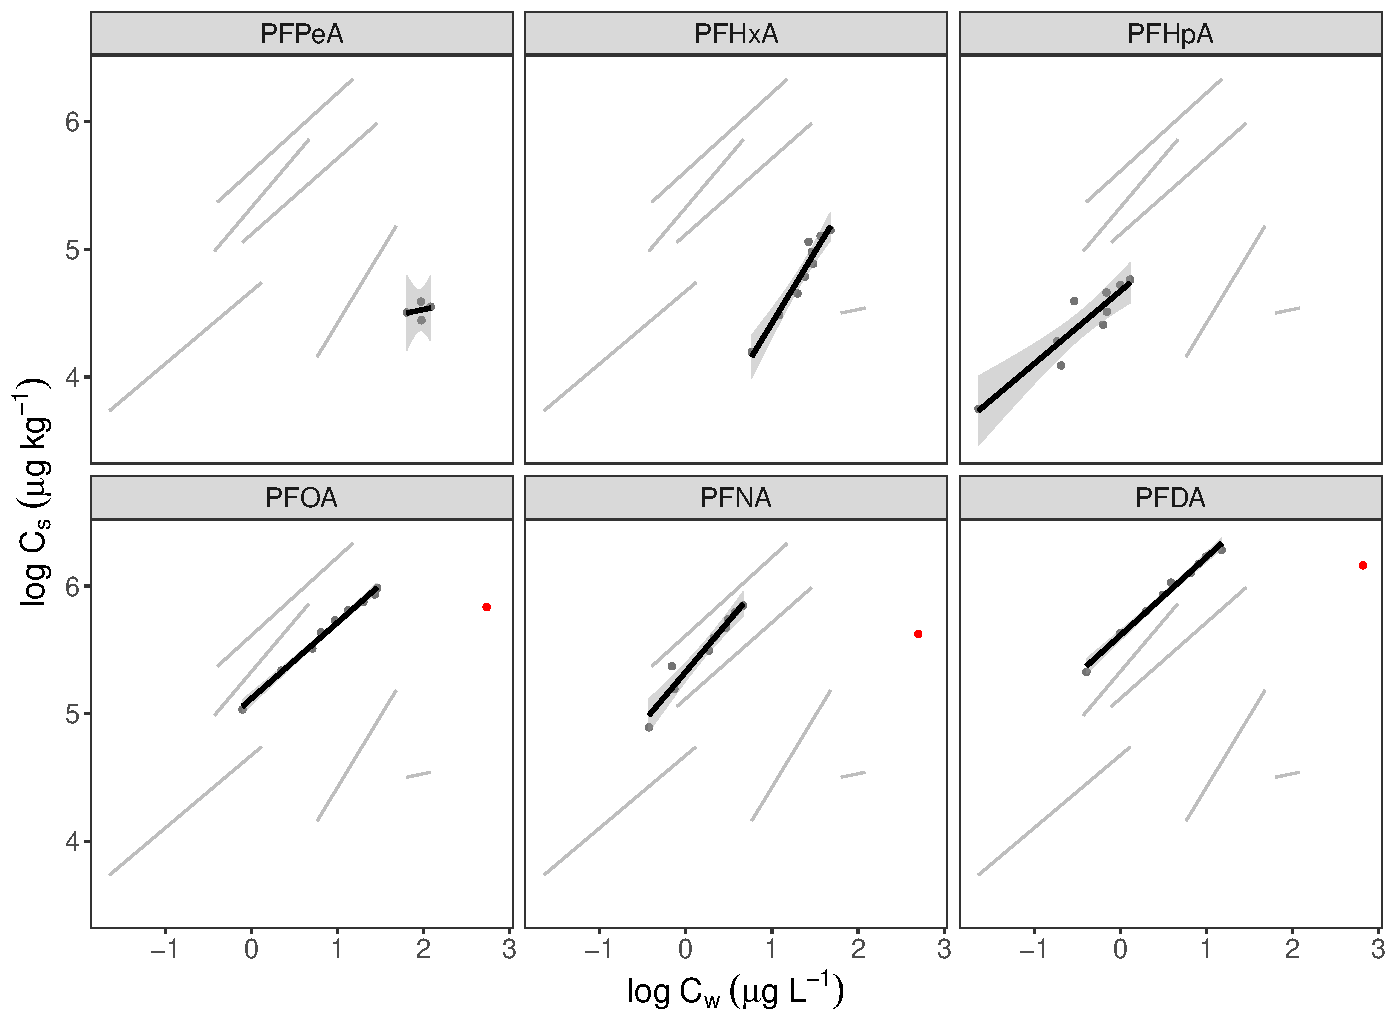
\includegraphics[width=\textwidth]{R/figs/DSL_facet_isotherm.pdf}
    \caption{Freundlich isotherms of TCs in DSL batch tests. Lines are obtained by linear regression.}
    \label{fig:DSL_isotherm2}
\end{figure}

\begin{figure}[tb]
    \centering
    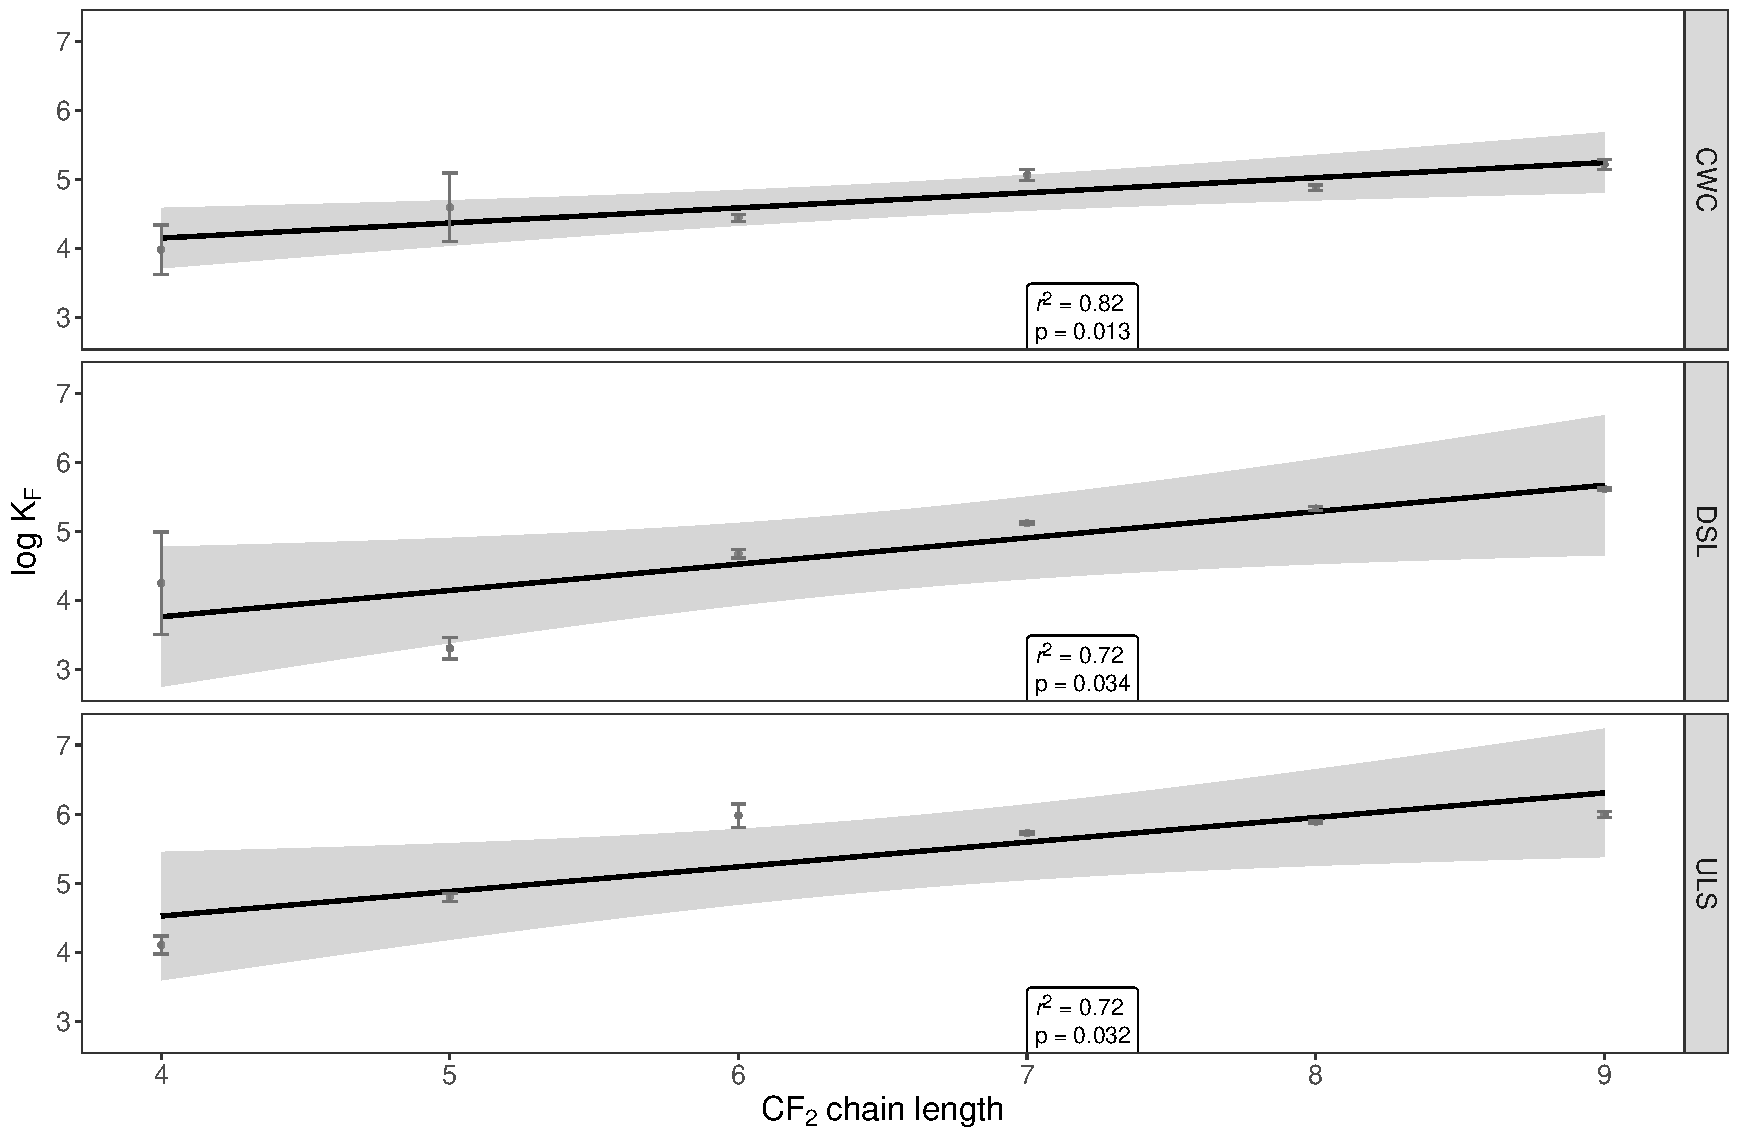
\includegraphics[width=0.7\textwidth]{R/figs/chainlength_KF.pdf}
    \caption{Correlation plot of $log~K_F$ as a function of PFCA chain length (number of $CF_2$ moieties) for the different biochars fitted by linear regression. The error bars and gray area represent the standard error for each $log~K_F$ and the regression line, respectively (n=9).}
    \label{fig:chainlength}
\end{figure}

\begin{figure*}[t!]
    \centering
    \begin{subfigure}[t]{0.5\textwidth}
        \centering
        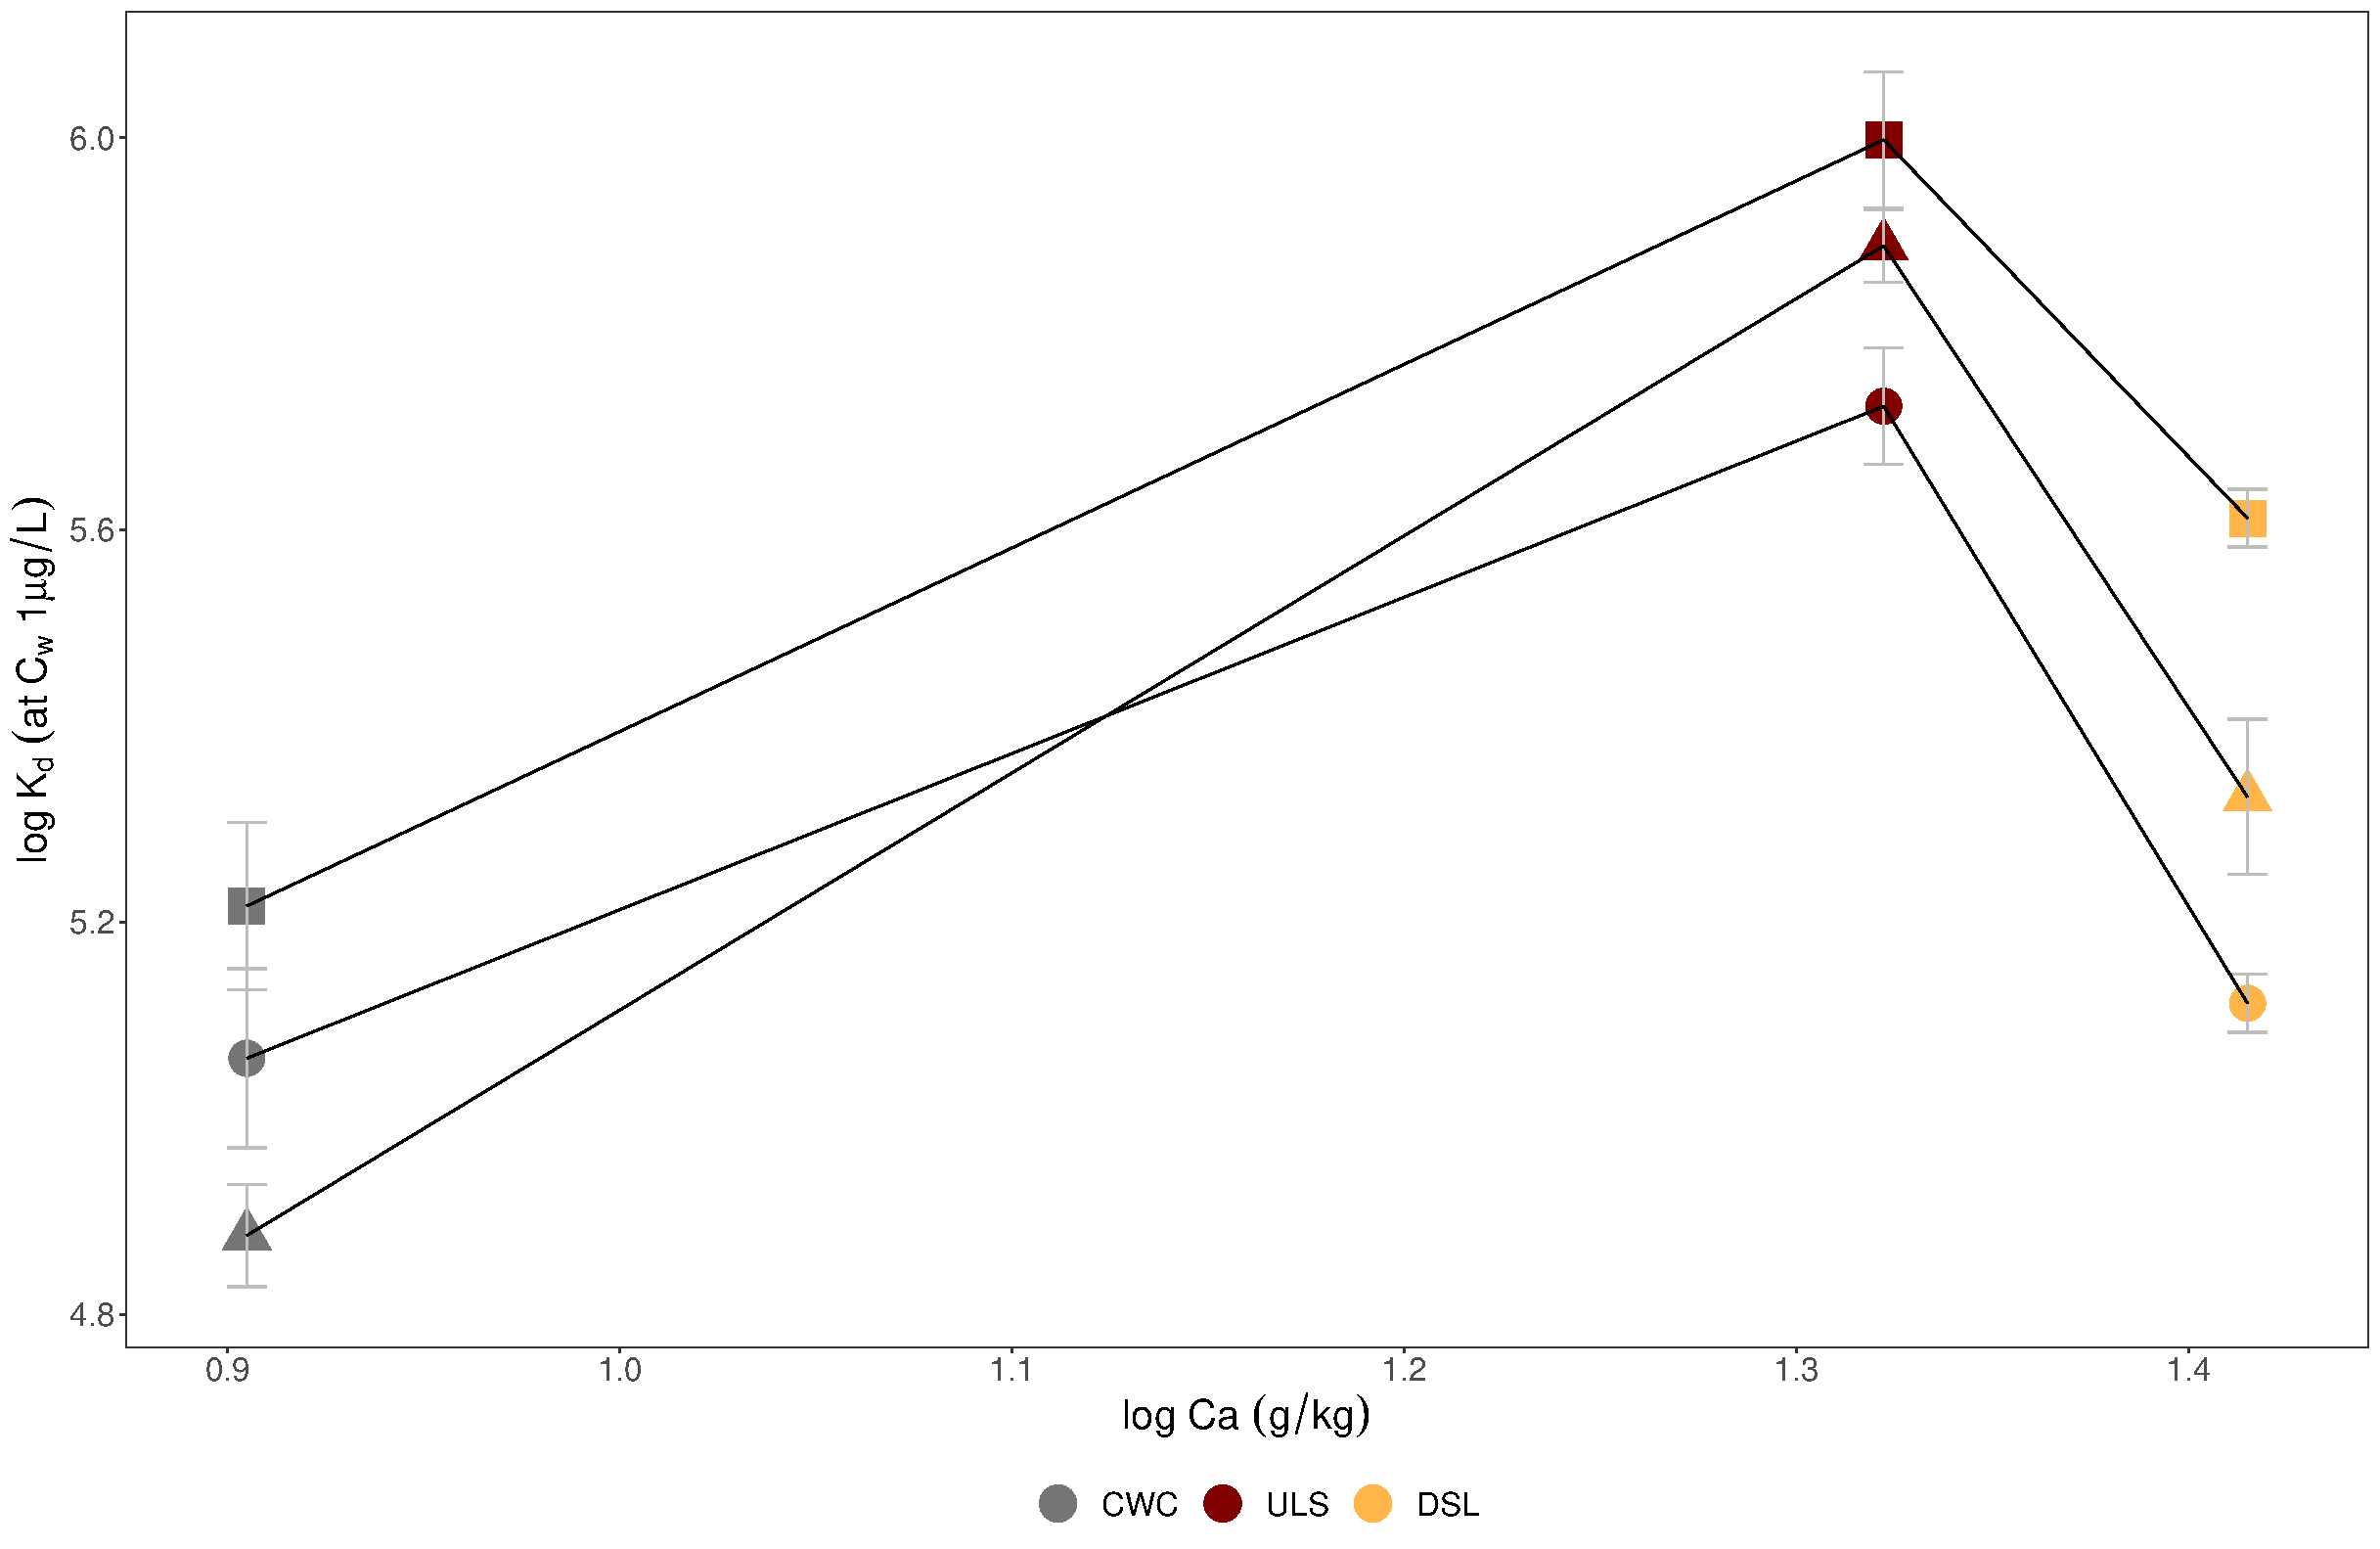
\includegraphics[height=6cm]{R/figs/Kd_1ugL_Ca.pdf}
        \caption{}
        \label{subfig:Ca}
    \end{subfigure}%
    ~ 
    \begin{subfigure}[t]{0.5\textwidth}
        \centering
        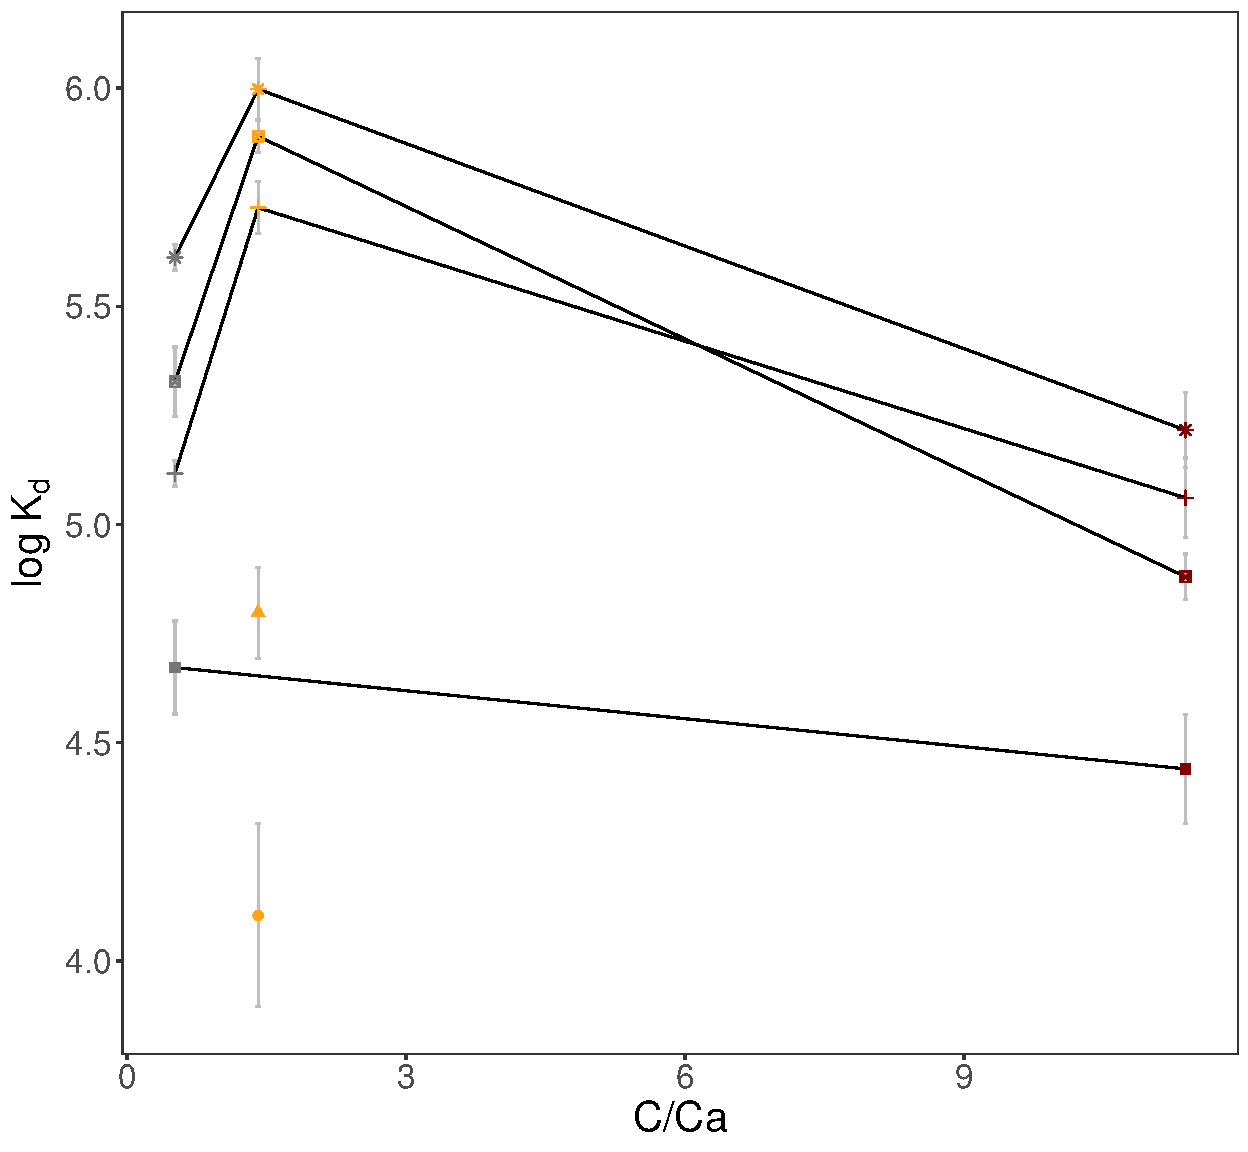
\includegraphics[height=6cm]{R/figs/Kd_1ugL_C_Ca.pdf}
        \caption{}
        \label{subfig:C_Ca}
    \end{subfigure}
    \medskip
    \begin{subfigure}[t]{0.5\textwidth}
        \centering
        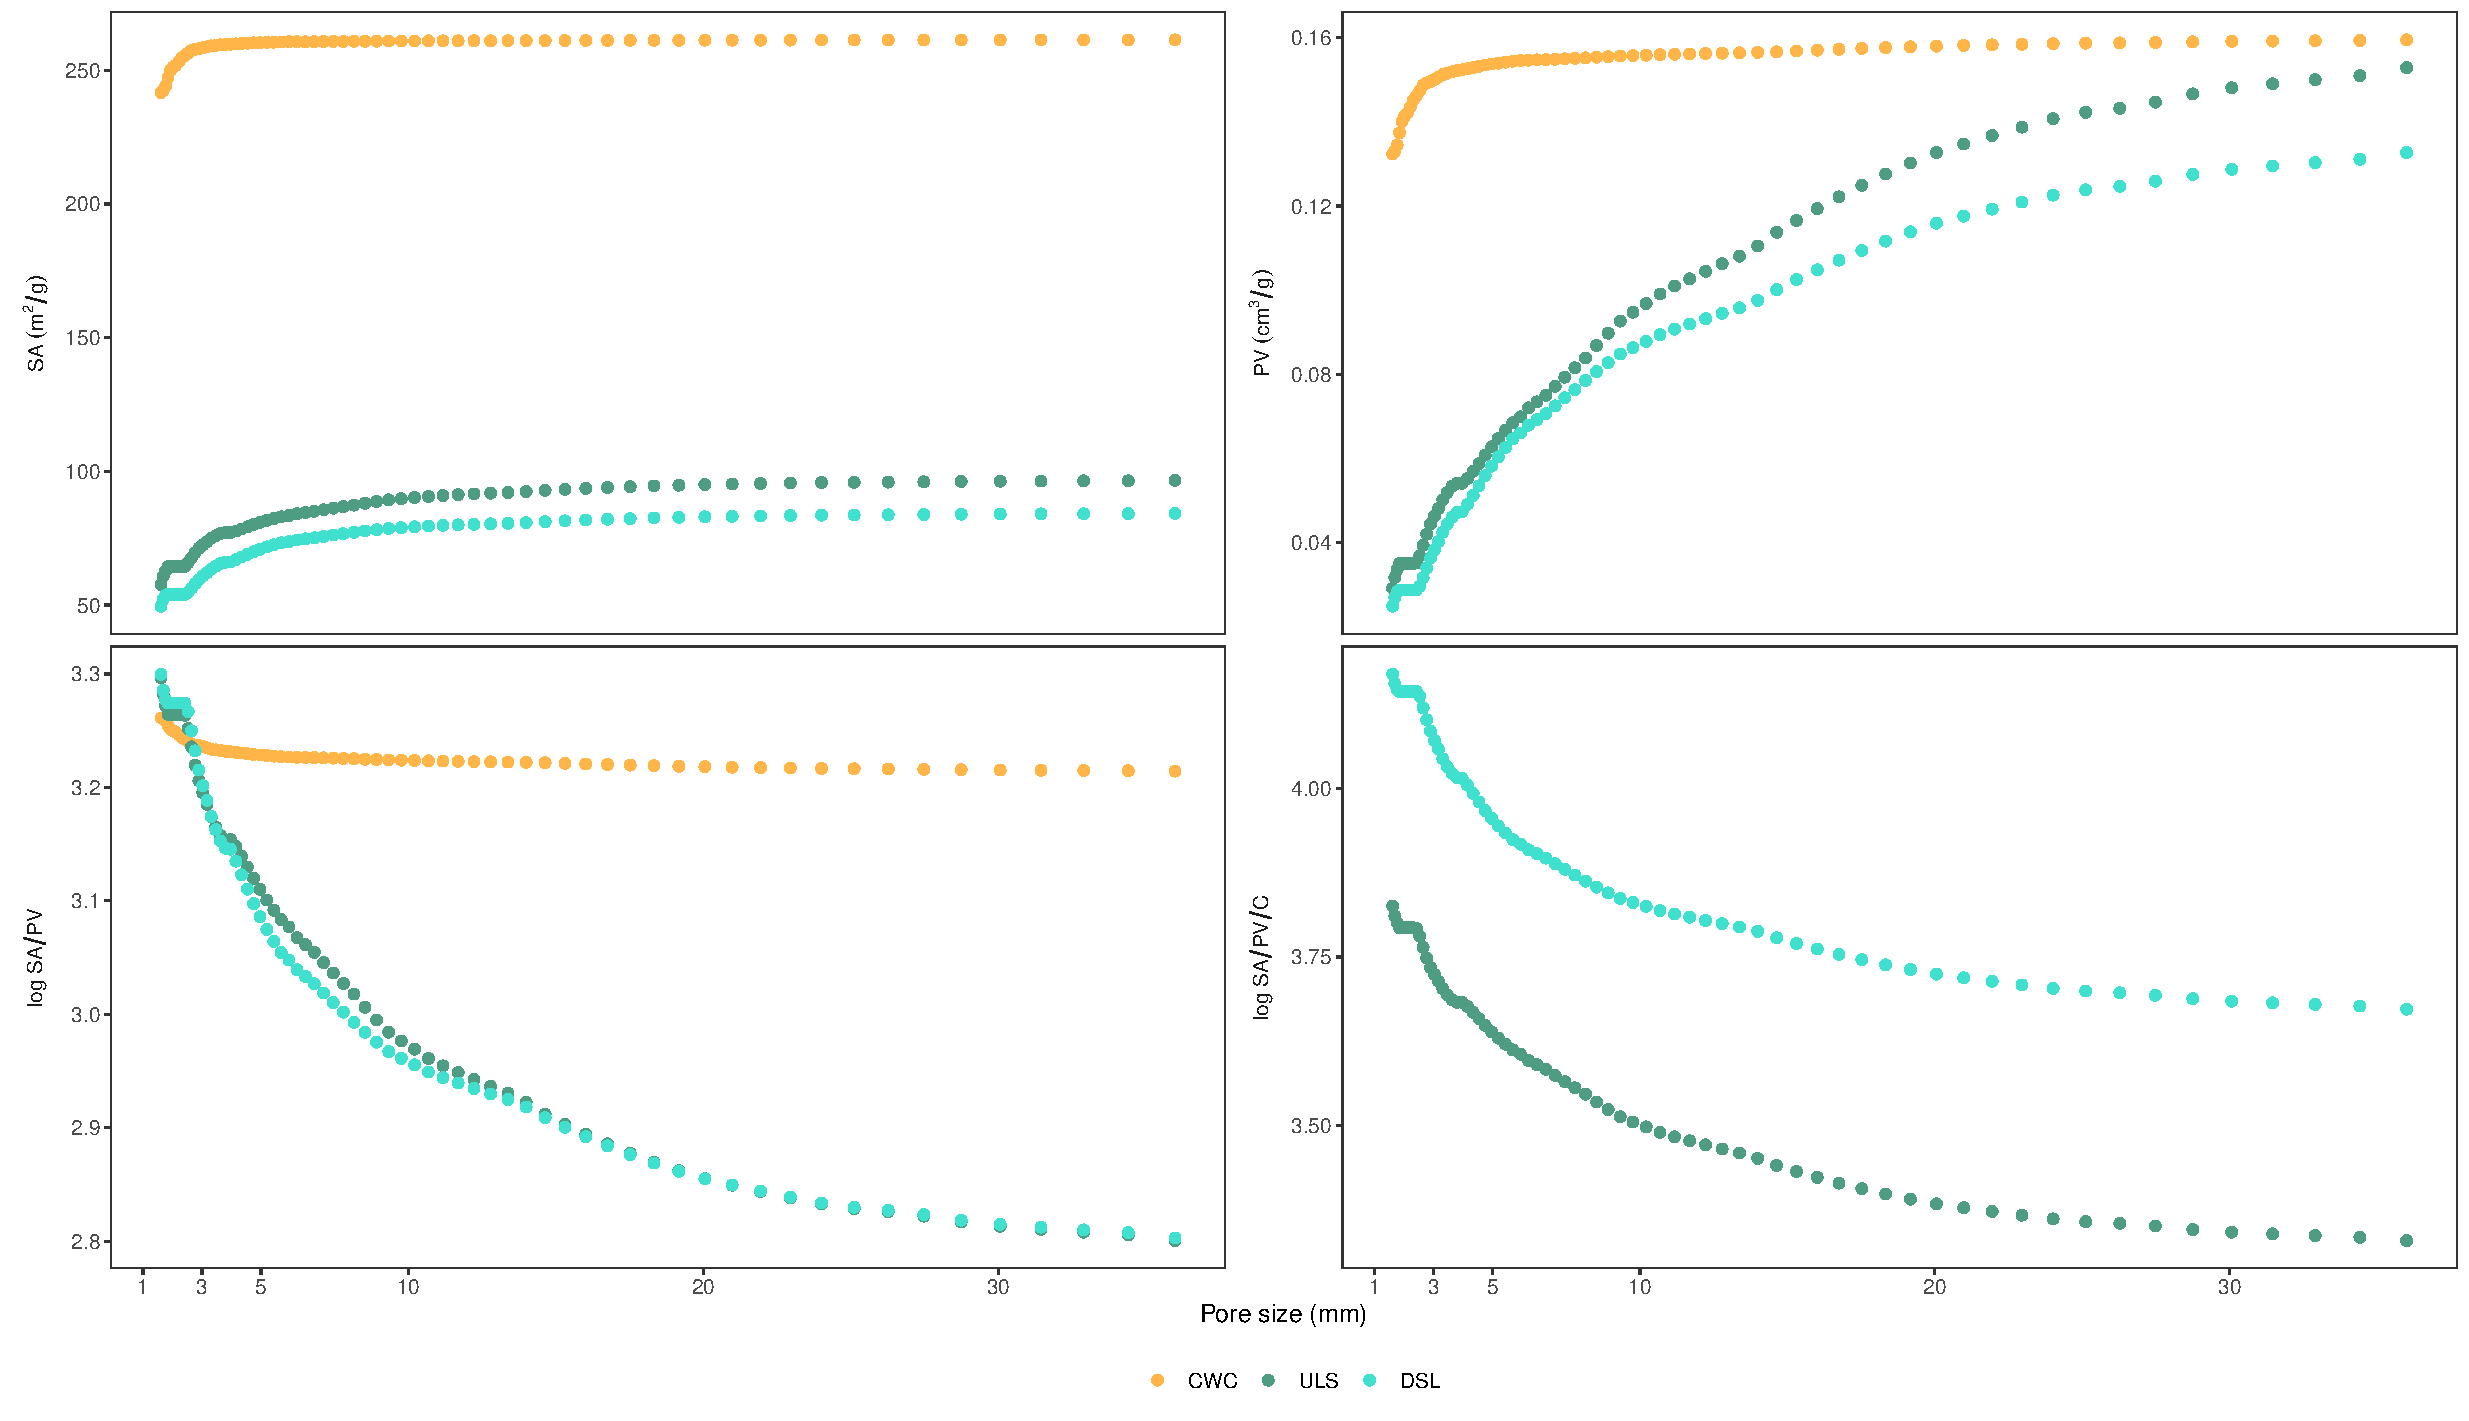
\includegraphics[height=6cm]{R/figs/Kd_1ugL_Fe.pdf}
        \caption{}
        \label{subfig:Fe}
    \end{subfigure}%
    ~ 
    \begin{subfigure}[t]{0.5\textwidth}
        \centering
        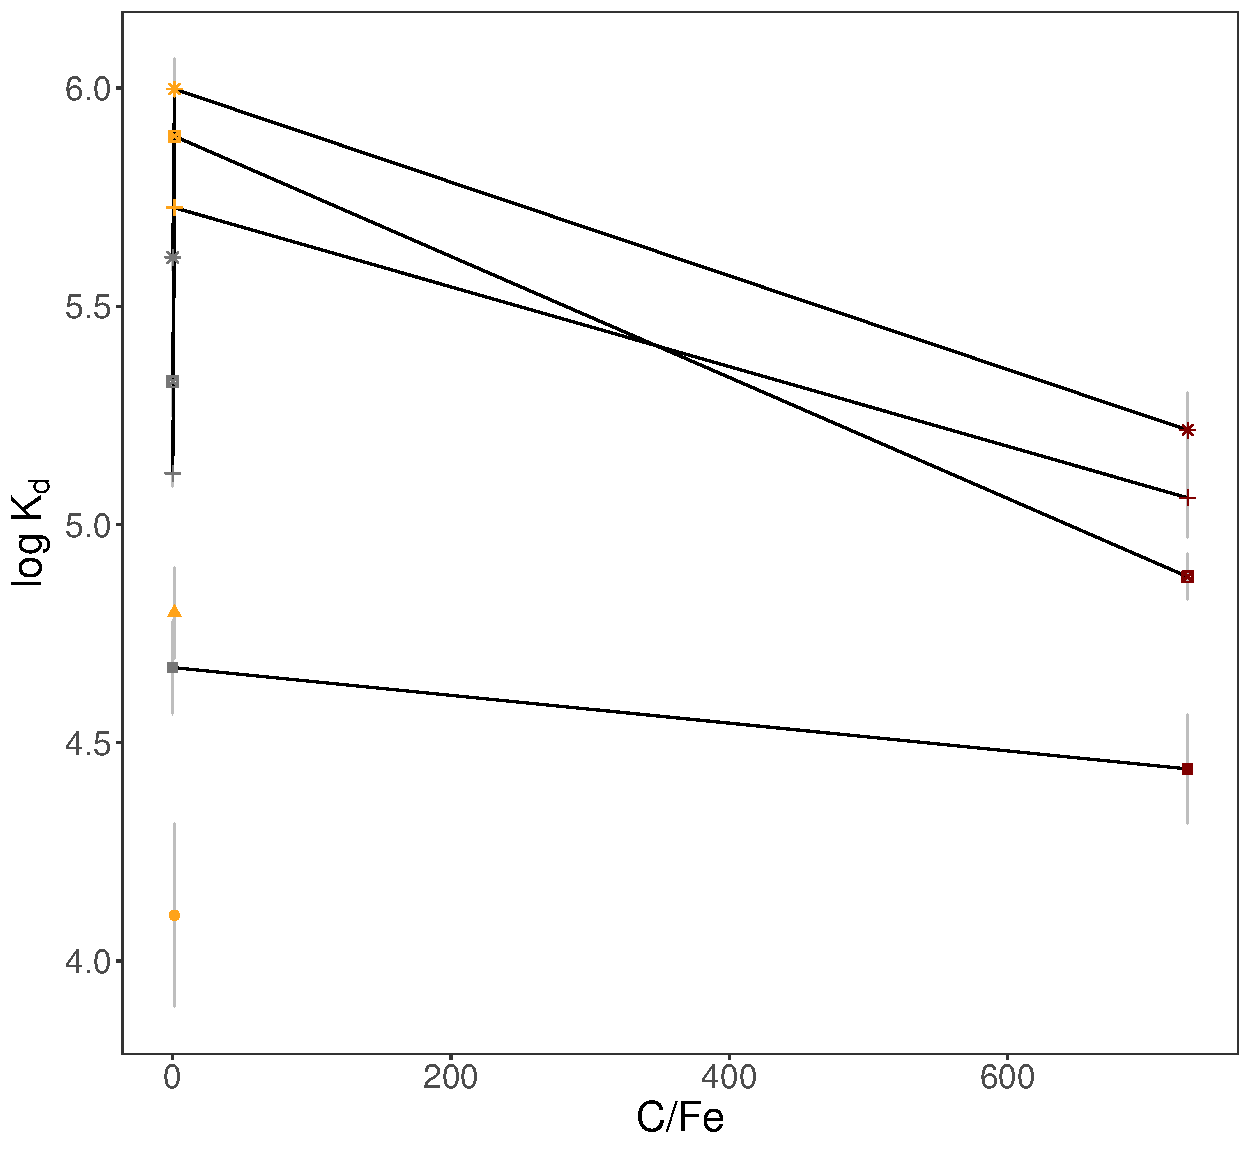
\includegraphics[height=6cm]{R/figs/Kd_1ugL_C_Fe.pdf}
        \caption{}
        \label{subfig:C_Fe}
    \end{subfigure}
    \label{fig:C_Ca_Fe}
    \caption{}
\end{figure*}

\begin{table}
\centering
\caption{Correlation table $log~K_d$ normalized to 1 \textmu g L\textsuperscript{-1} $C_w$.}
\label{tab:correlation}
\adjustbox{max width=\textwidth}{
\begin{tabular}{lrrrrrrrrrrrrrrrrrr} \toprule
PFCA & \multicolumn{2}{c}{Ca} & \multicolumn{2}{c}{Fe} & \multicolumn{2}{c}{C} & \multicolumn{2}{c}{C/Ca} & \multicolumn{2}{c}{C/Fe} & \multicolumn{2}{c}{SA small} & \multicolumn{2}{c}{PV small} & \multicolumn{2}{c}{SA large} & \multicolumn{2}{c}{PV large} \\ \cmidrule(l){2-3} \cmidrule(l){4-5} \cmidrule(l){6-7} \cmidrule(l){8-9} \cmidrule(l){10-11} \cmidrule(l){12-13} \cmidrule(l){14-15} \cmidrule(l){16-17} \cmidrule(l){18-19}
 & \multicolumn{1}{c}{$r^2$} & \multicolumn{1}{c}{$p$} & \multicolumn{1}{c}{$r^2$} & \multicolumn{1}{c}{$p$} & \multicolumn{1}{c}{$r^2$} & \multicolumn{1}{c}{$p$} & \multicolumn{1}{c}{$r^2$} & \multicolumn{1}{c}{$p$} & \multicolumn{1}{c}{$r^2$} & \multicolumn{1}{c}{$p$} & \multicolumn{1}{c}{$r^2$} & \multicolumn{1}{c}{$p$} & \multicolumn{1}{c}{$r^2$} & \multicolumn{1}{c}{$p$} & \multicolumn{1}{c}{$r^2$} & \multicolumn{1}{c}{$p$} & \multicolumn{1}{c}{$r^2$} & \multicolumn{1}{c}{$p$} \\ \midrule
PFPeA & 0.92 & 0.19 & 0.87 & 0.23 & 0.87 & 0.23 & 0.77 & 0.31 & 0.71 & 0.36 & 0.81 & 0.28 & 0.81 & 0.29 & 0.78 & 0.31 & 0.59 & 0.44 \\
PFHxA & 0.1 & 0.79 & 0.1 & 0.79 & 0.15 & 0.74 & 0.25 & 0.66 & 0.32 & 0.62 & 0.21 & 0.69 & 0.22 & 0.69 & 0.25 & 0.67 & 0.44 & 0.54 \\
PFHpA & 0.15 & 0.75 & 0.069 & 0.83 & 0.2 & 0.7 & 0.31 & 0.62 & 0.38 & 0.58 & 0.27 & 0.65 & 0.27 & 0.65 & 0.31 & 0.63 & 0.51 & 0.5 \\
PFOA & 0.1 & 0.79 & 0.11 & 0.79 & 0.15 & 0.74 & 0.25 & 0.67 & 0.32 & 0.62 & 0.21 & 0.7 & 0.22 & 0.69 & 0.25 & 0.67 & 0.44 & 0.54 \\
PFNA & 0.42 & 0.55 & 0.0026 & 0.97 & 0.5 & 0.5 & 0.62 & 0.42 & 0.69 & 0.38 & 0.58 & 0.45 & 0.58 & 0.45 & 0.62 & 0.42 & 0.8 & 0.29 \\
PFDA & 0.5 & 0.5 & 0.015 & 0.92 & 0.57 & 0.45 & 0.69 & 0.38 & 0.75 & 0.33 & 0.65 & 0.41 & 0.65 & 0.4 & 0.69 & 0.38 & 0.86 & 0.25 \\
 &  &  &  &  &  &  &  &  &  &  &  &  &  &  &  &  &  &  \\ \midrule
PFCA & \multicolumn{2}{c}{SA large/Fe} & \multicolumn{2}{c}{SA large/Ca} & \multicolumn{2}{c}{SA small/Fe} & \multicolumn{2}{c}{SA small/Ca} & \multicolumn{2}{c}{PV large/Fe} & \multicolumn{2}{c}{PV large/Ca} & \multicolumn{2}{c}{PV small/Fe} & \multicolumn{2}{c}{PV small/Ca} &  &  \\ \cmidrule(l){2-3} \cmidrule(l){4-5} \cmidrule(l){6-7} \cmidrule(l){8-9} \cmidrule(l){10-11} \cmidrule(l){12-13} \cmidrule(l){14-15} \cmidrule(l){16-17}
 & \multicolumn{1}{c}{$r^2$} & \multicolumn{1}{c}{$p$} & \multicolumn{1}{c}{$r^2$} & \multicolumn{1}{c}{$p$} & \multicolumn{1}{c}{$r^2$} & \multicolumn{1}{c}{$p$} & \multicolumn{1}{c}{$r^2$} & \multicolumn{1}{c}{$p$} & \multicolumn{1}{c}{$r^2$} & \multicolumn{1}{c}{$p$} & \multicolumn{1}{c}{$r^2$} & \multicolumn{1}{c}{$p$} & \multicolumn{1}{c}{$r^2$} & \multicolumn{1}{c}{$p$} & \multicolumn{1}{c}{$r^2$} & \multicolumn{1}{c}{$p$} &  &  \\ \midrule
PFPeA & 0.71 & 0.36 & 0.75 & 0.33 & 0.71 & 0.36 & 0.75 & 0.33 & 0.74 & 0.34 & 0.27 & 0.65 & 0.71 & 0.36 & 0.75 & 0.33 &  &  \\
PFHxA & 0.32 & 0.62 & 0.28 & 0.65 & 0.32 & 0.62 & 0.27 & 0.65 & 0.29 & 0.64 & 0.76 & 0.32 & 0.32 & 0.62 & 0.28 & 0.65 &  &  \\
PFHpA & 0.38 & 0.58 & 0.34 & 0.61 & 0.38 & 0.58 & 0.33 & 0.61 & 0.35 & 0.6 & 0.81 & 0.28 & 0.38 & 0.58 & 0.33 & 0.61 &  &  \\
PFOA & 0.32 & 0.62 & 0.28 & 0.65 & 0.32 & 0.62 & 0.27 & 0.65 & 0.29 & 0.64 & 0.76 & 0.32 & 0.32 & 0.62 & 0.27 & 0.65 &  &  \\
PFNA & 0.69 & 0.38 & 0.65 & 0.41 & 0.69 & 0.38 & 0.65 & 0.41 & 0.66 & 0.4 & 0.98 & 0.082 & 0.69 & 0.38 & 0.65 & 0.41 &  &  \\
PFDA & 0.75 & 0.33 & 0.72 & 0.36 & 0.76 & 0.33 & 0.71 & 0.36 & 0.73 & 0.35 & 1 & 0.035 & 0.76 & 0.33 & 0.71 & 0.36 &  & \\ \bottomrule
\end{tabular}}
\end{table}

\begin{figure*}[t!]
    \centering
    \begin{subfigure}[t]{0.5\textwidth}
        \centering
        \includegraphics[height=5cm]{R/figs/Kd_1ugL_SAN2.pdf}
        \caption{}
        \label{subfig:SAN2}
    \end{subfigure}%
    ~ 
    \begin{subfigure}[t]{0.5\textwidth}
        \centering
        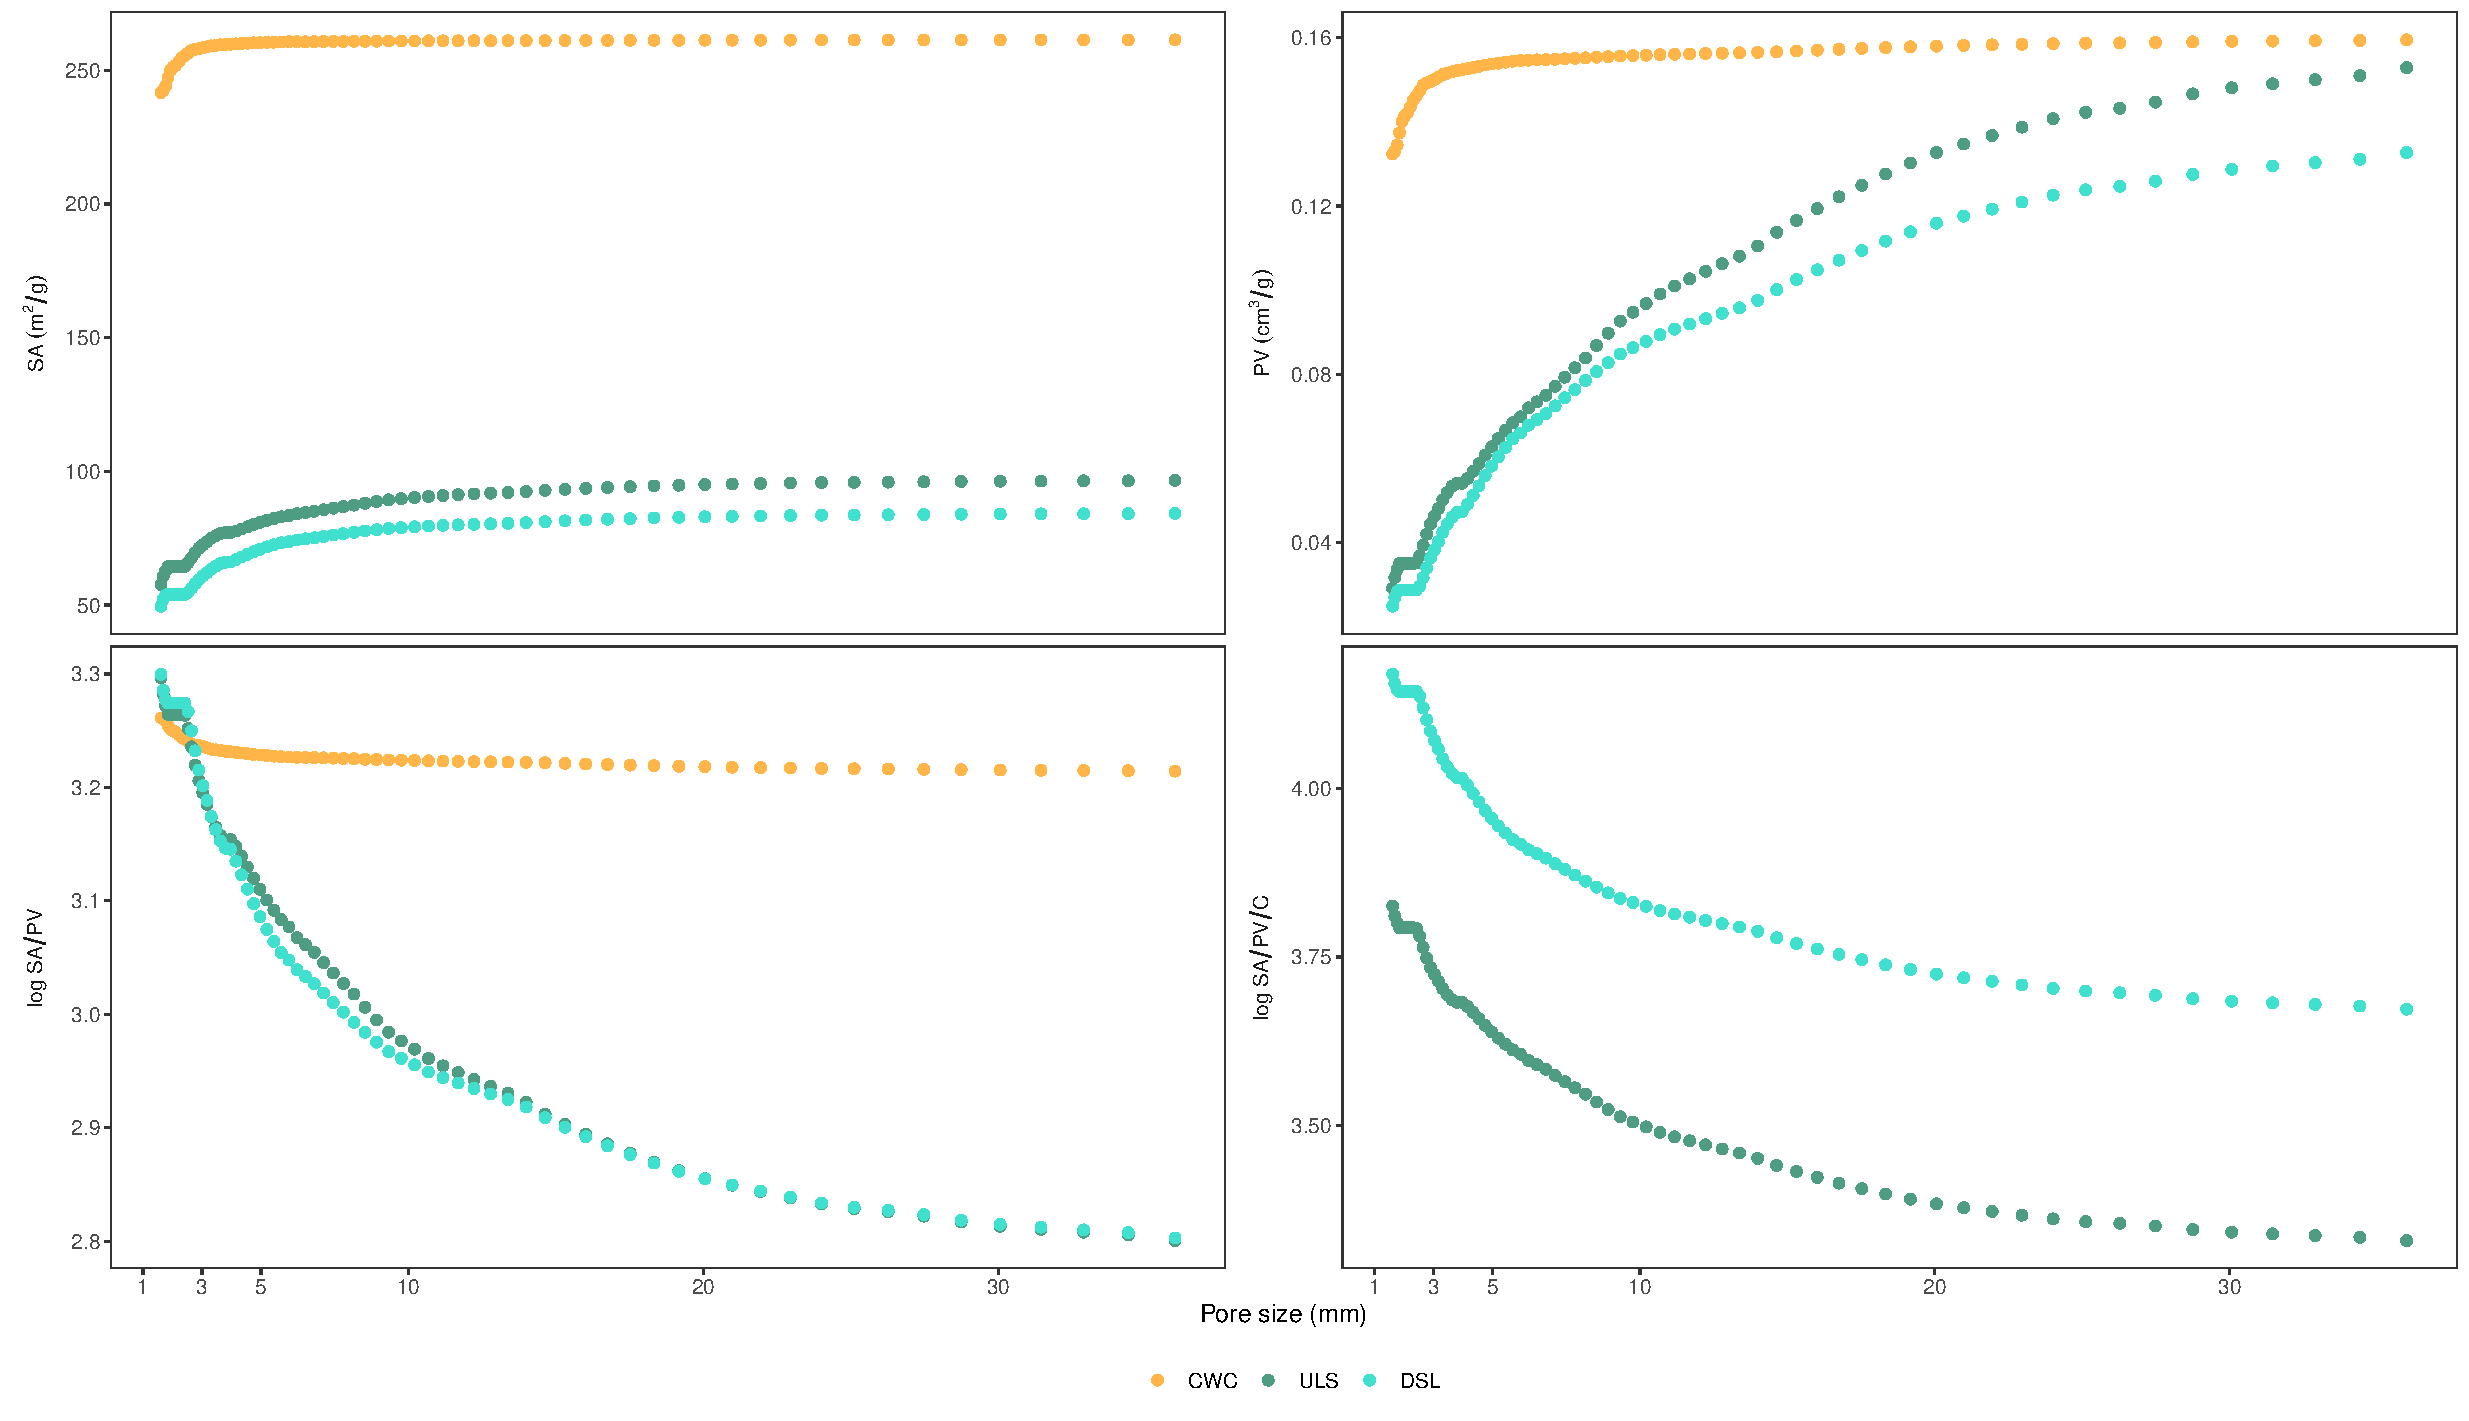
\includegraphics[height=5cm]{R/figs/Kd_1ugL_SACO2.pdf}
        \caption{}
        \label{subfig:SACO2}
    \end{subfigure}
    \medskip
    \begin{subfigure}[t]{0.5\textwidth}
        \centering
        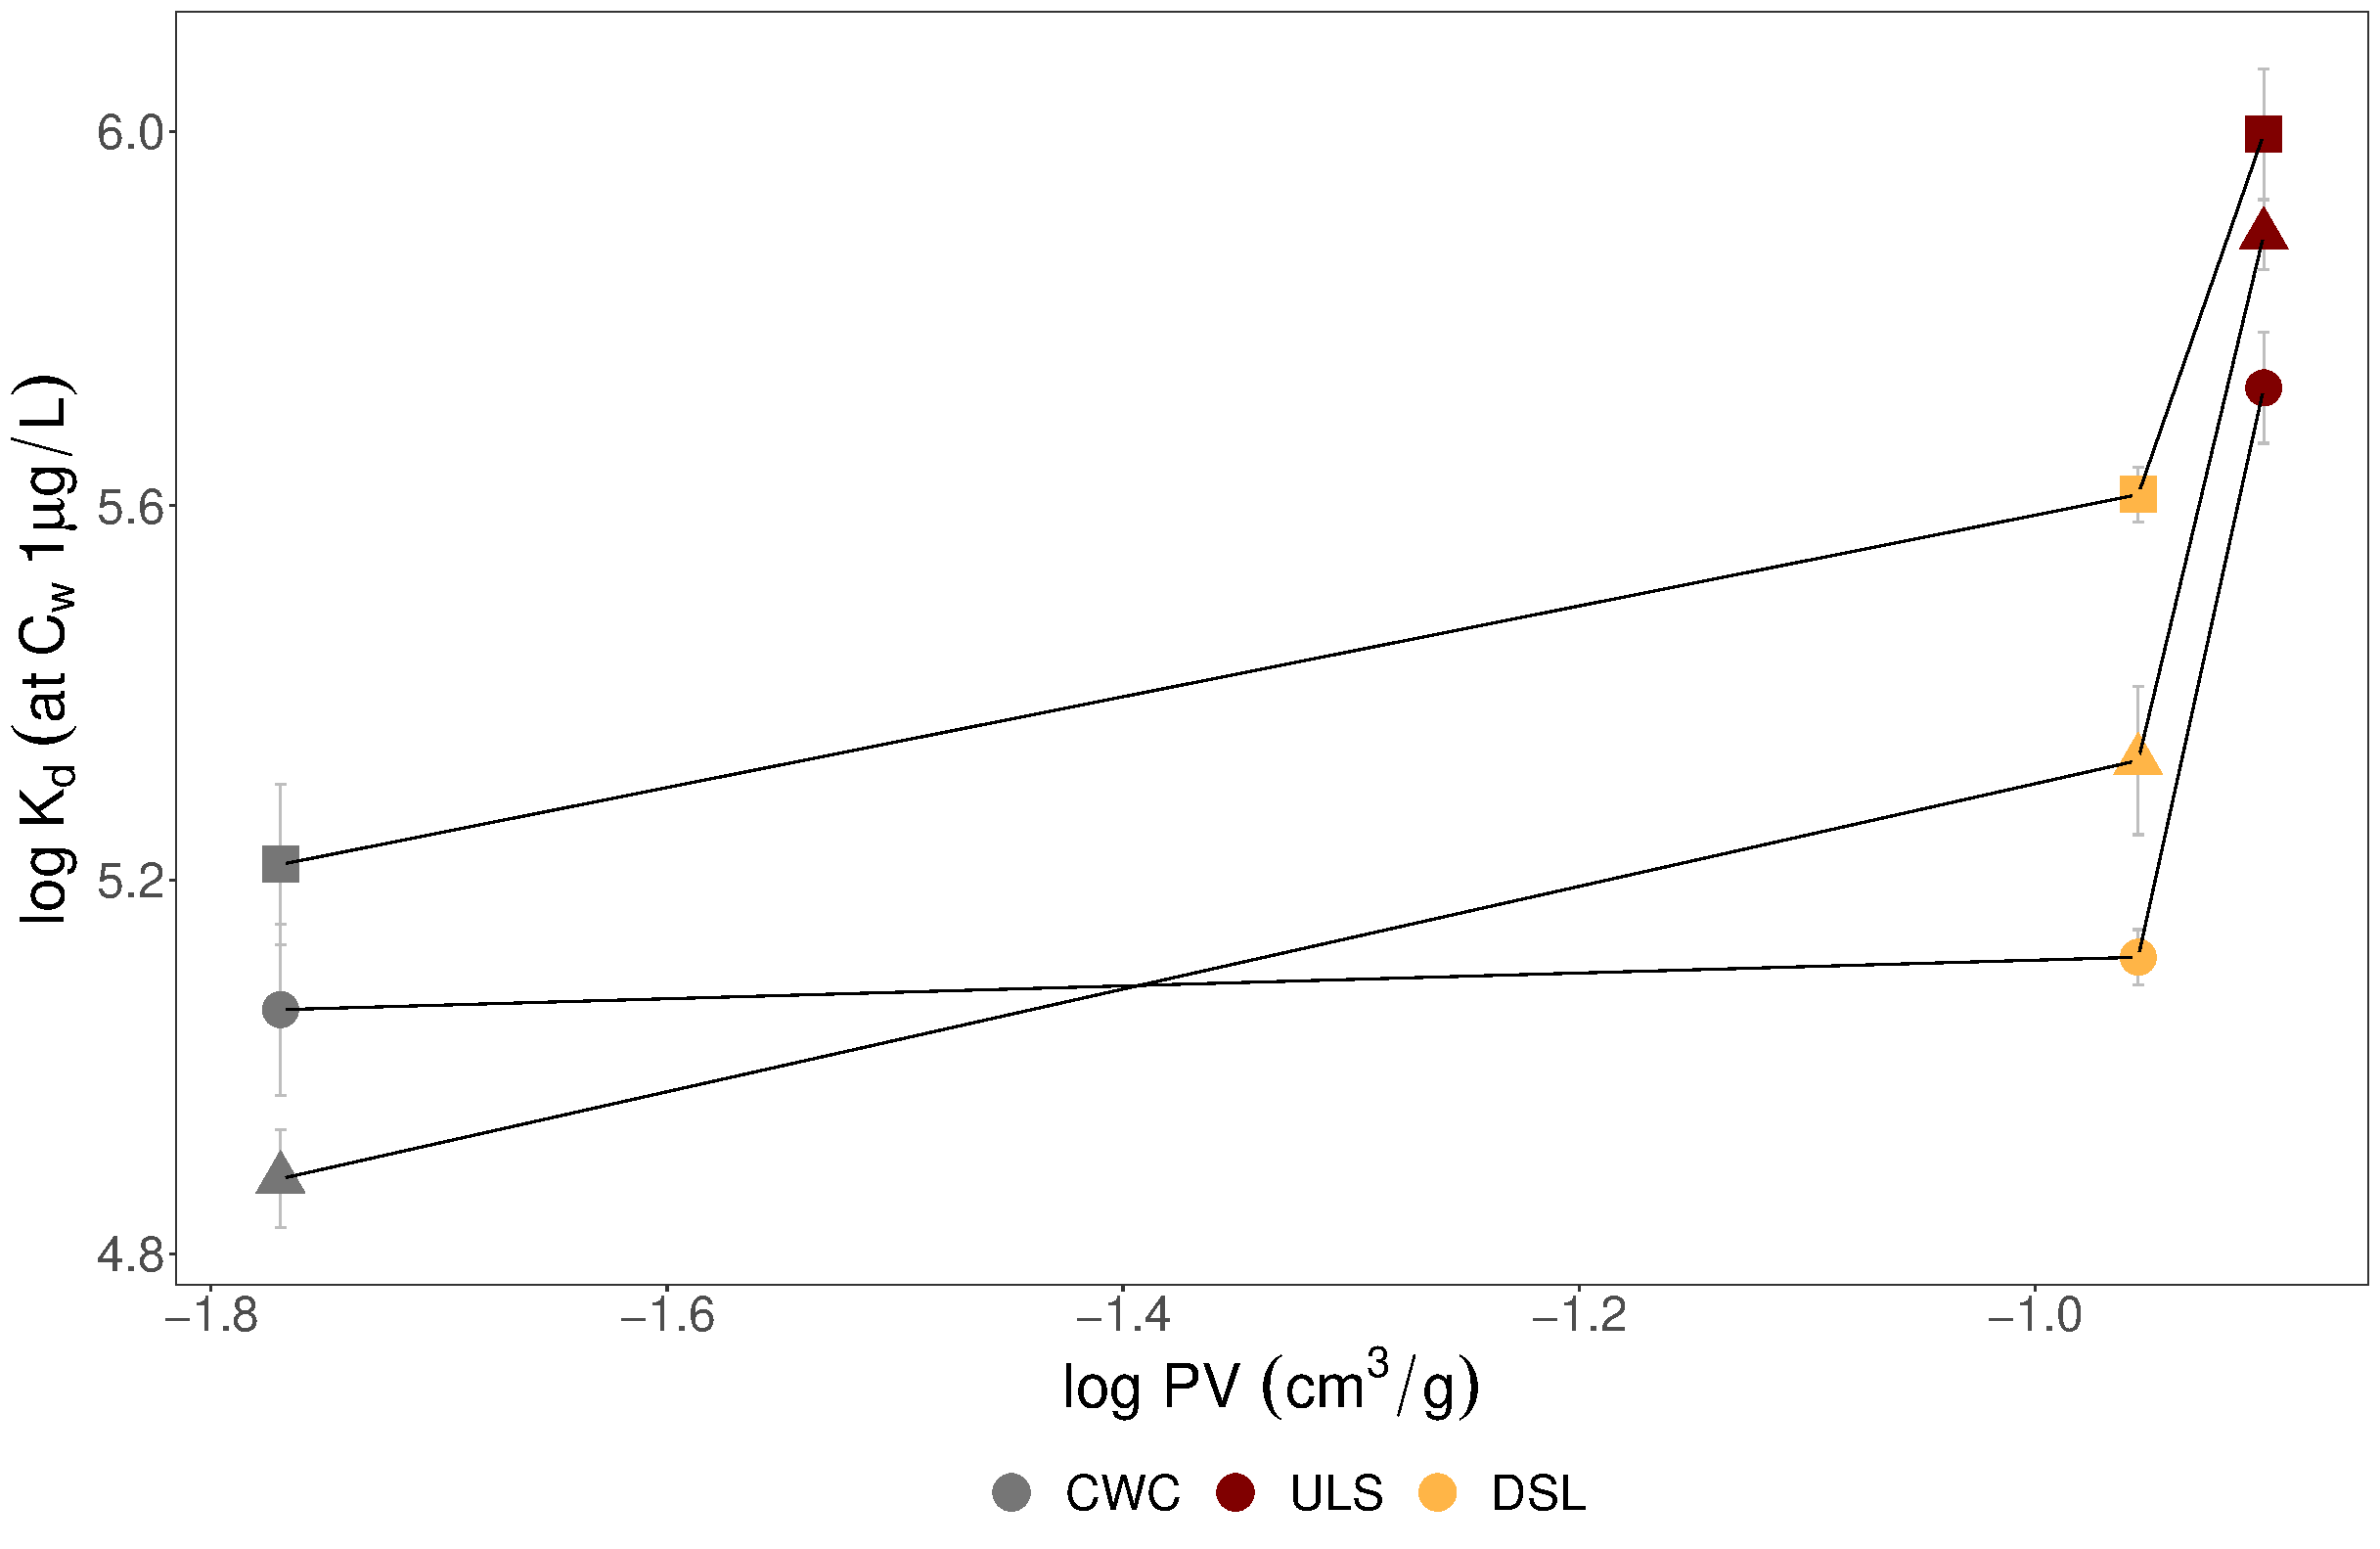
\includegraphics[height=5cm]{R/figs/Kd_1ugL_PVN2.pdf}
        \caption{}
        \label{subfig:PVN2}
    \end{subfigure}%
    ~ 
    \begin{subfigure}[t]{0.5\textwidth}
        \centering
        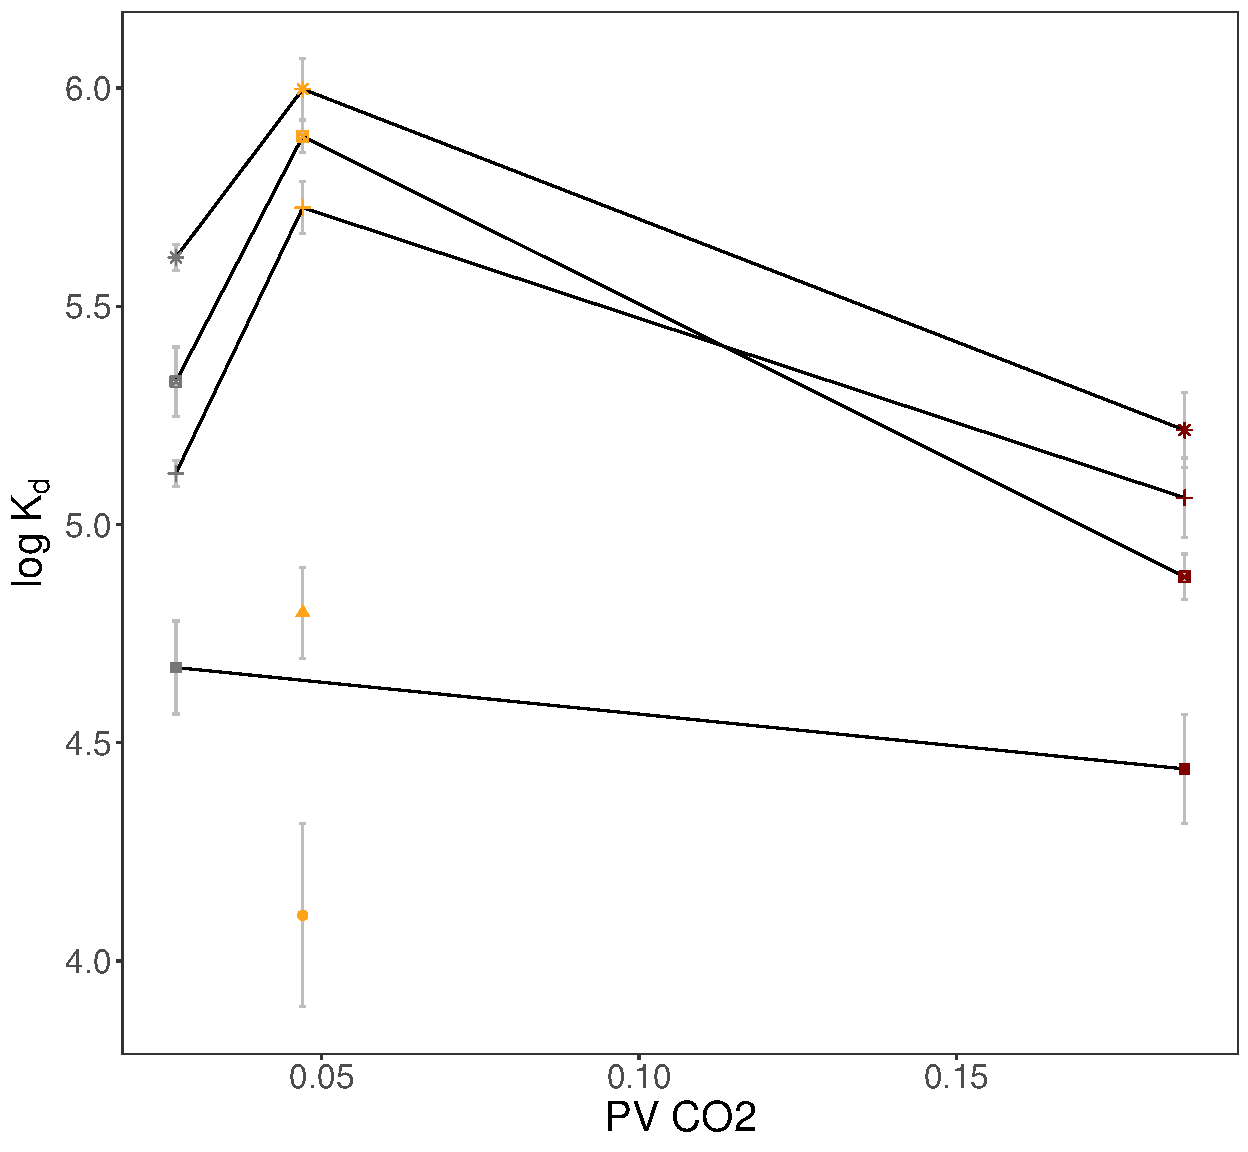
\includegraphics[height=5cm]{R/figs/Kd_1ugL_PVCO2.pdf}
        \caption{}
        \label{subfig:PVCO2}
    \end{subfigure}
    \medskip
    \begin{subfigure}[t]{0.5\textwidth}
        \centering
        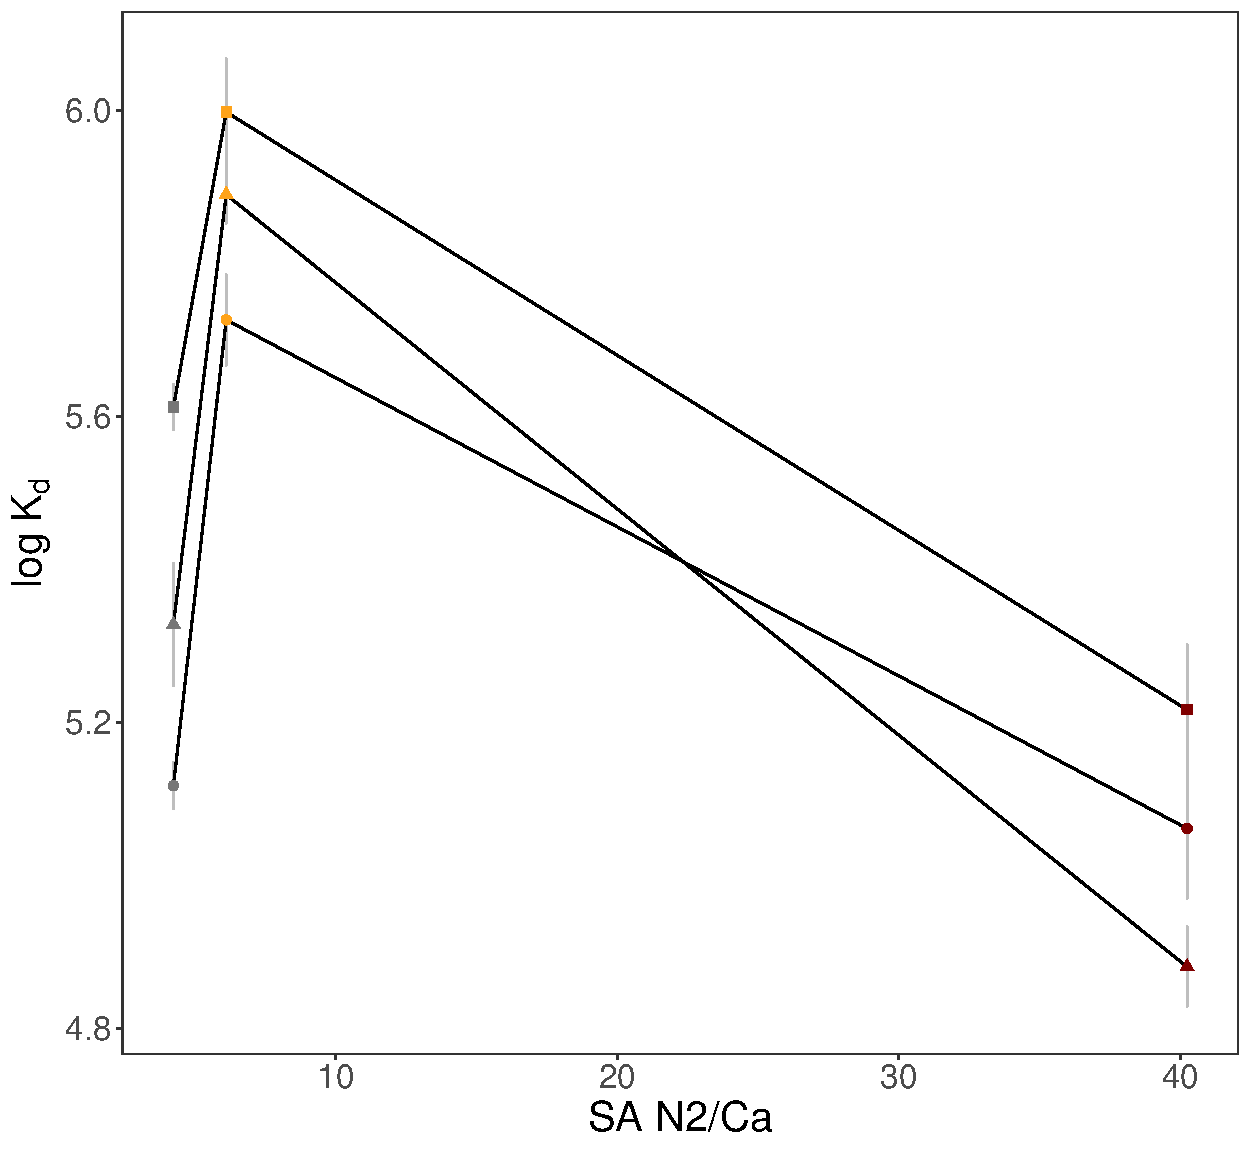
\includegraphics[height=5cm]{R/figs/Kd_1ugL_SAN2_Ca.pdf}
        \caption{}
        \label{subfig:SAN2_Ca}
    \end{subfigure}%
    ~ 
    \begin{subfigure}[t]{0.5\textwidth}
        \centering
        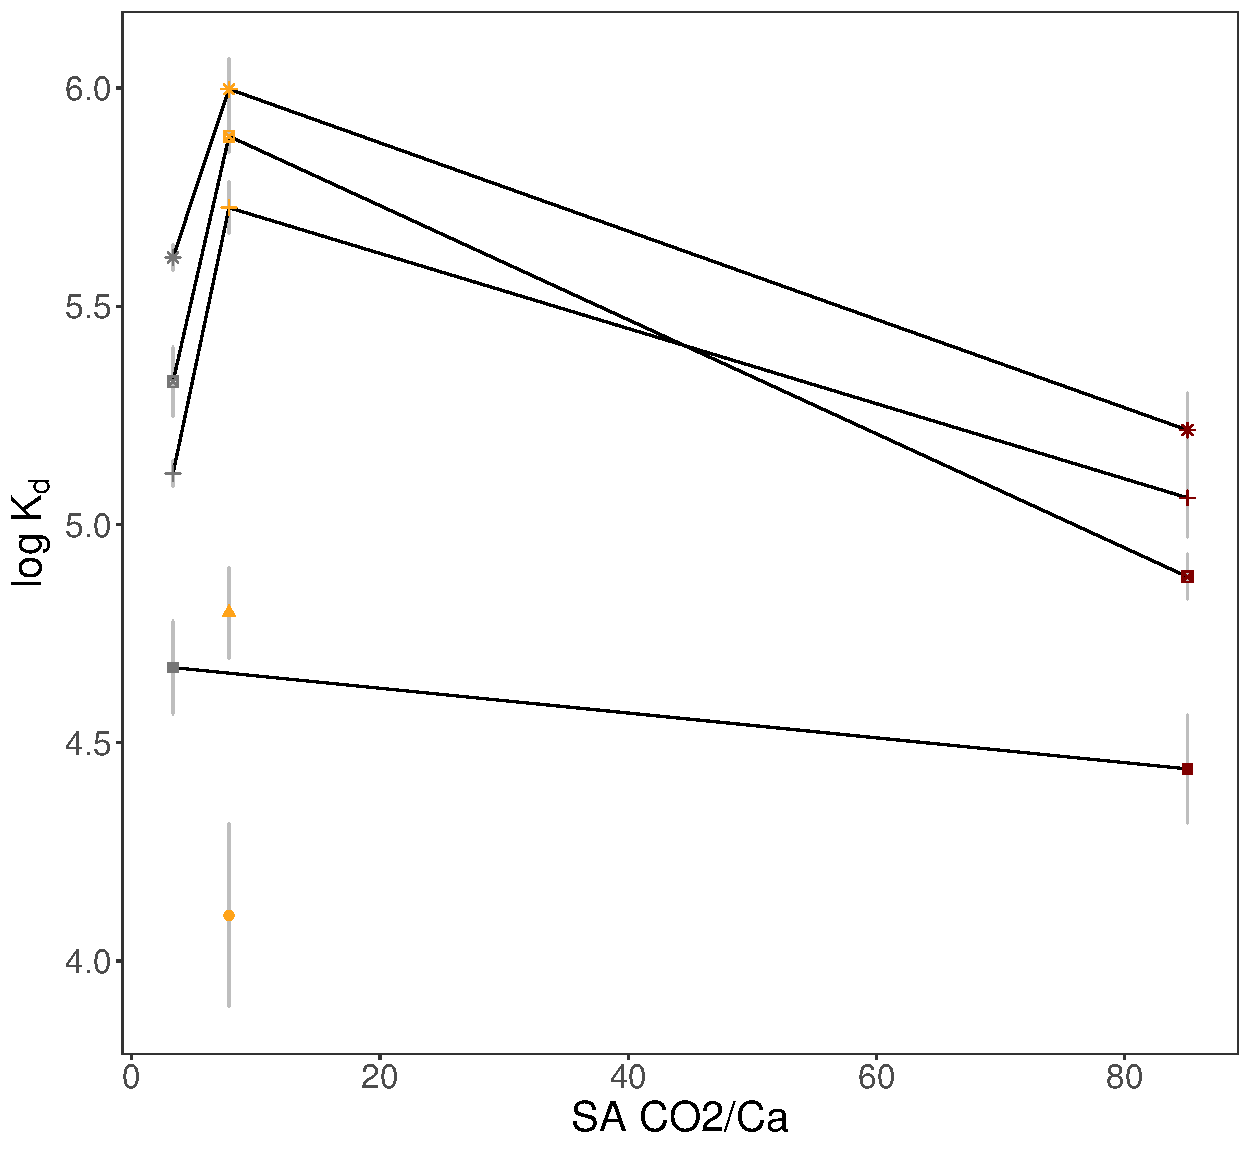
\includegraphics[height=5cm]{R/figs/Kd_1ugL_SACO2_Ca.pdf}
        \caption{}
        \label{subfig:SACO2_Ca}
    \end{subfigure}
    \medskip
    \begin{subfigure}[t]{0.5\textwidth}
        \centering
        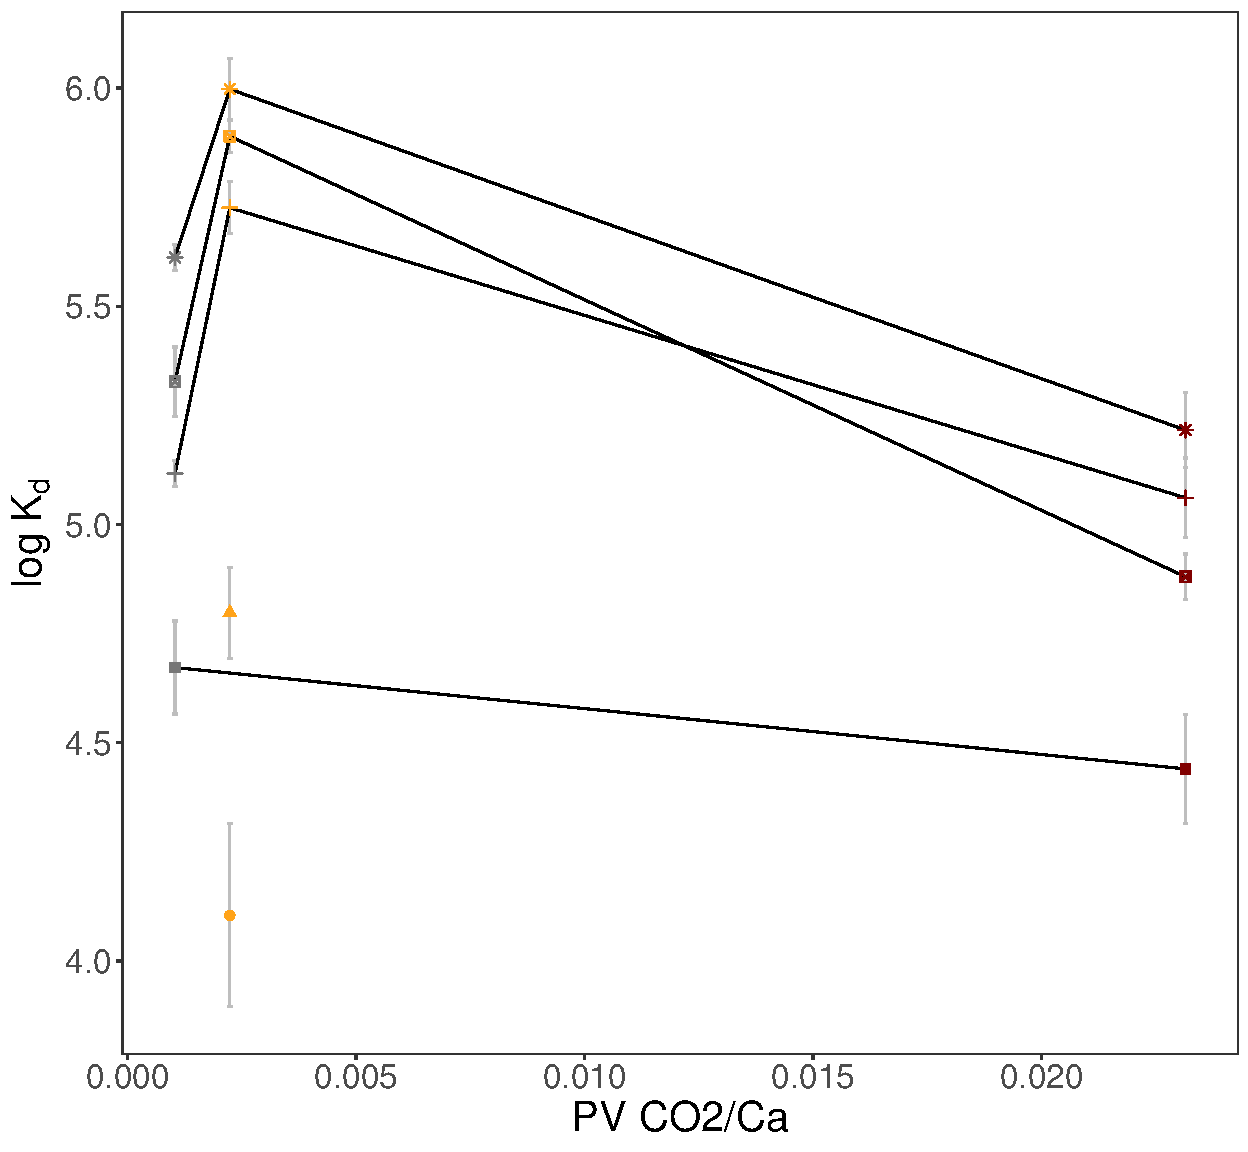
\includegraphics[height=5cm]{R/figs/Kd_1ugL_PVCO2_Ca.pdf}
        \caption{}
        \label{subfig:PVCO2_Ca}
    \end{subfigure}%
    ~ 
    \begin{subfigure}[t]{0.5\textwidth}
        \centering
        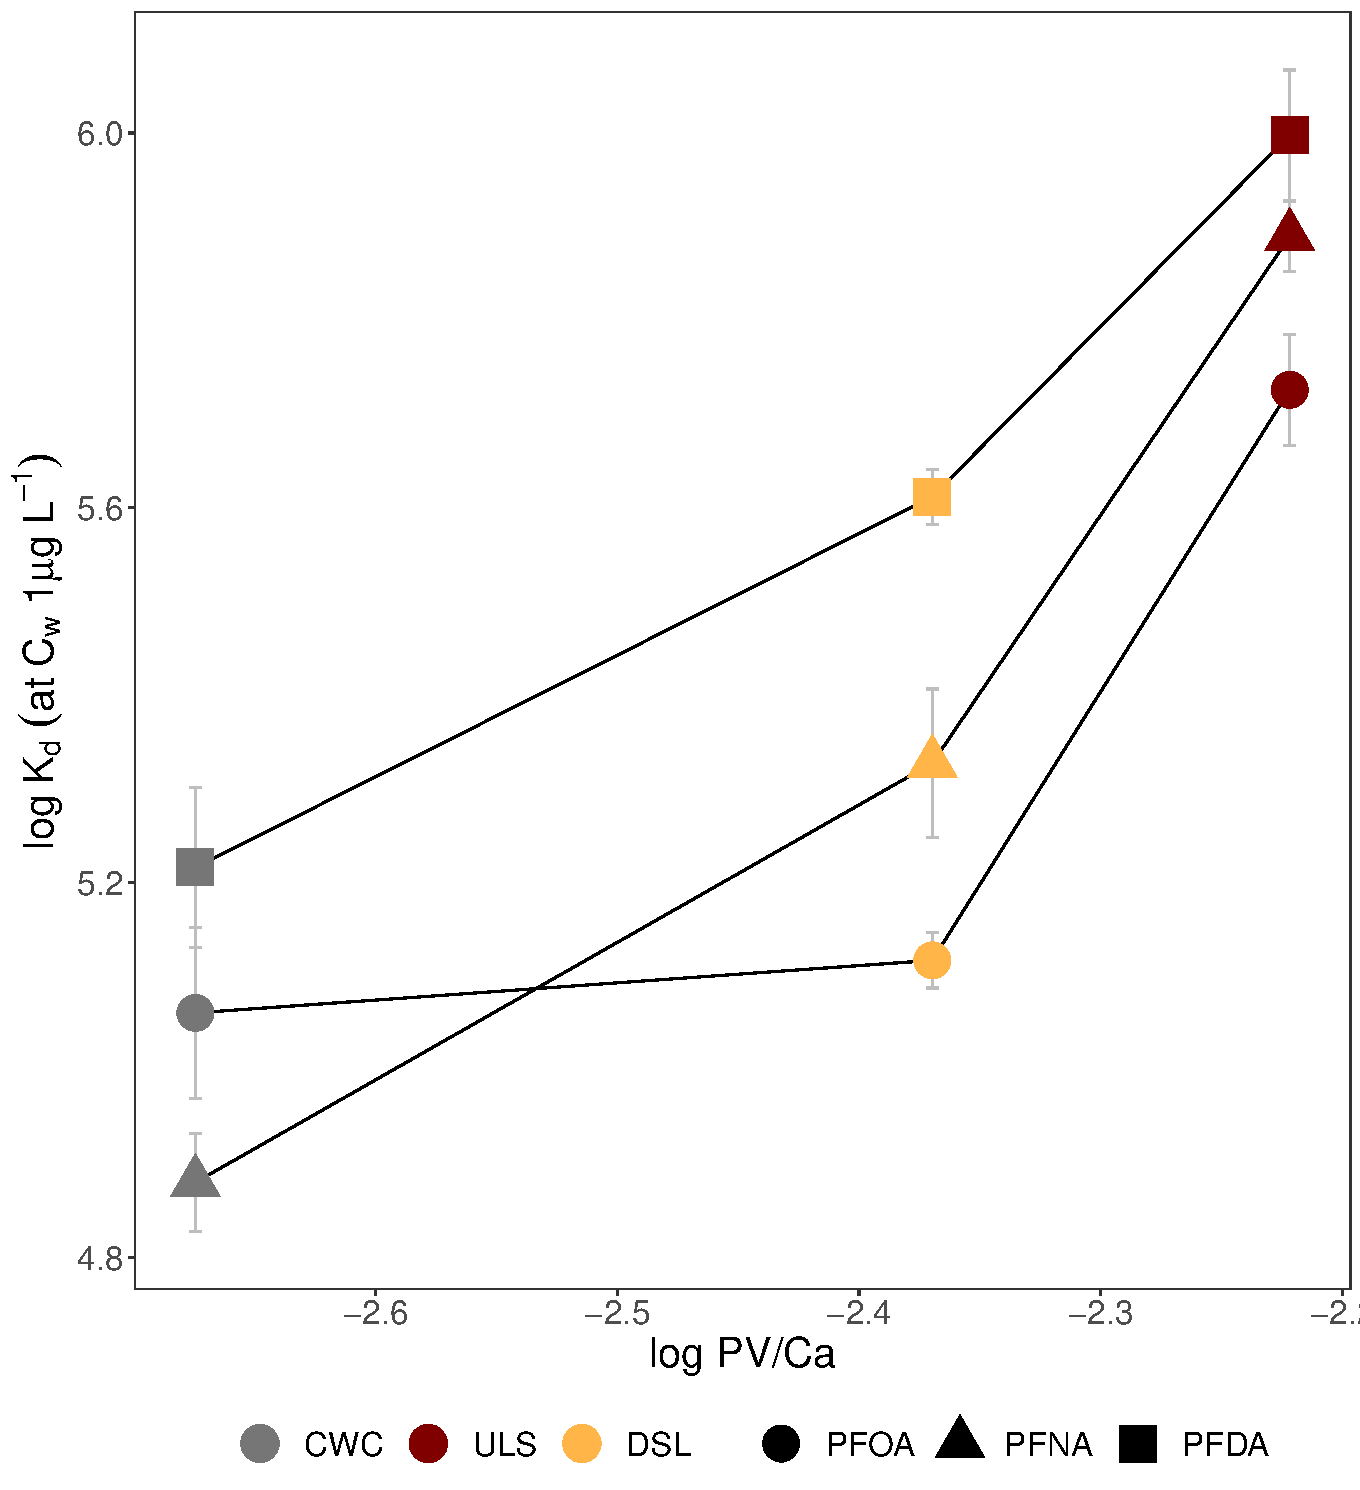
\includegraphics[height=5cm]{R/figs/Kd_1ugL_PVN2_Ca.pdf}
        \caption{}
        \label{subfig:PVN2_Ca}
    \end{subfigure}
\end{figure*}
\begin{figure*}[t]\ContinuedFloat
    \begin{subfigure}[t]{0.5\textwidth}
        \centering
        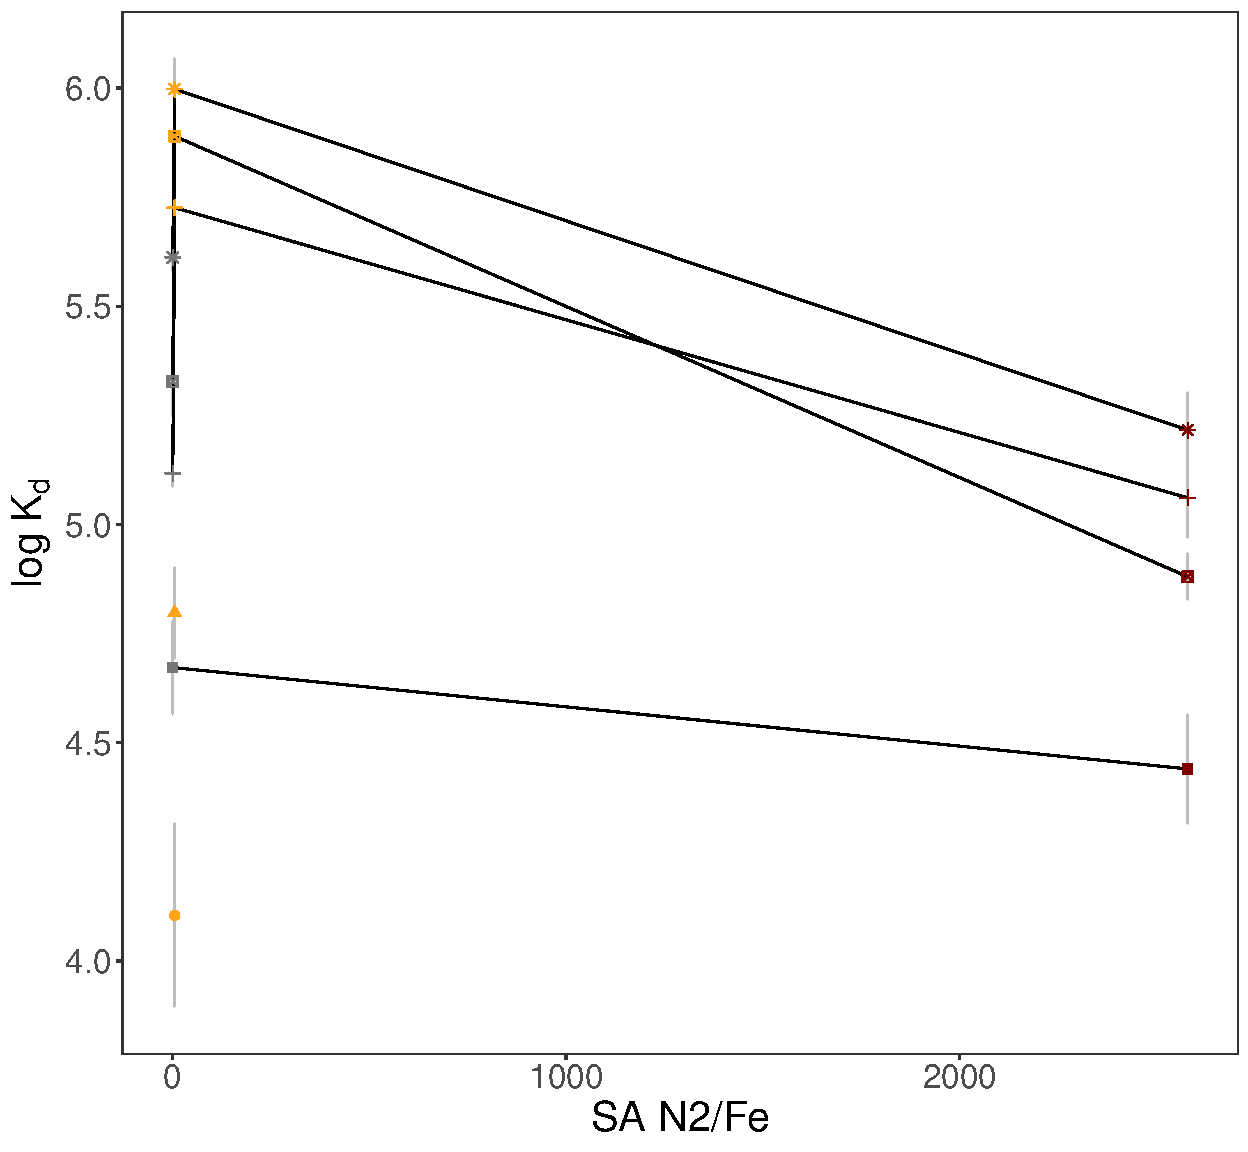
\includegraphics[height=5cm]{R/figs/Kd_1ugL_SAN2_Fe.pdf}
        \caption{}
        \label{subfig:SAN2_Fe}
    \end{subfigure}%
    ~ 
    \begin{subfigure}[t]{0.5\textwidth}
        \centering
        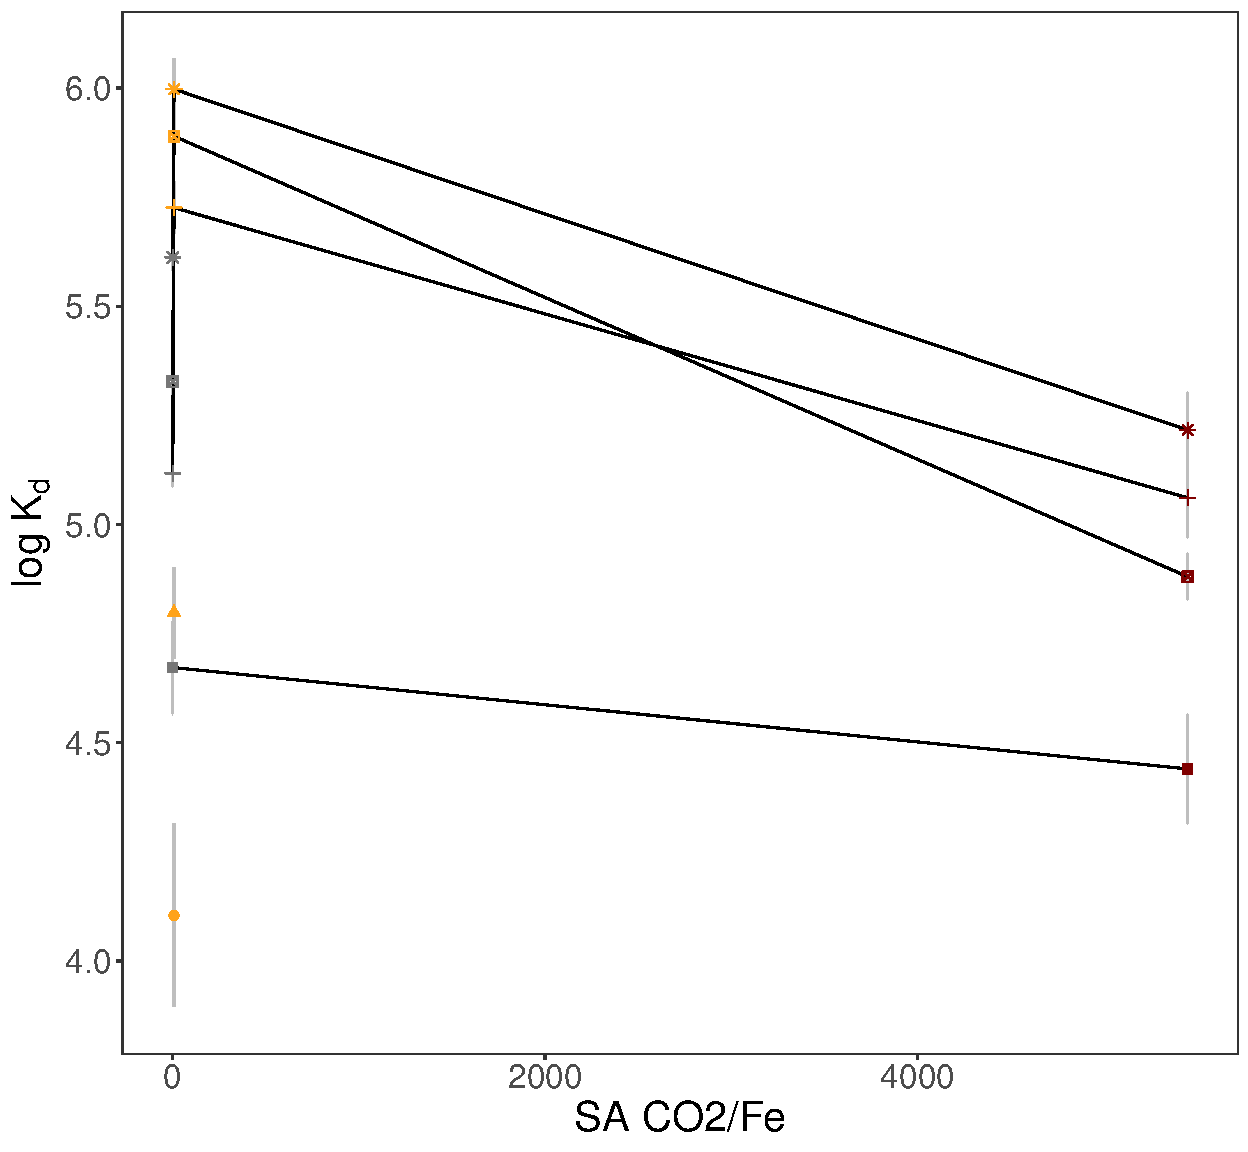
\includegraphics[height=5cm]{R/figs/Kd_1ugL_SACO2_Fe.pdf}
        \caption{}
        \label{subfig:SACO2_Fe}
    \end{subfigure}
    \medskip
    \begin{subfigure}[t]{0.5\textwidth}
        \centering
        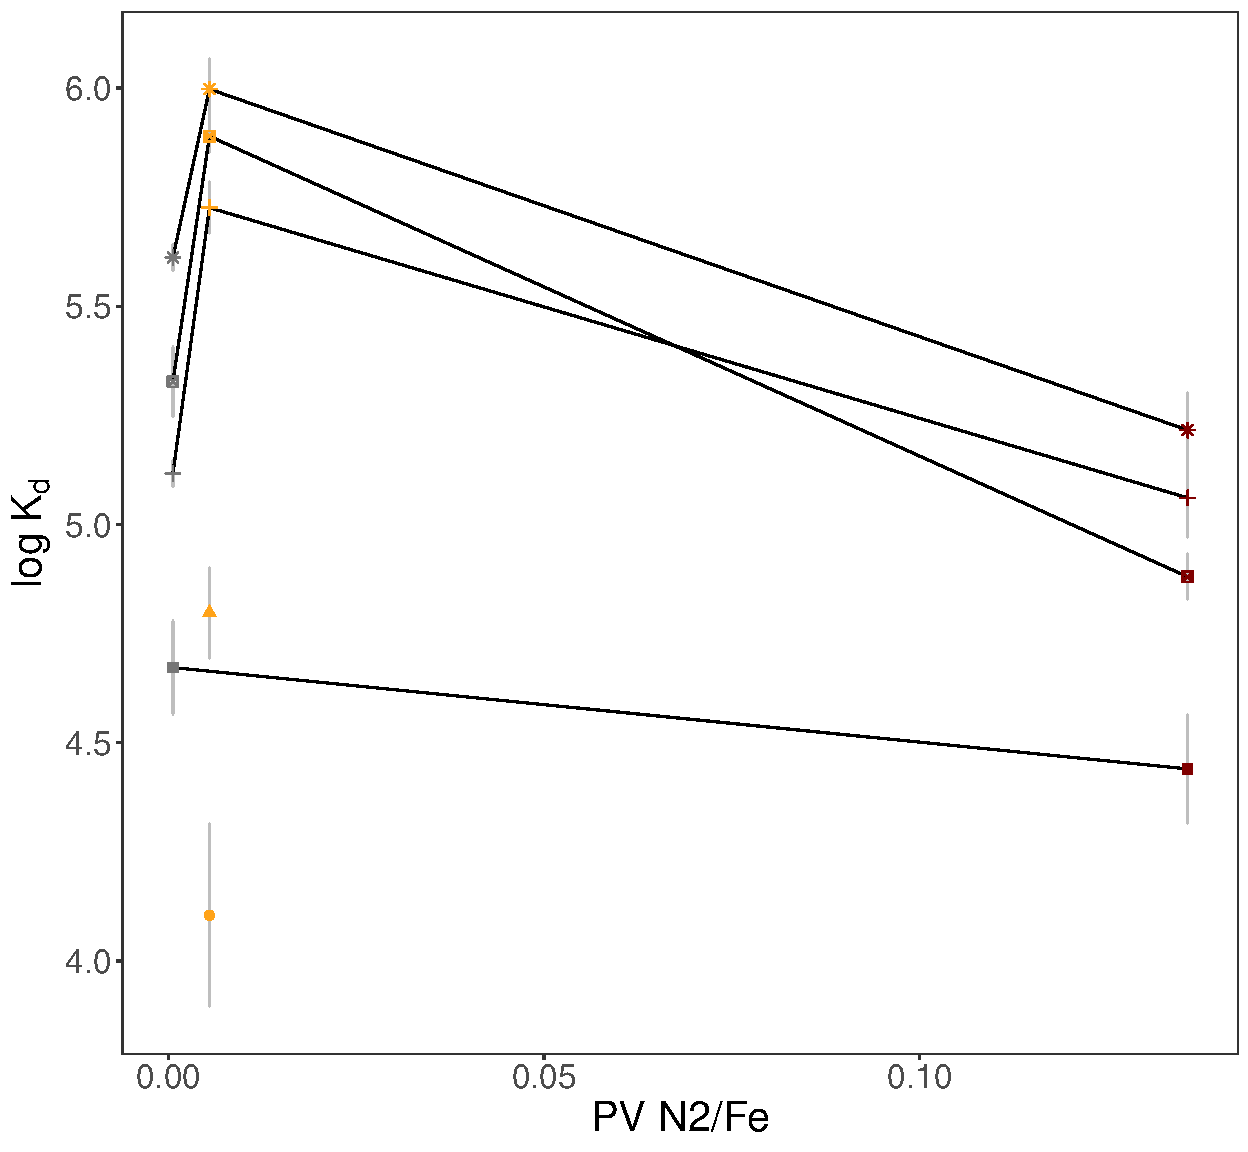
\includegraphics[height=5cm]{R/figs/Kd_1ugL_PVN2_Fe.pdf}
        \caption{}
        \label{subfig:PVN2_Fe}
    \end{subfigure}%
    ~ 
    \begin{subfigure}[t]{0.5\textwidth}
        \centering
        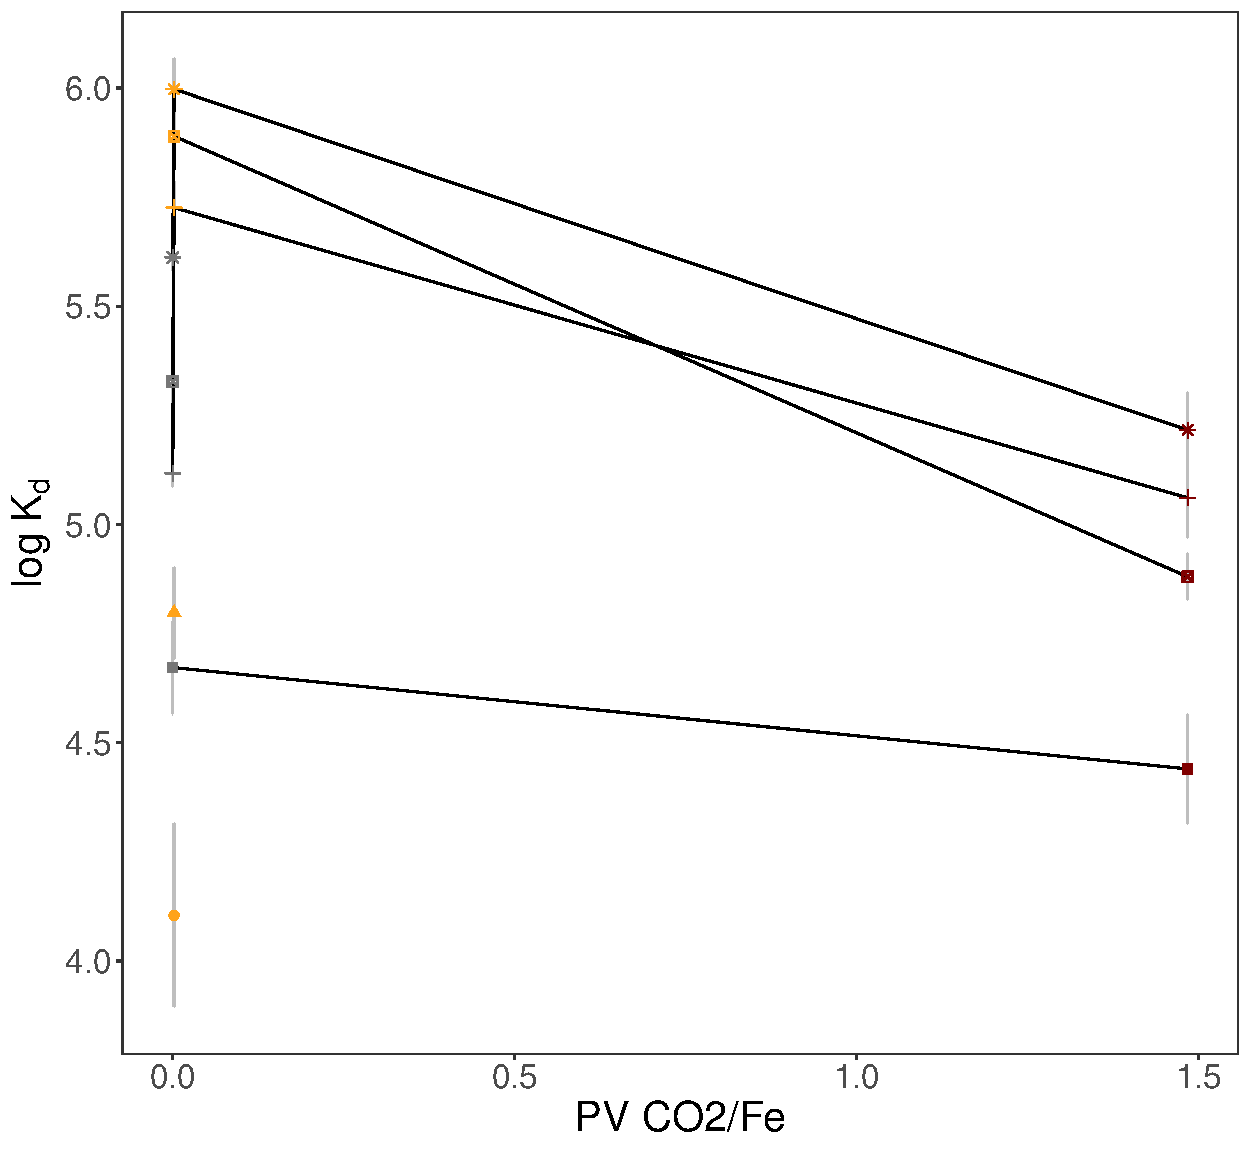
\includegraphics[height=5cm]{R/figs/Kd_1ugL_PVCO2_Fe.pdf}
        \caption{}
        \label{subfig:PVCO2_Fe}
    \end{subfigure}
    \label{fig:PVSA_Fe}
    \caption{}
\end{figure*}

\begin{figure}[!ht]
\subfloat[\label{subfig:SA_large}]{%
  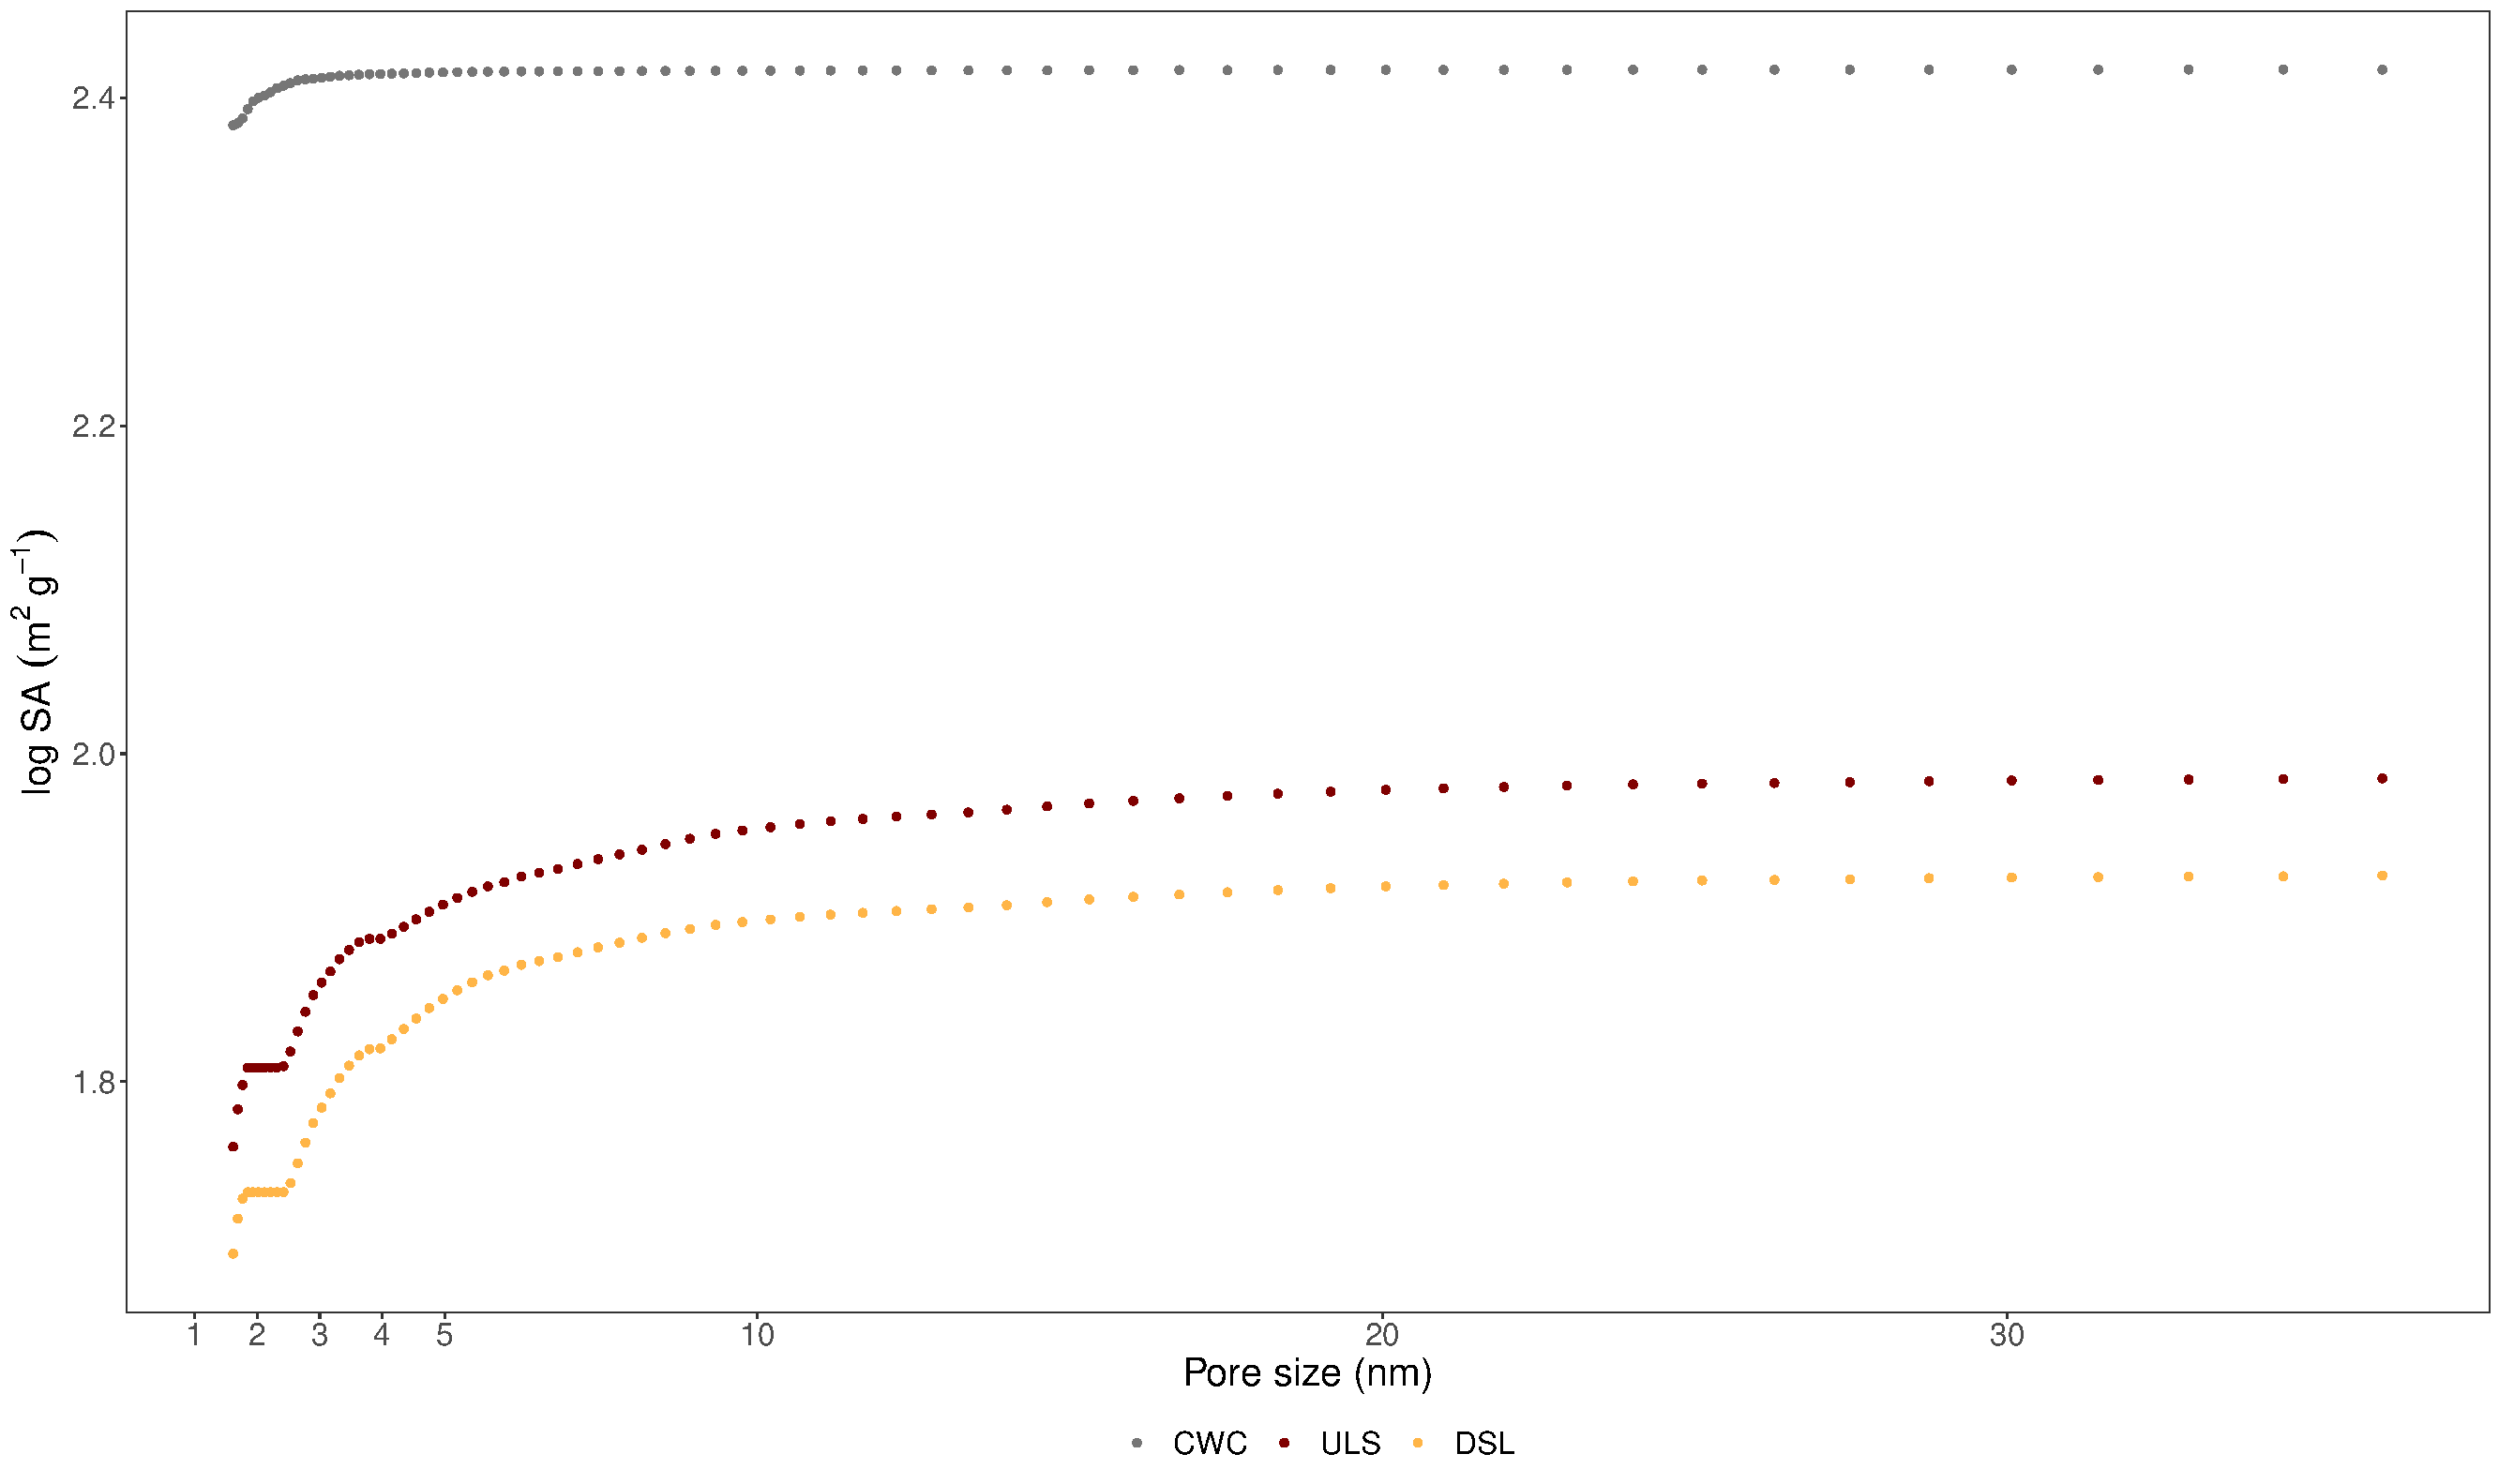
\includegraphics[width=0.5\textwidth]{R/figs/SA_large.pdf}
}
\hfill
\subfloat[\label{subfig:PV_large}]{%
  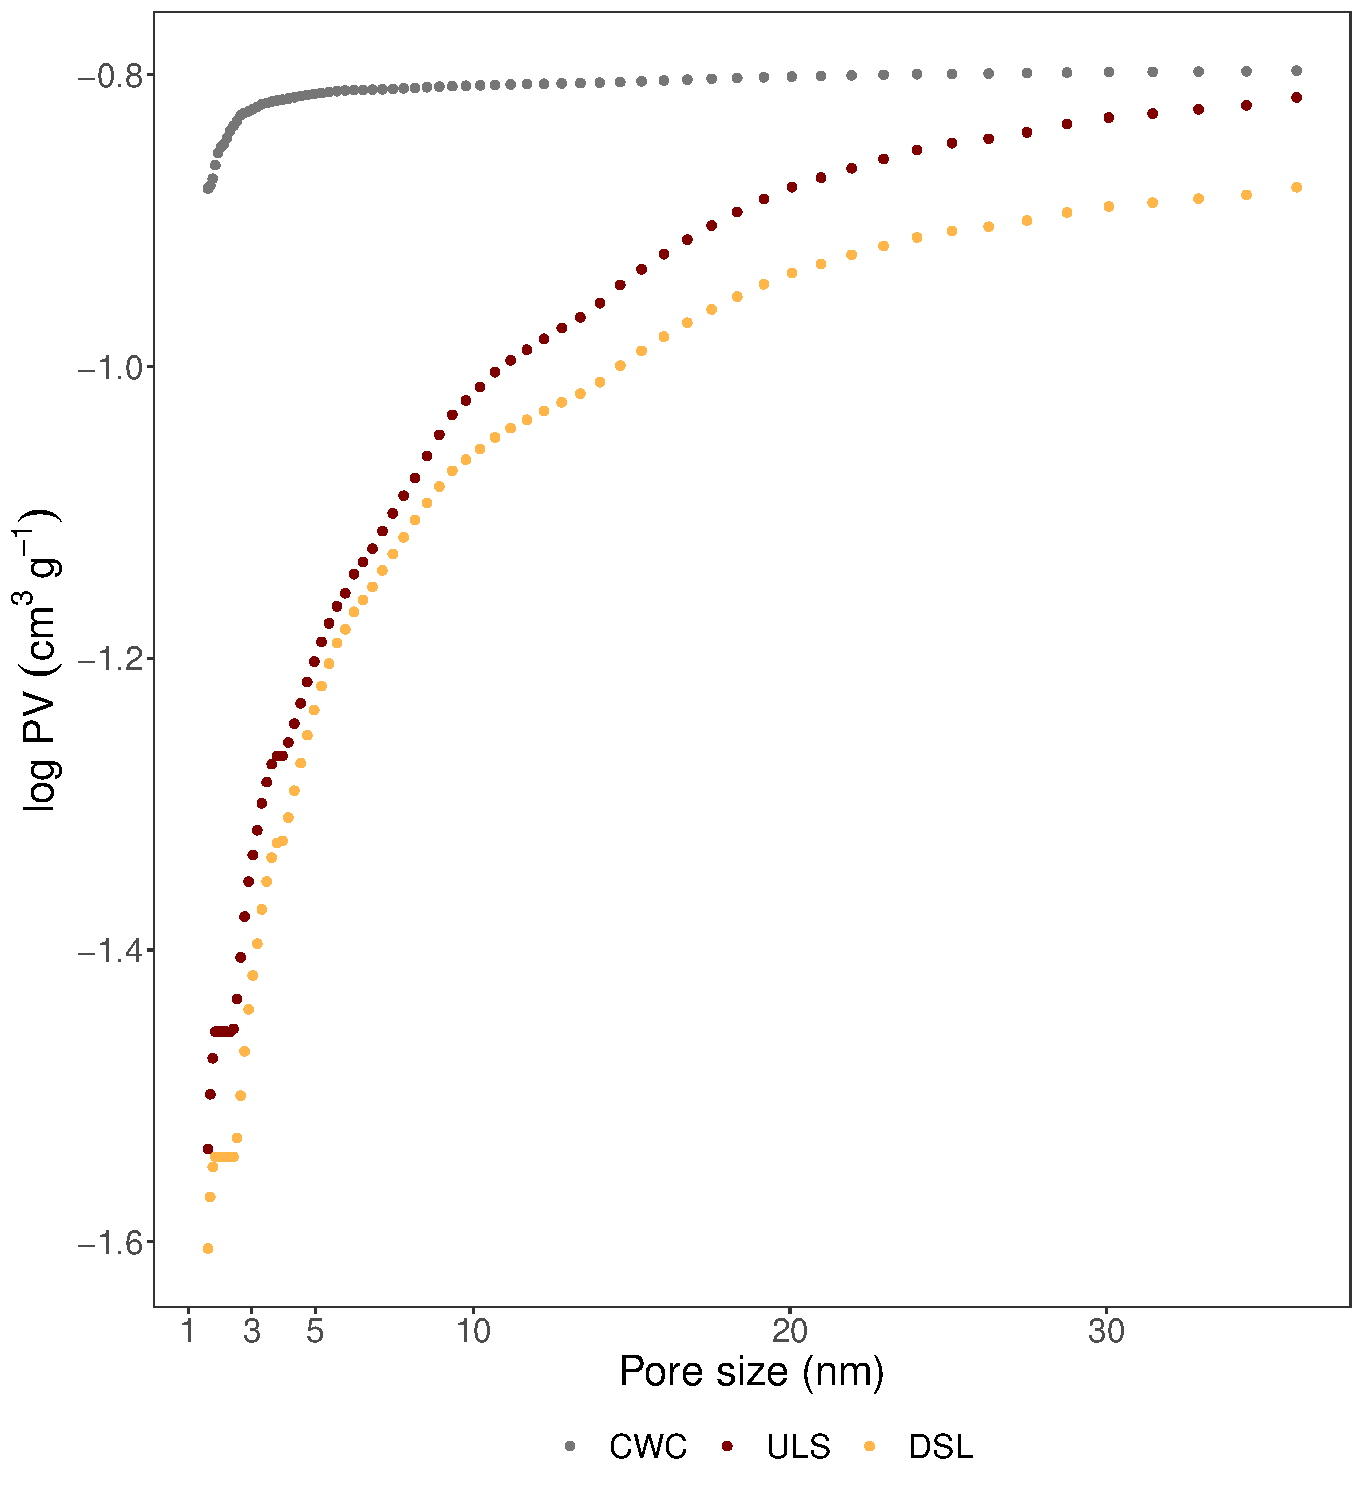
\includegraphics[width=0.5\textwidth]{R/figs/PV_large.pdf}
}
\medskip
\subfloat[\label{subfig:SAPV_large}]{%
  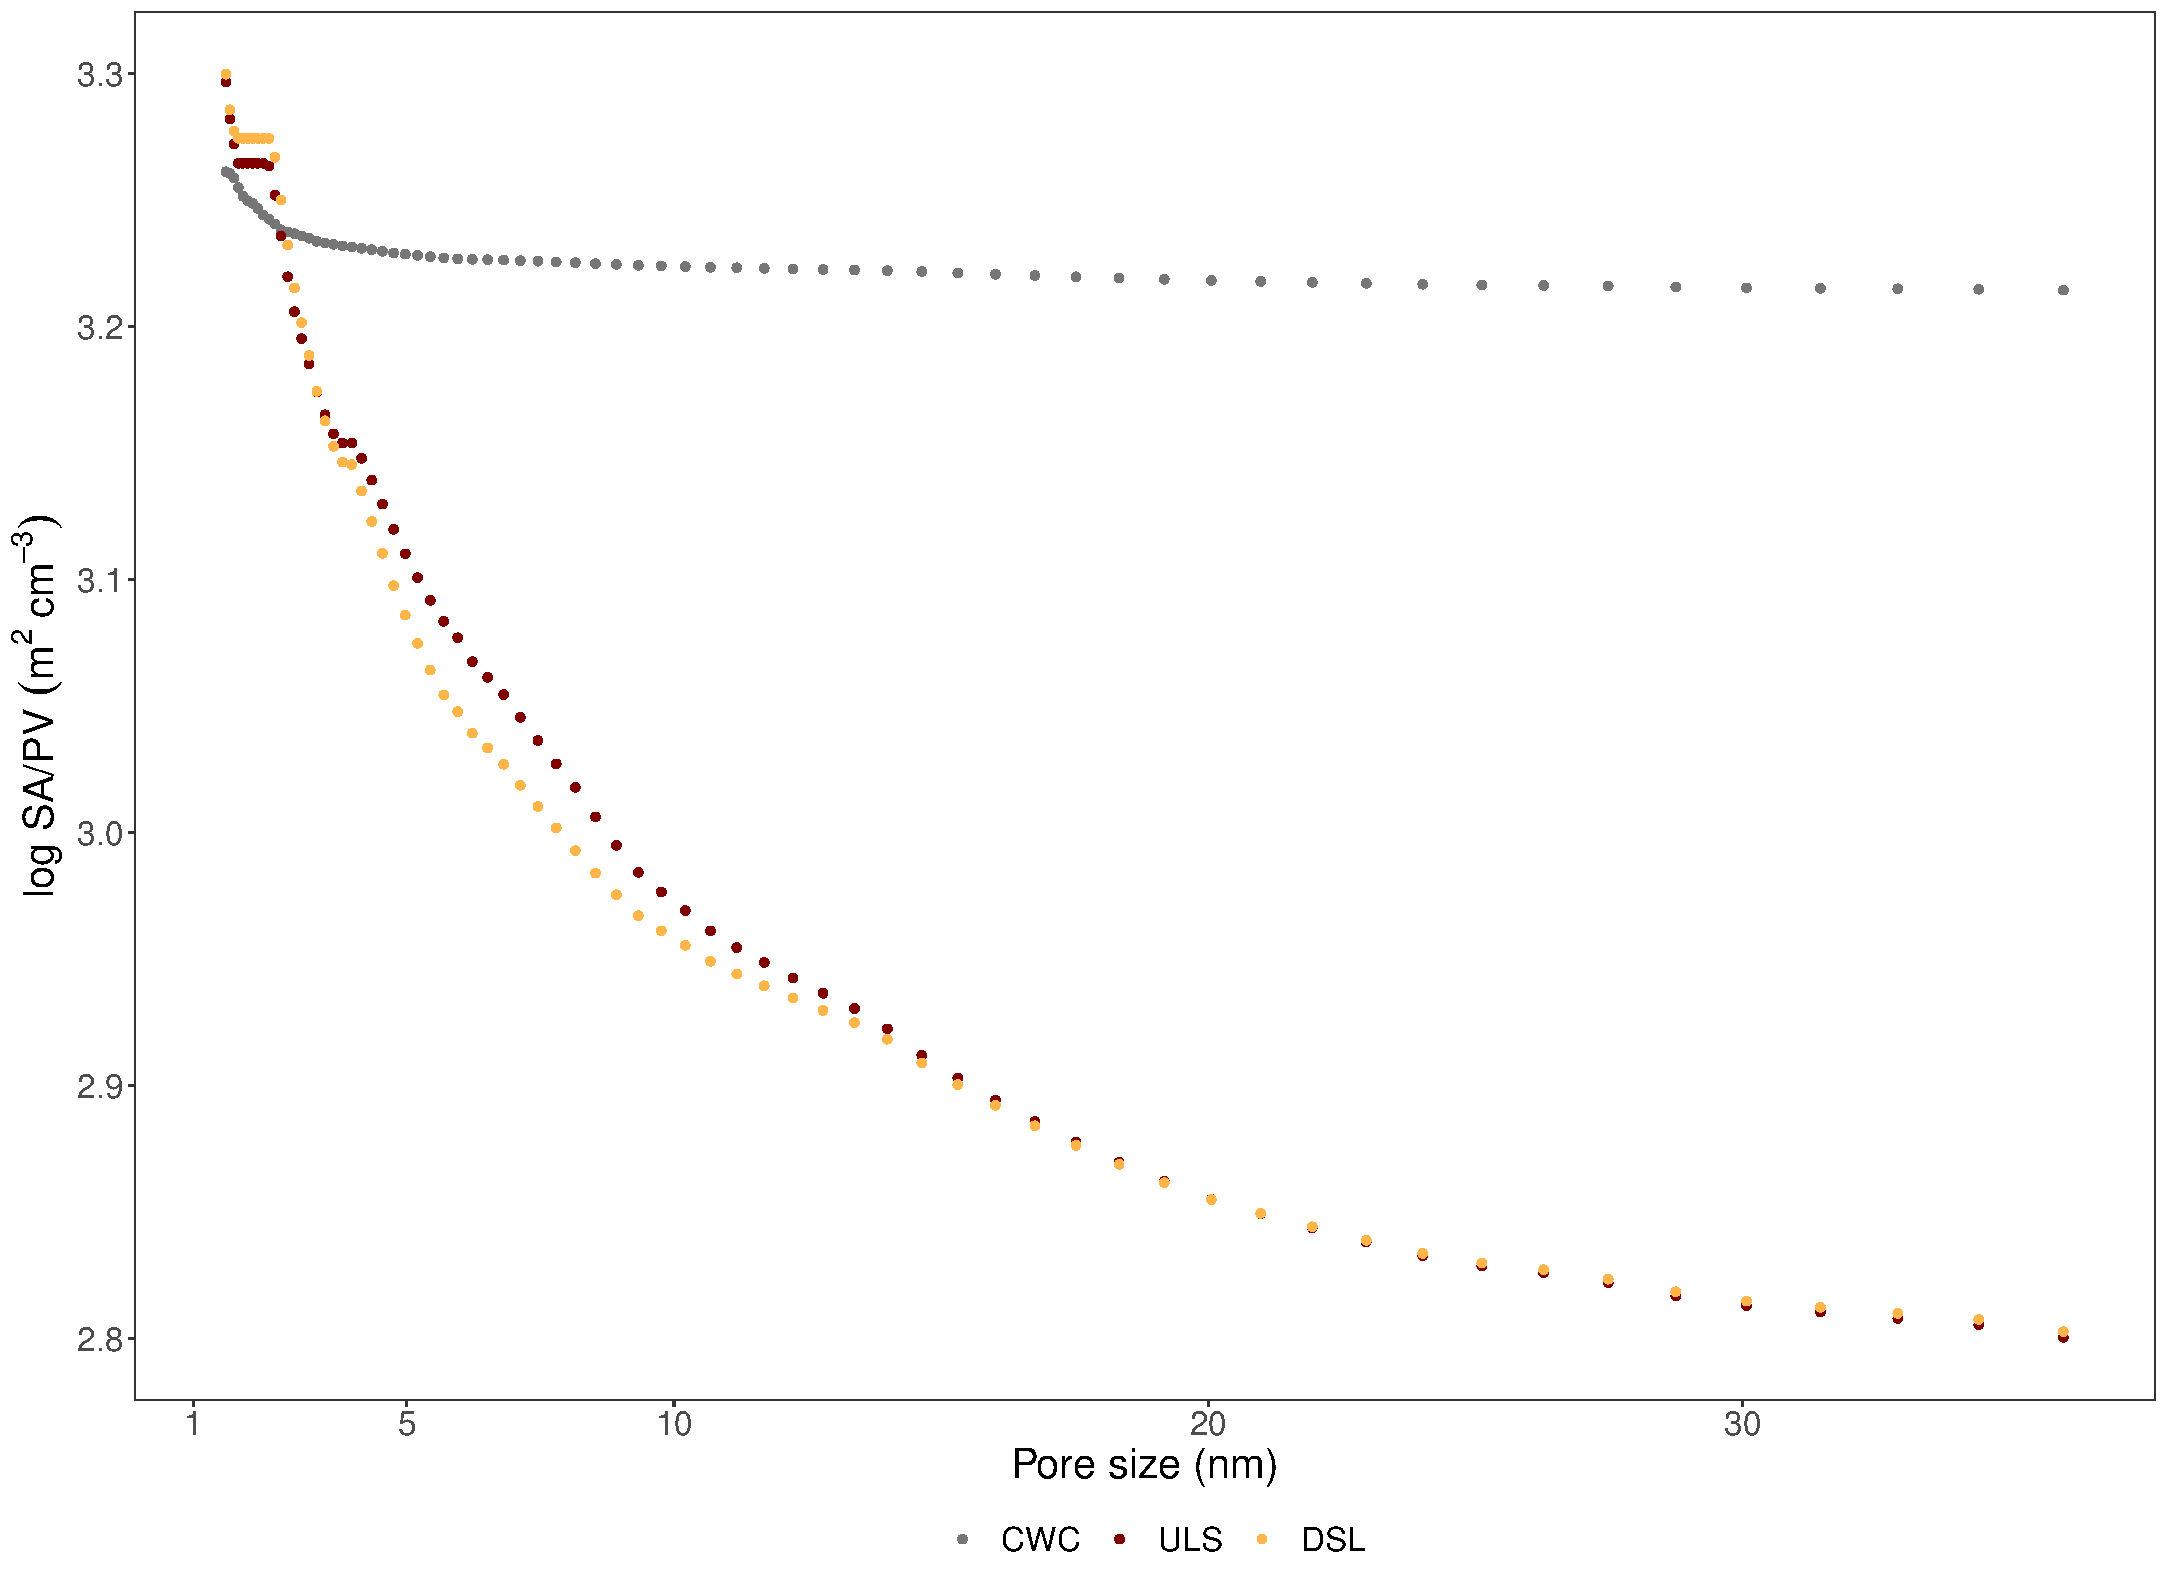
\includegraphics[width=0.5\textwidth]{R/figs/SAPV_large.pdf}
}
\hfill
\subfloat[\label{subfig:SAPV_C_large}]{%
  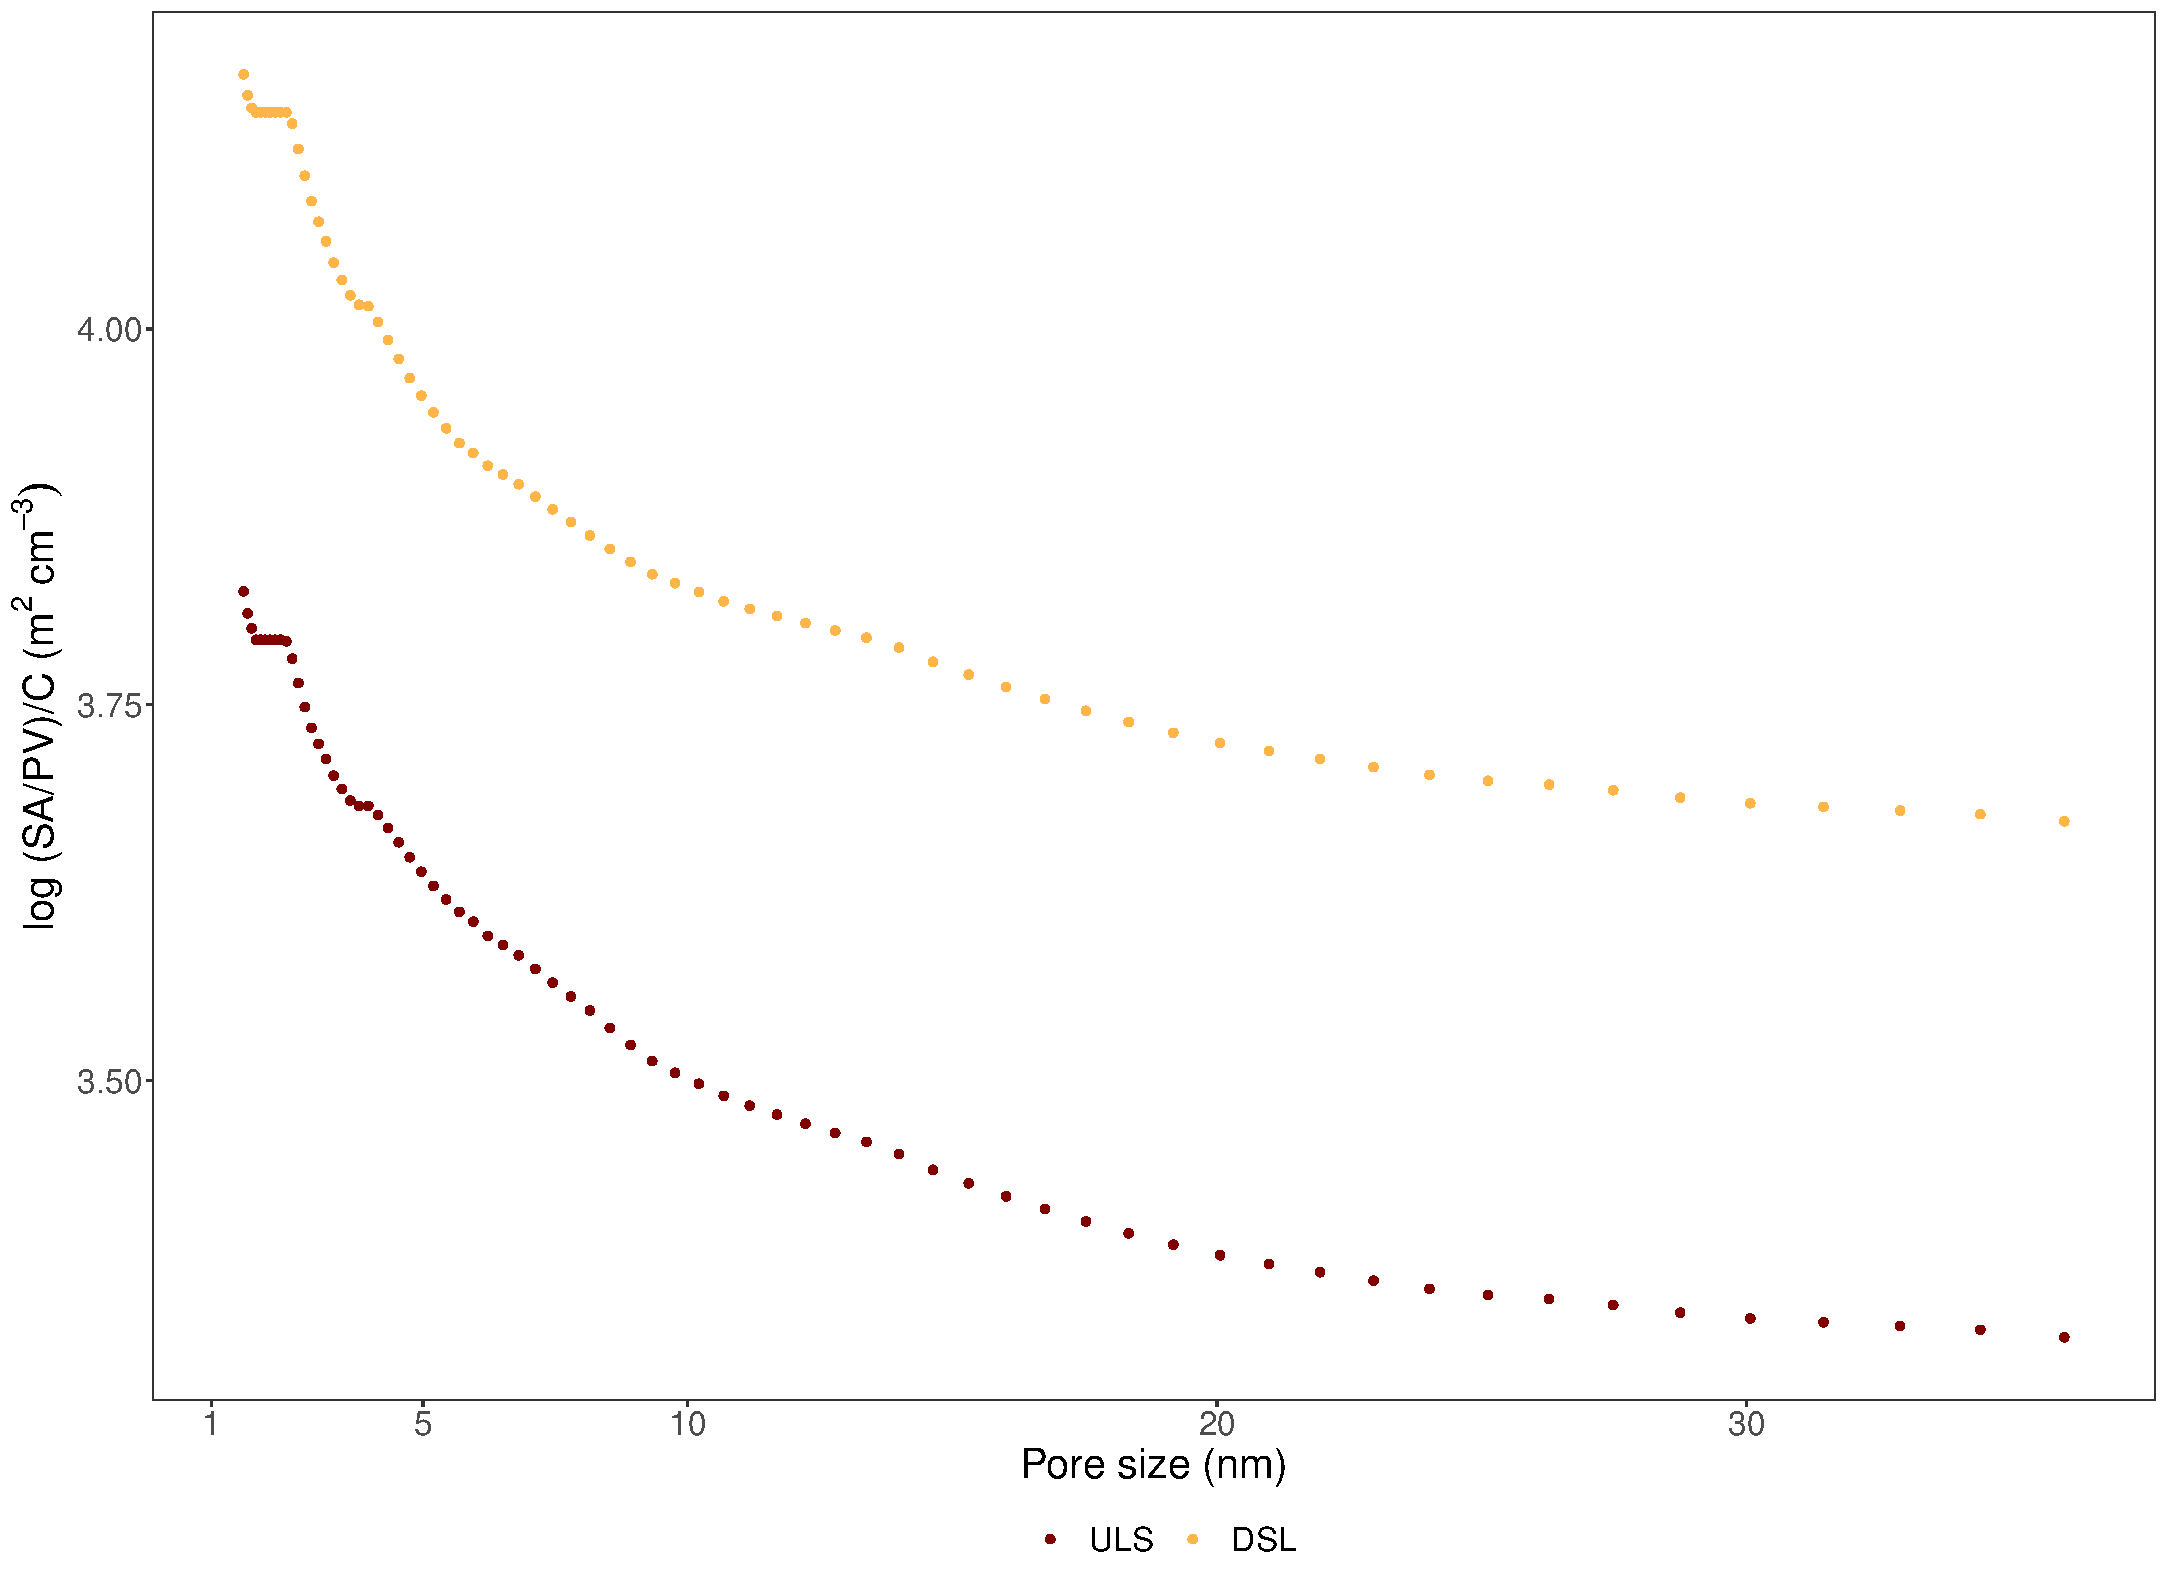
\includegraphics[width=0.5\textwidth]{R/figs/SAPV_C_large.pdf}
}
\caption{Pore size distribution for pores $>$ 1.5 nm. (a) Surface area, (b) pore volume, (c) SA/PV ratio for pores $>$1.5 nm normalized to carbon content (g C g BC\textsuperscript{-1}). (d) A lower SA/PV/C ratio indicates a higher degree of C in the pore wall matrix.}
\label{fig:PZD}
\end{figure}

\begin{figure*}[ht]
\centering
    \begin{subfigure}[t]{0.5\textwidth}
        \centering
        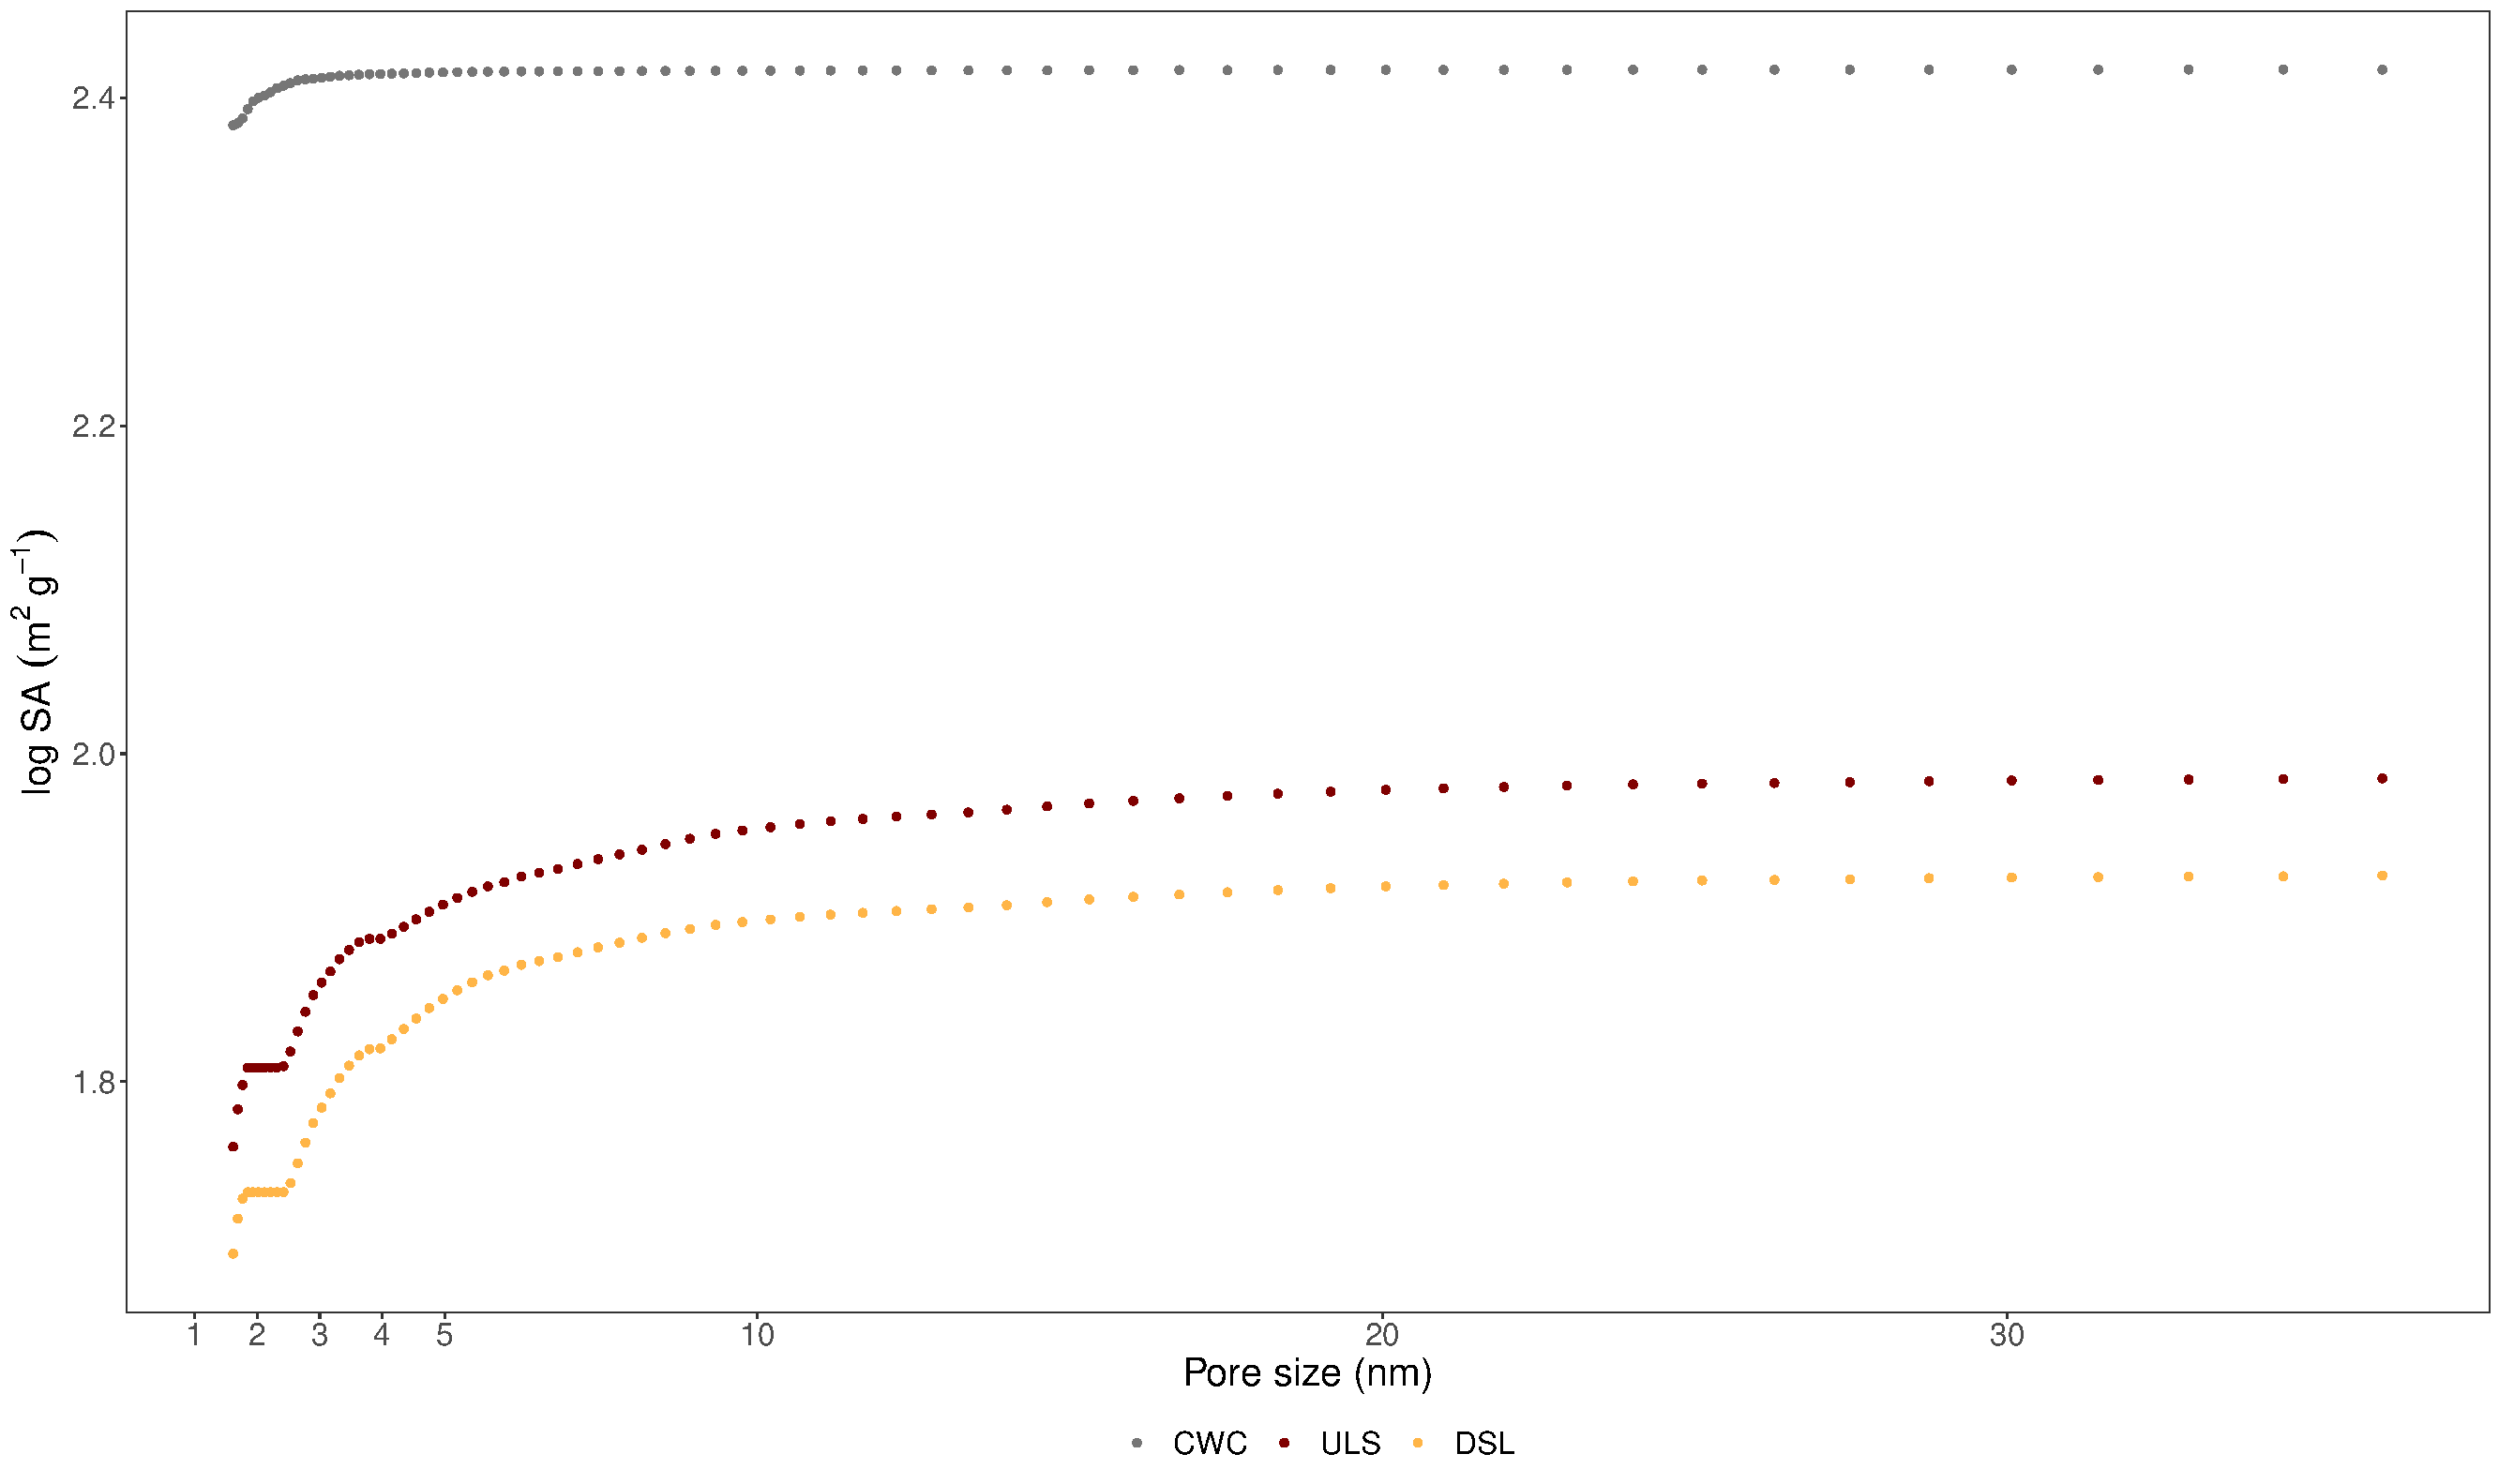
\includegraphics[\textwidth]{R/figs/SA_large.pdf}
        \caption{}
        \label{subfig:SA_large}
    \end{subfigure}%
    ~ 
    \begin{subfigure}[t]{0.5\textwidth}
        \centering
        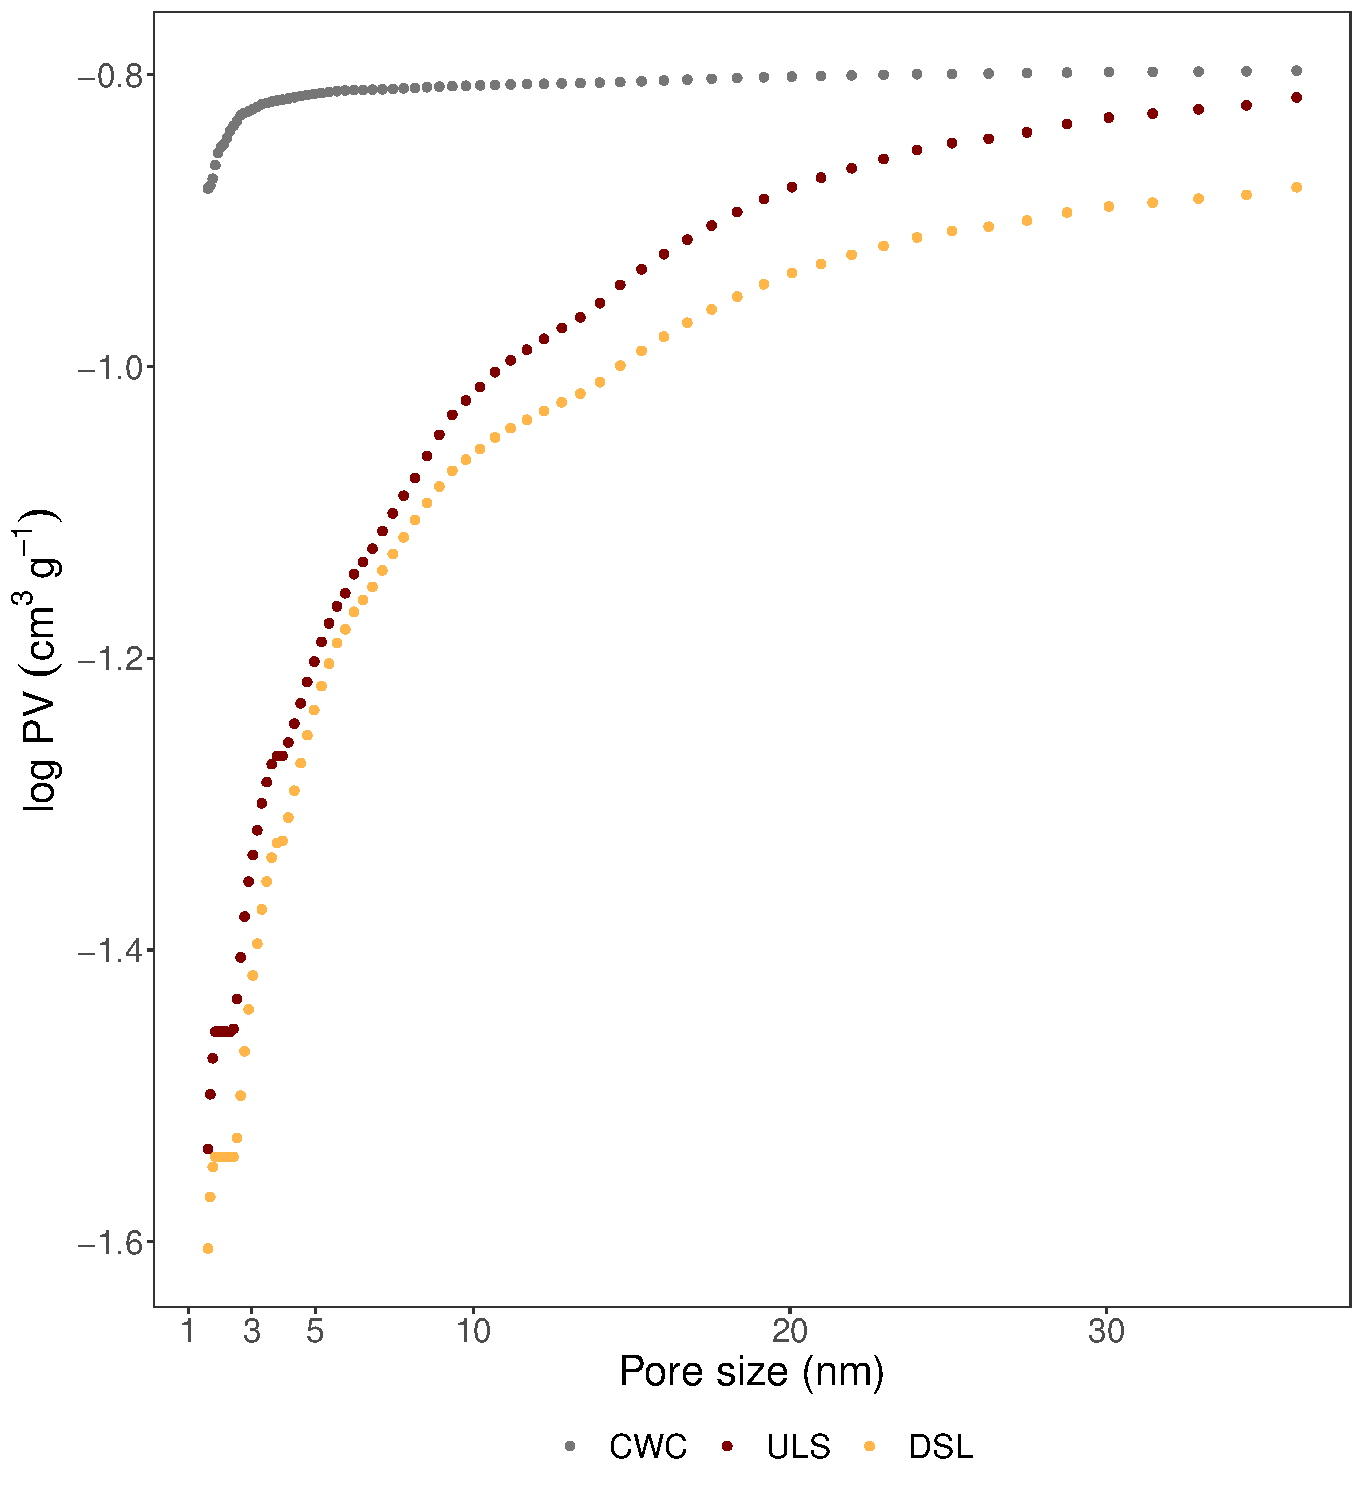
\includegraphics[\textwidth]{R/figs/PV_large.pdf}
        \caption{}
        \label{subfig:PV_large}
    \end{subfigure}
    \medskip
    \begin{subfigure}[t]{0.5\textwidth}
        \centering
        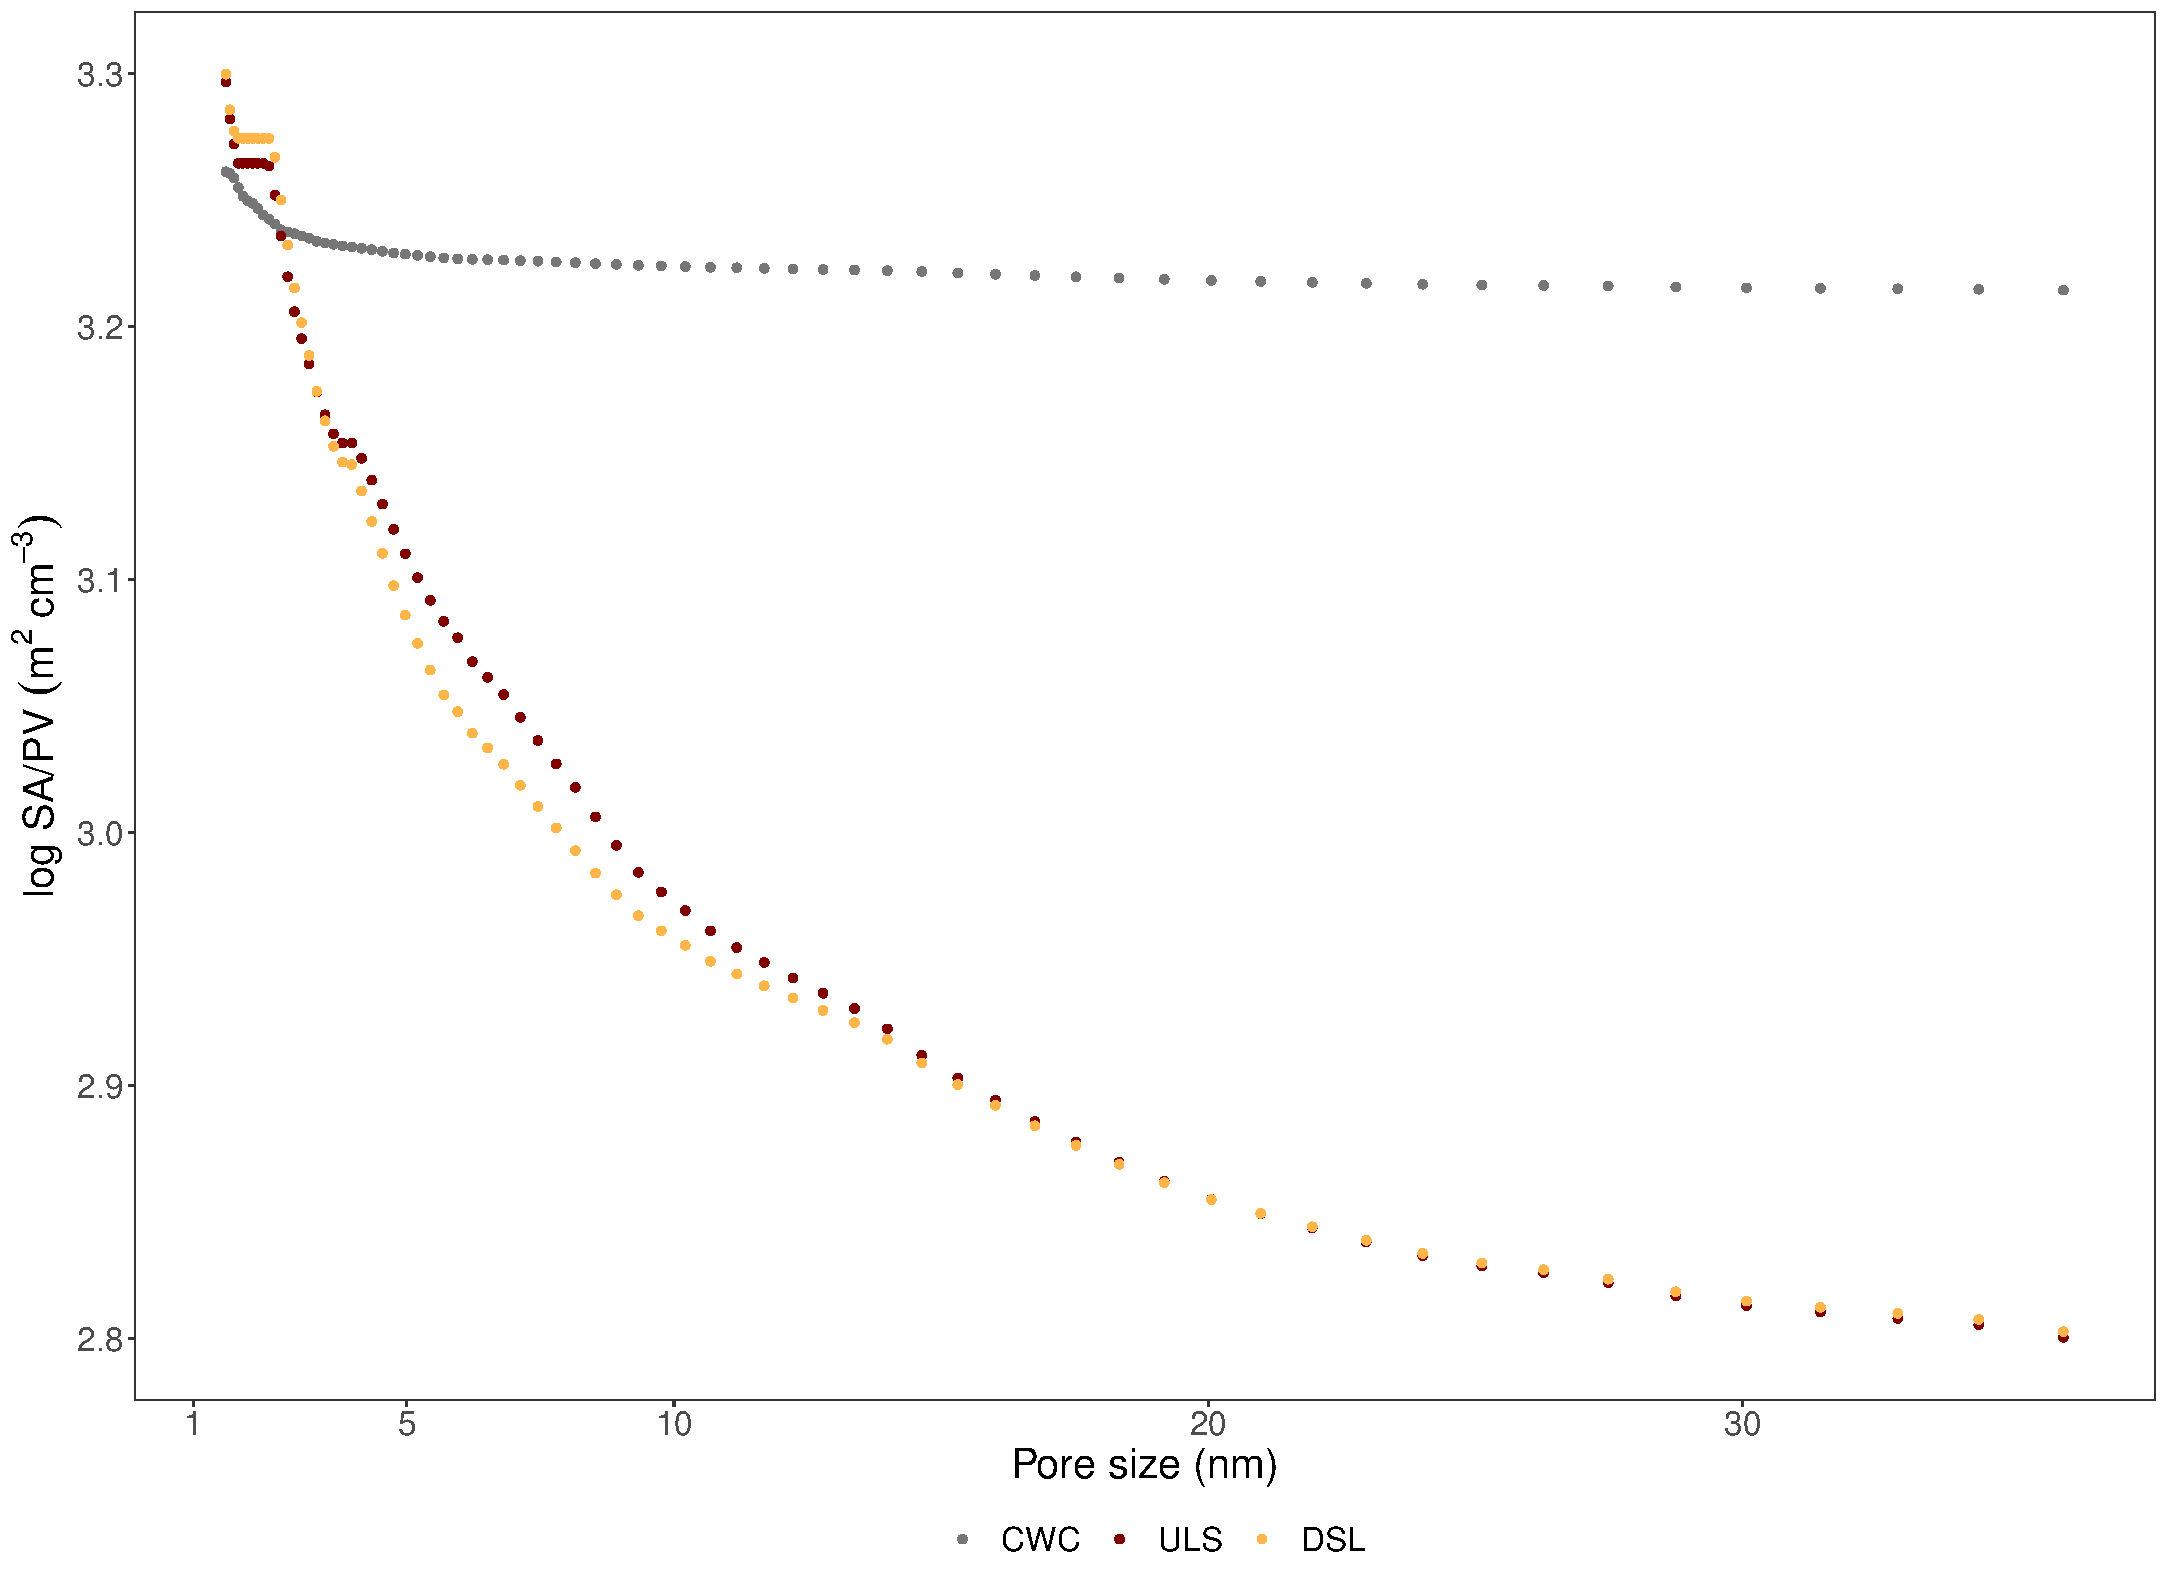
\includegraphics[\textwidth]{R/figs/SAPV_large.pdf}
        \caption{}
        \label{subfig:SAPV_large}
    \end{subfigure}%
    ~ 
    \begin{subfigure}[t]{0.5\textwidth}
        \centering
        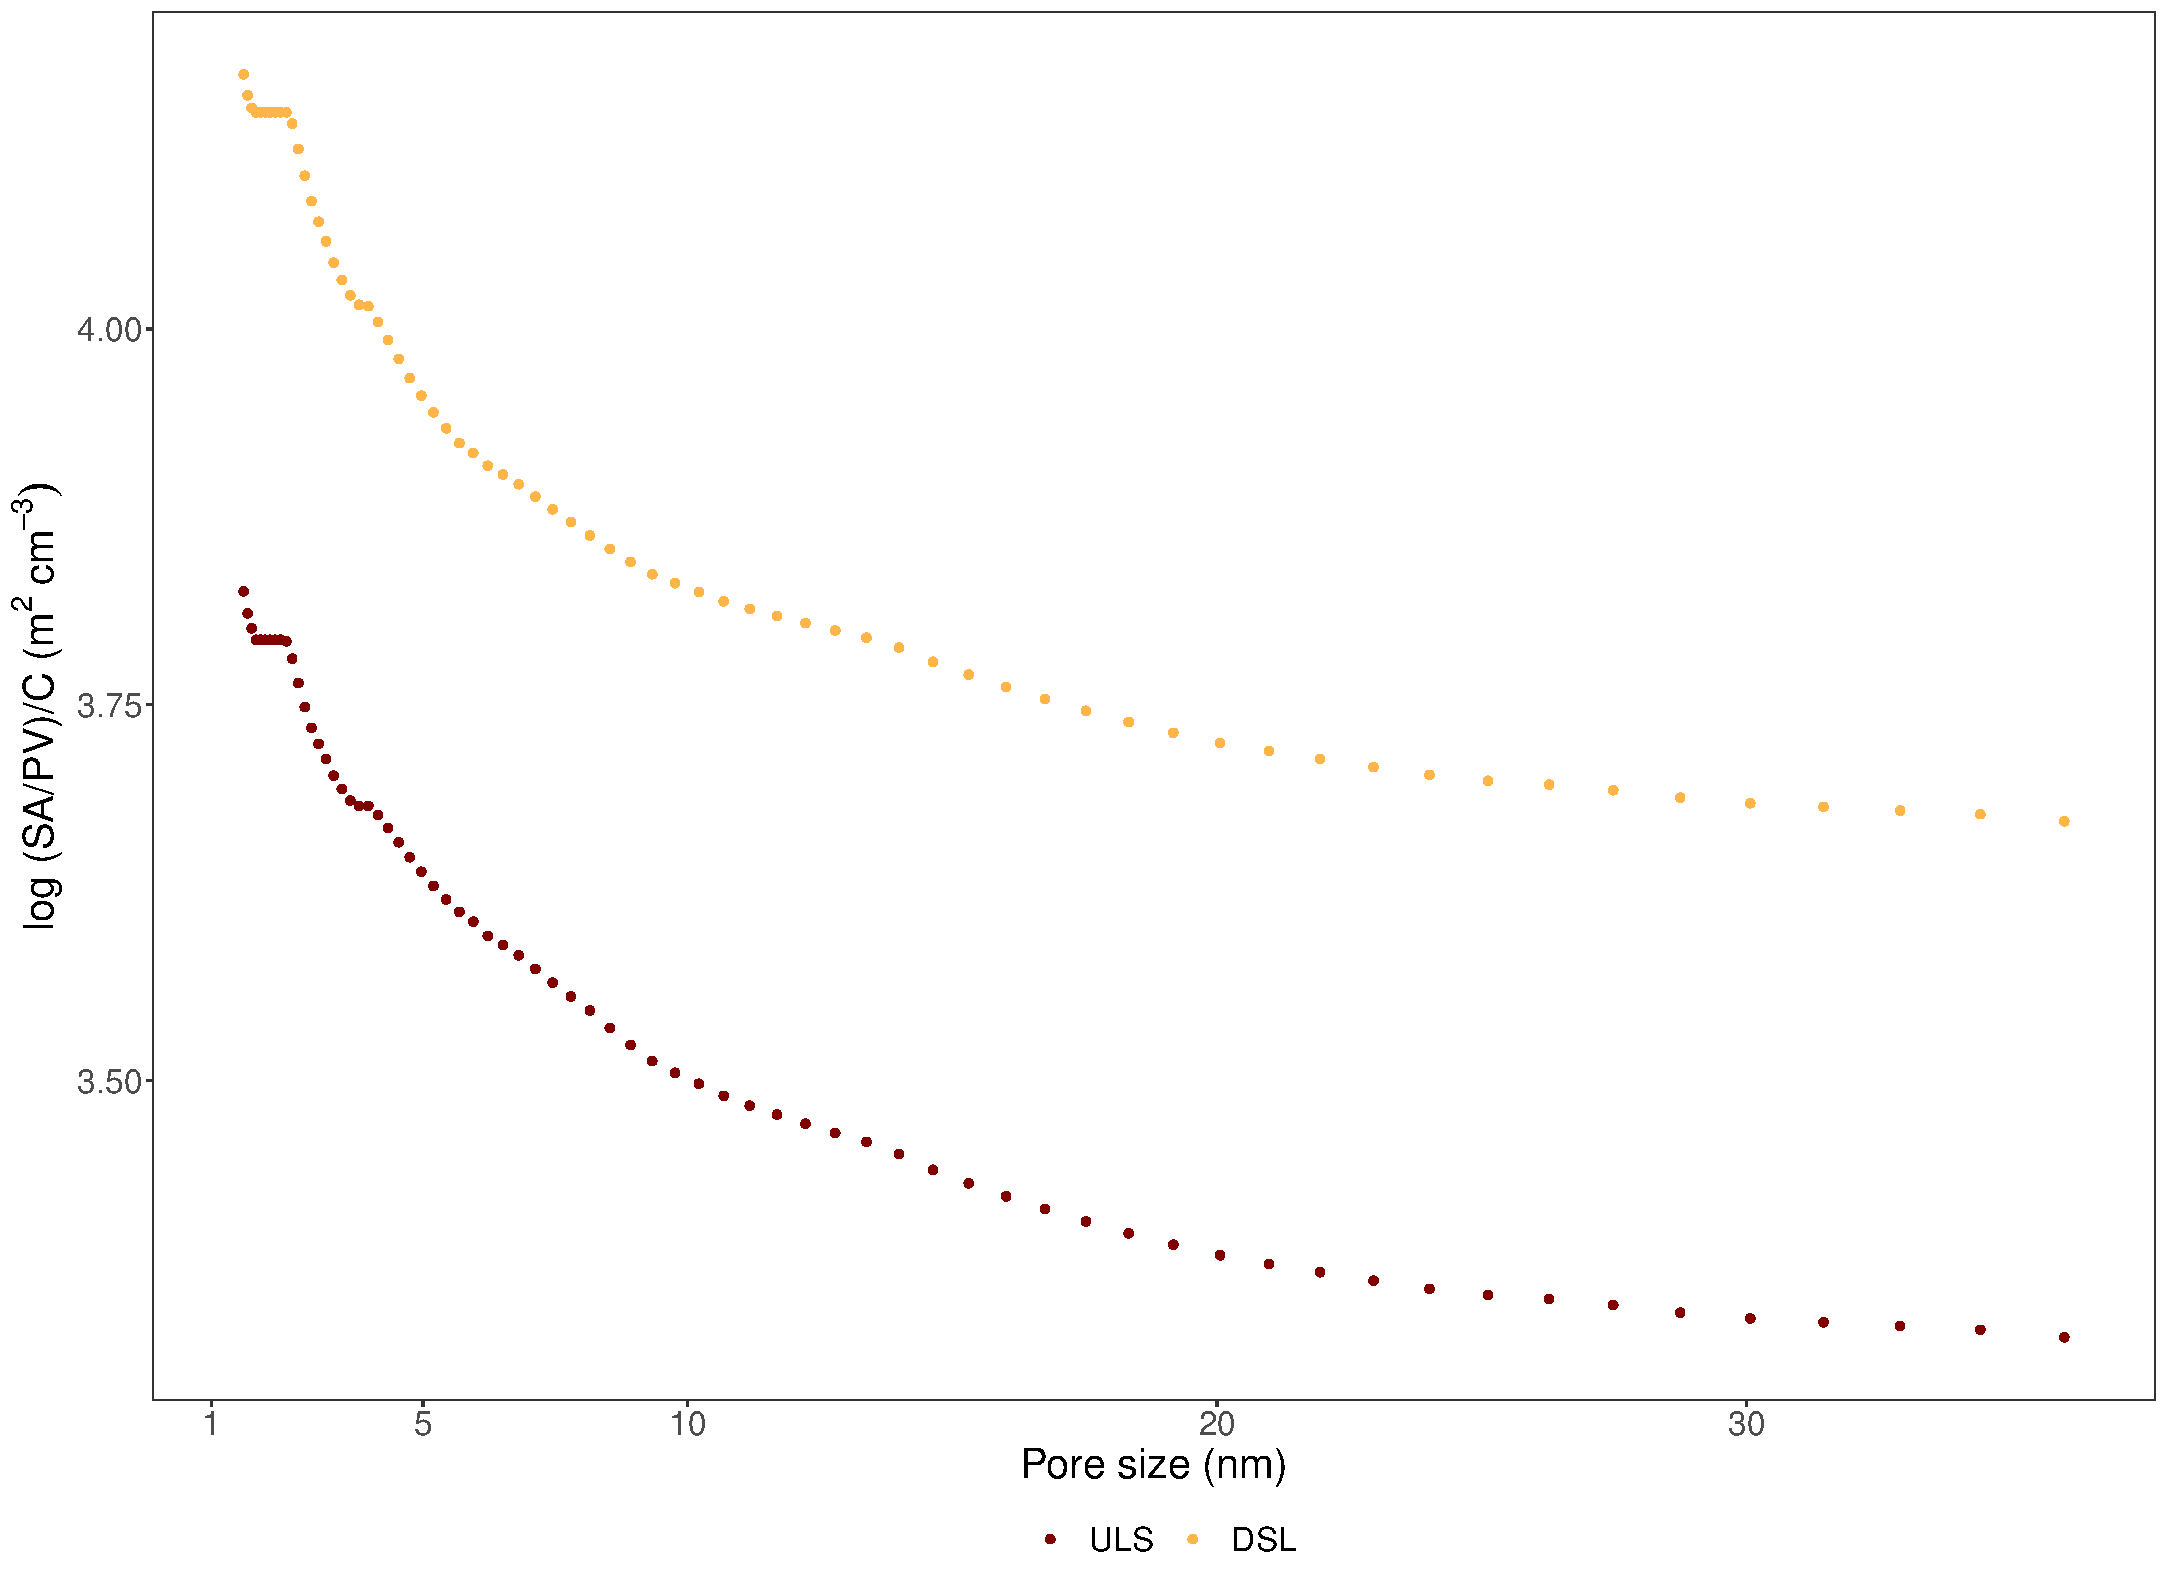
\includegraphics[\textwidth]{R/figs/SAPV_C_large.pdf}
        \caption{}
        \label{subfig:SAPV_C_large}
    \end{subfigure}
\caption{Pore size distribution for pores $>$ 1.5 nm. (a) Surface area, (b) pore volume, (c) SA/PV ratio for pores $>$1.5 nm normalized to carbon content (g C g BC\textsuperscript{-1}). (d) A lower SA/PV/C ratio indicates a higher degree of C in the pore wall matrix.}
\label{fig:PZD_large}
\end{figure*}

Pore size distribution is important for explaining sorption of PFAS of increasing chain lengths due to differences in molecular size. PFDA has a maximum diameter of 1.54 nm, and therefore experiences size exclusion for the smallest pores (0.5-1.5 nm) and can therefore only diffuse into the larger pores represented by N\textsubscript{2} (\textgreater 1.5 nm) (\cref{tab:molecsize}). Regardless of the critical separation at pore size greater/less than 1.5 nm, shorter-chain PFCAs is expected to diffuse more easily into the pores than the larger compounds.  

\begin{figure}[!ht]
\subfloat[\label{subfig:Kd_C}]{%
  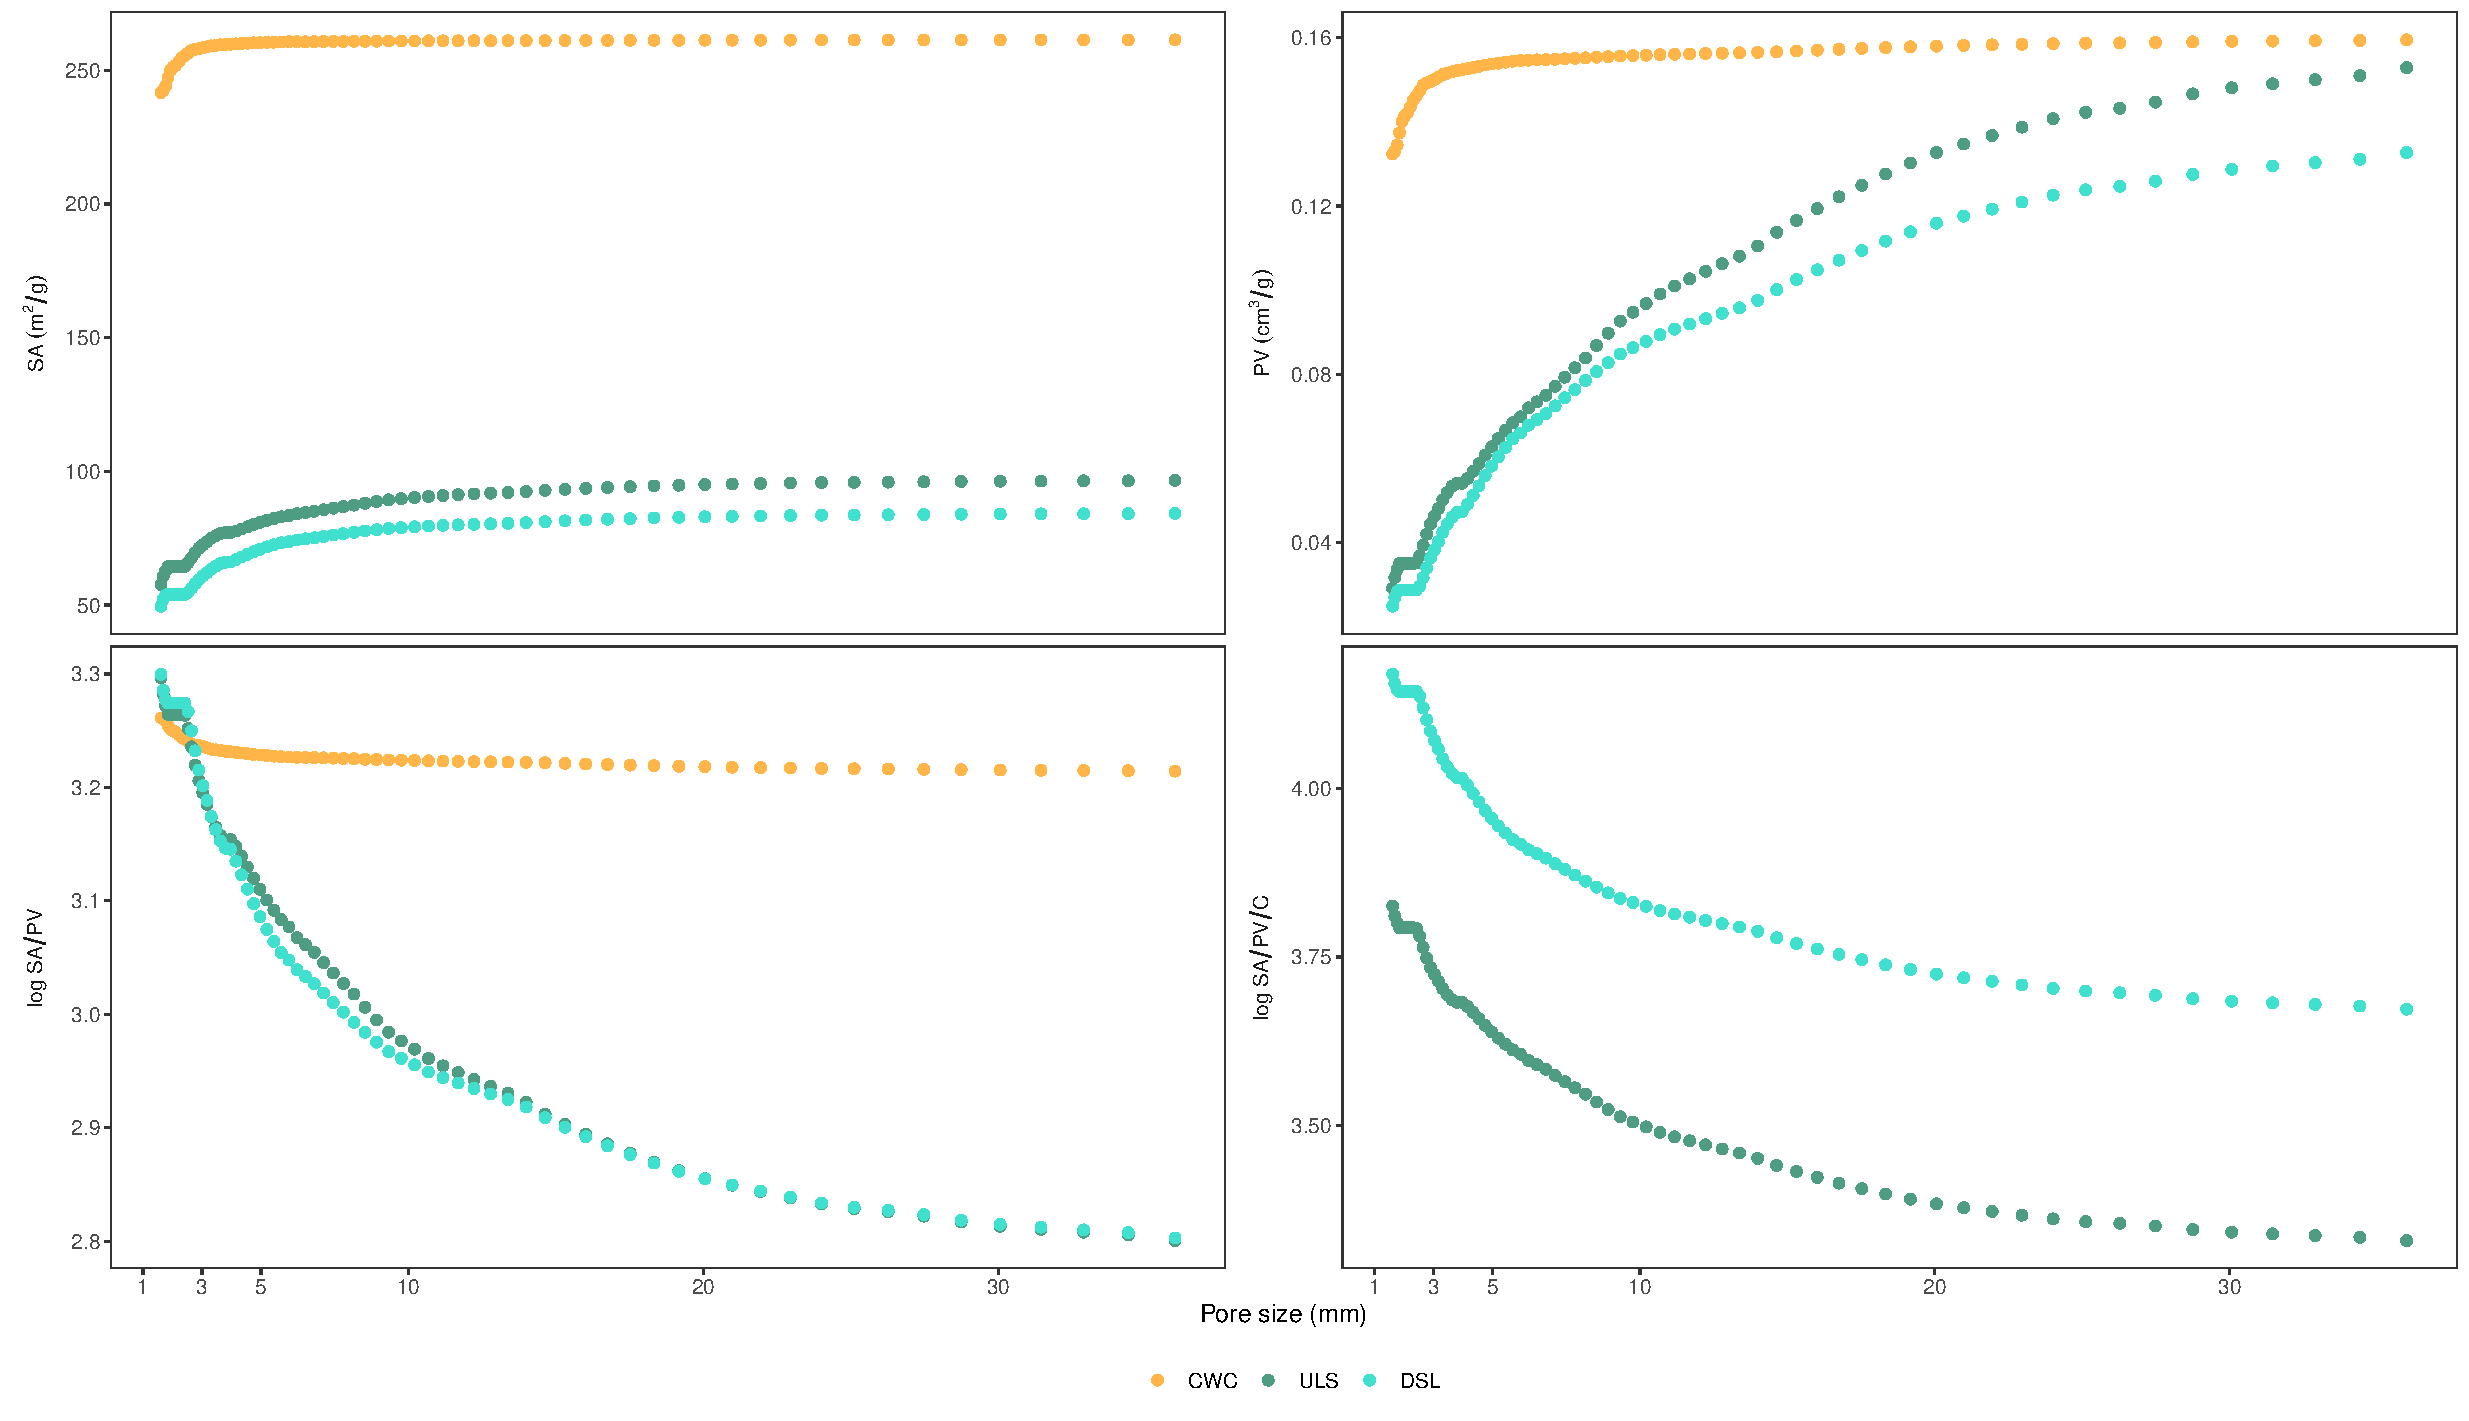
\includegraphics[width=0.3\textwidth]{R/figs/Kd_1ugL_C.pdf}
}
\hfill
\subfloat[\label{subfig:Kd_SAPV}]{%
  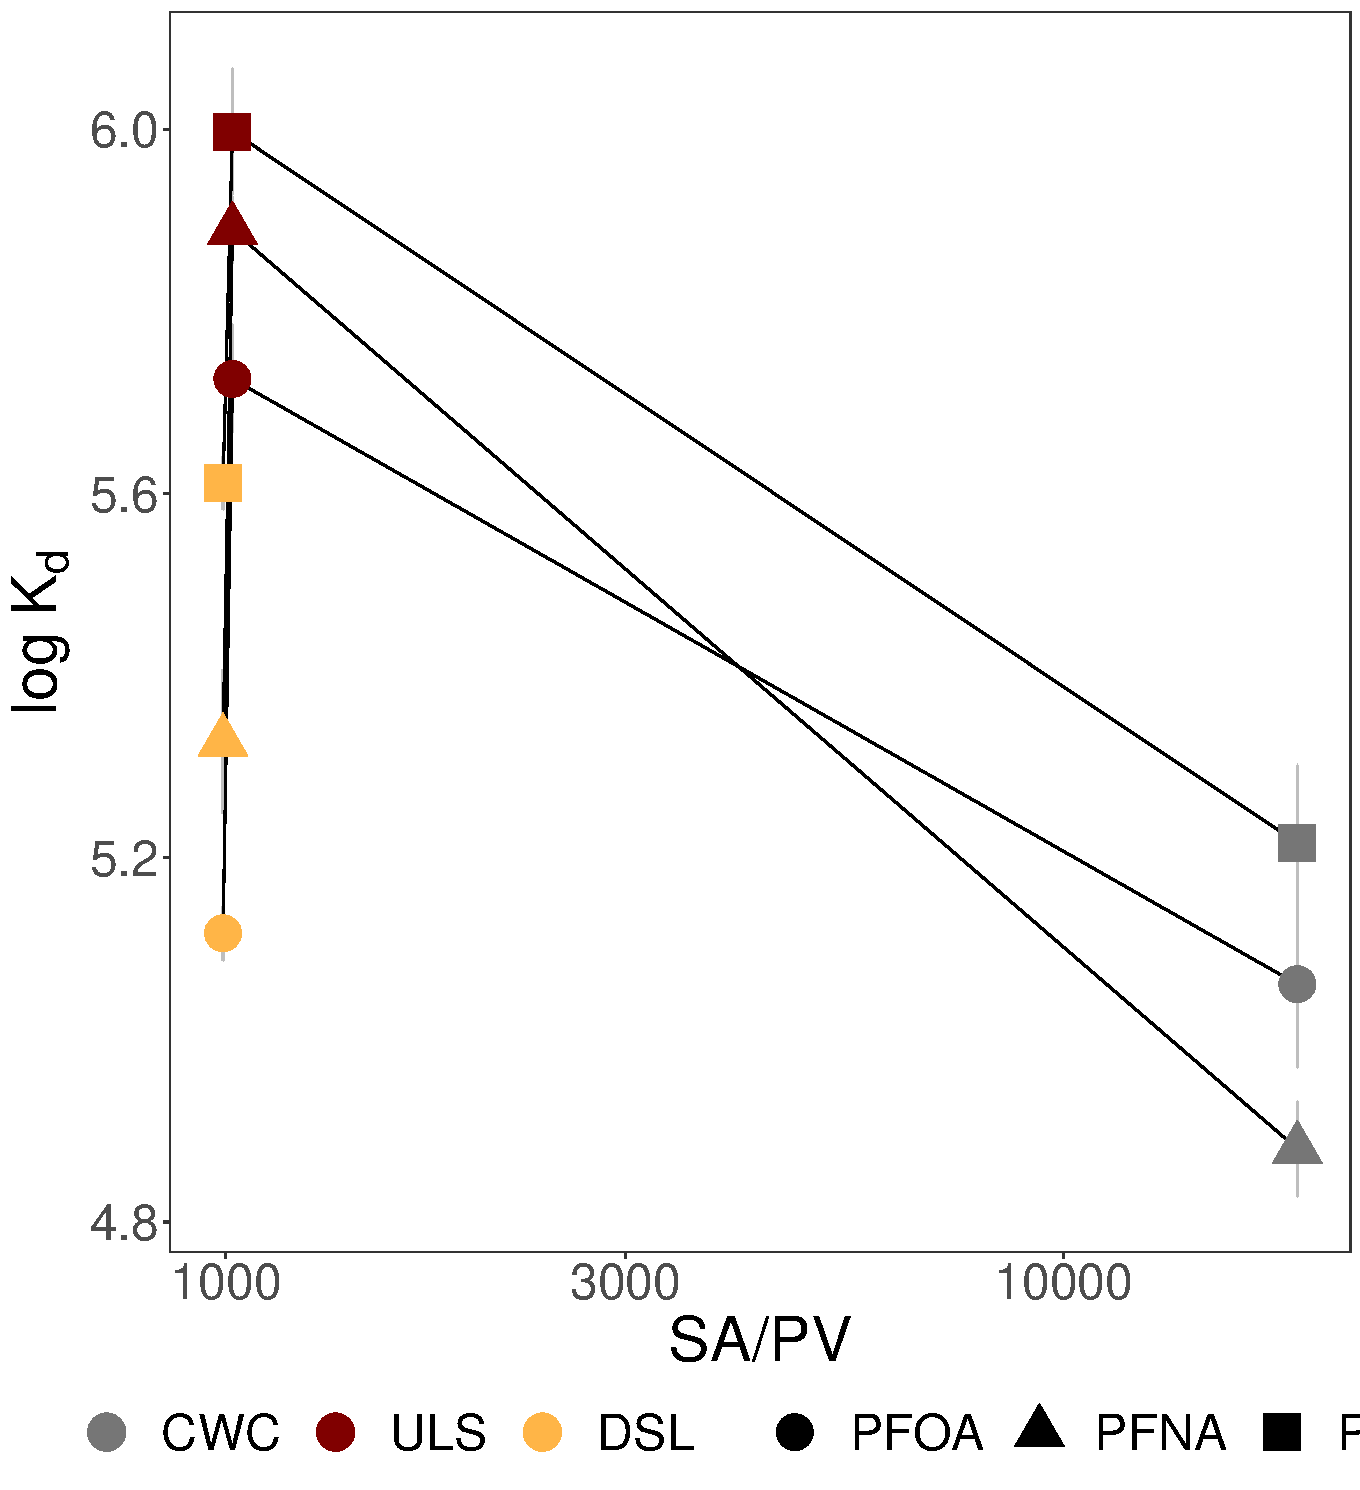
\includegraphics[width=0.3\textwidth]{R/figs/Kd_1ugL_SA_PV.pdf}
}
\hfill
\subfloat[\label{subfig:Kd_SAPVC}]{%
  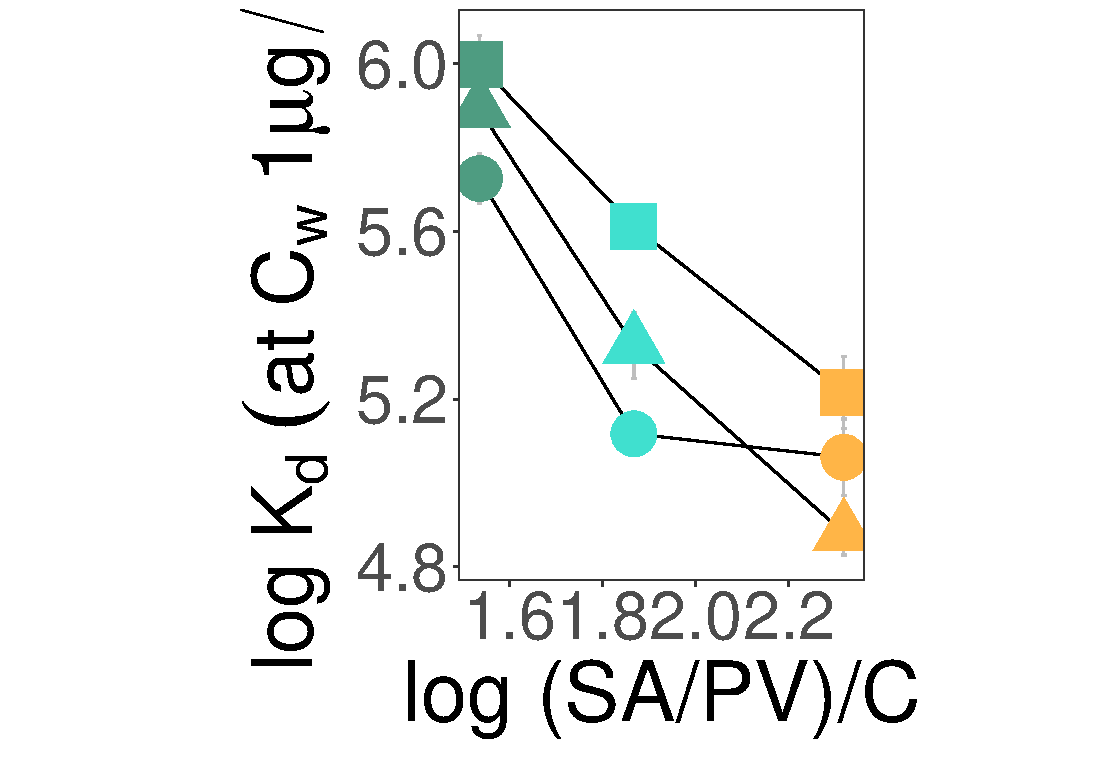
\includegraphics[width=0.3\textwidth]{R/figs/Kd_1ugL_SA_PV_C.pdf}
}
\caption{The correlation of $log~K_d$ vs. (a) log C (b) log SA/PV (c) log (SA/PV)/C using BET for SA and BJH for PV by biomass feedstock. Error bars are the propagated standard error.}
\label{fig:Kd_SAPV_C}
\end{figure}

\begin{figure}[!ht]
\subfloat[\label{subfig:Kd_Ca}]{%
  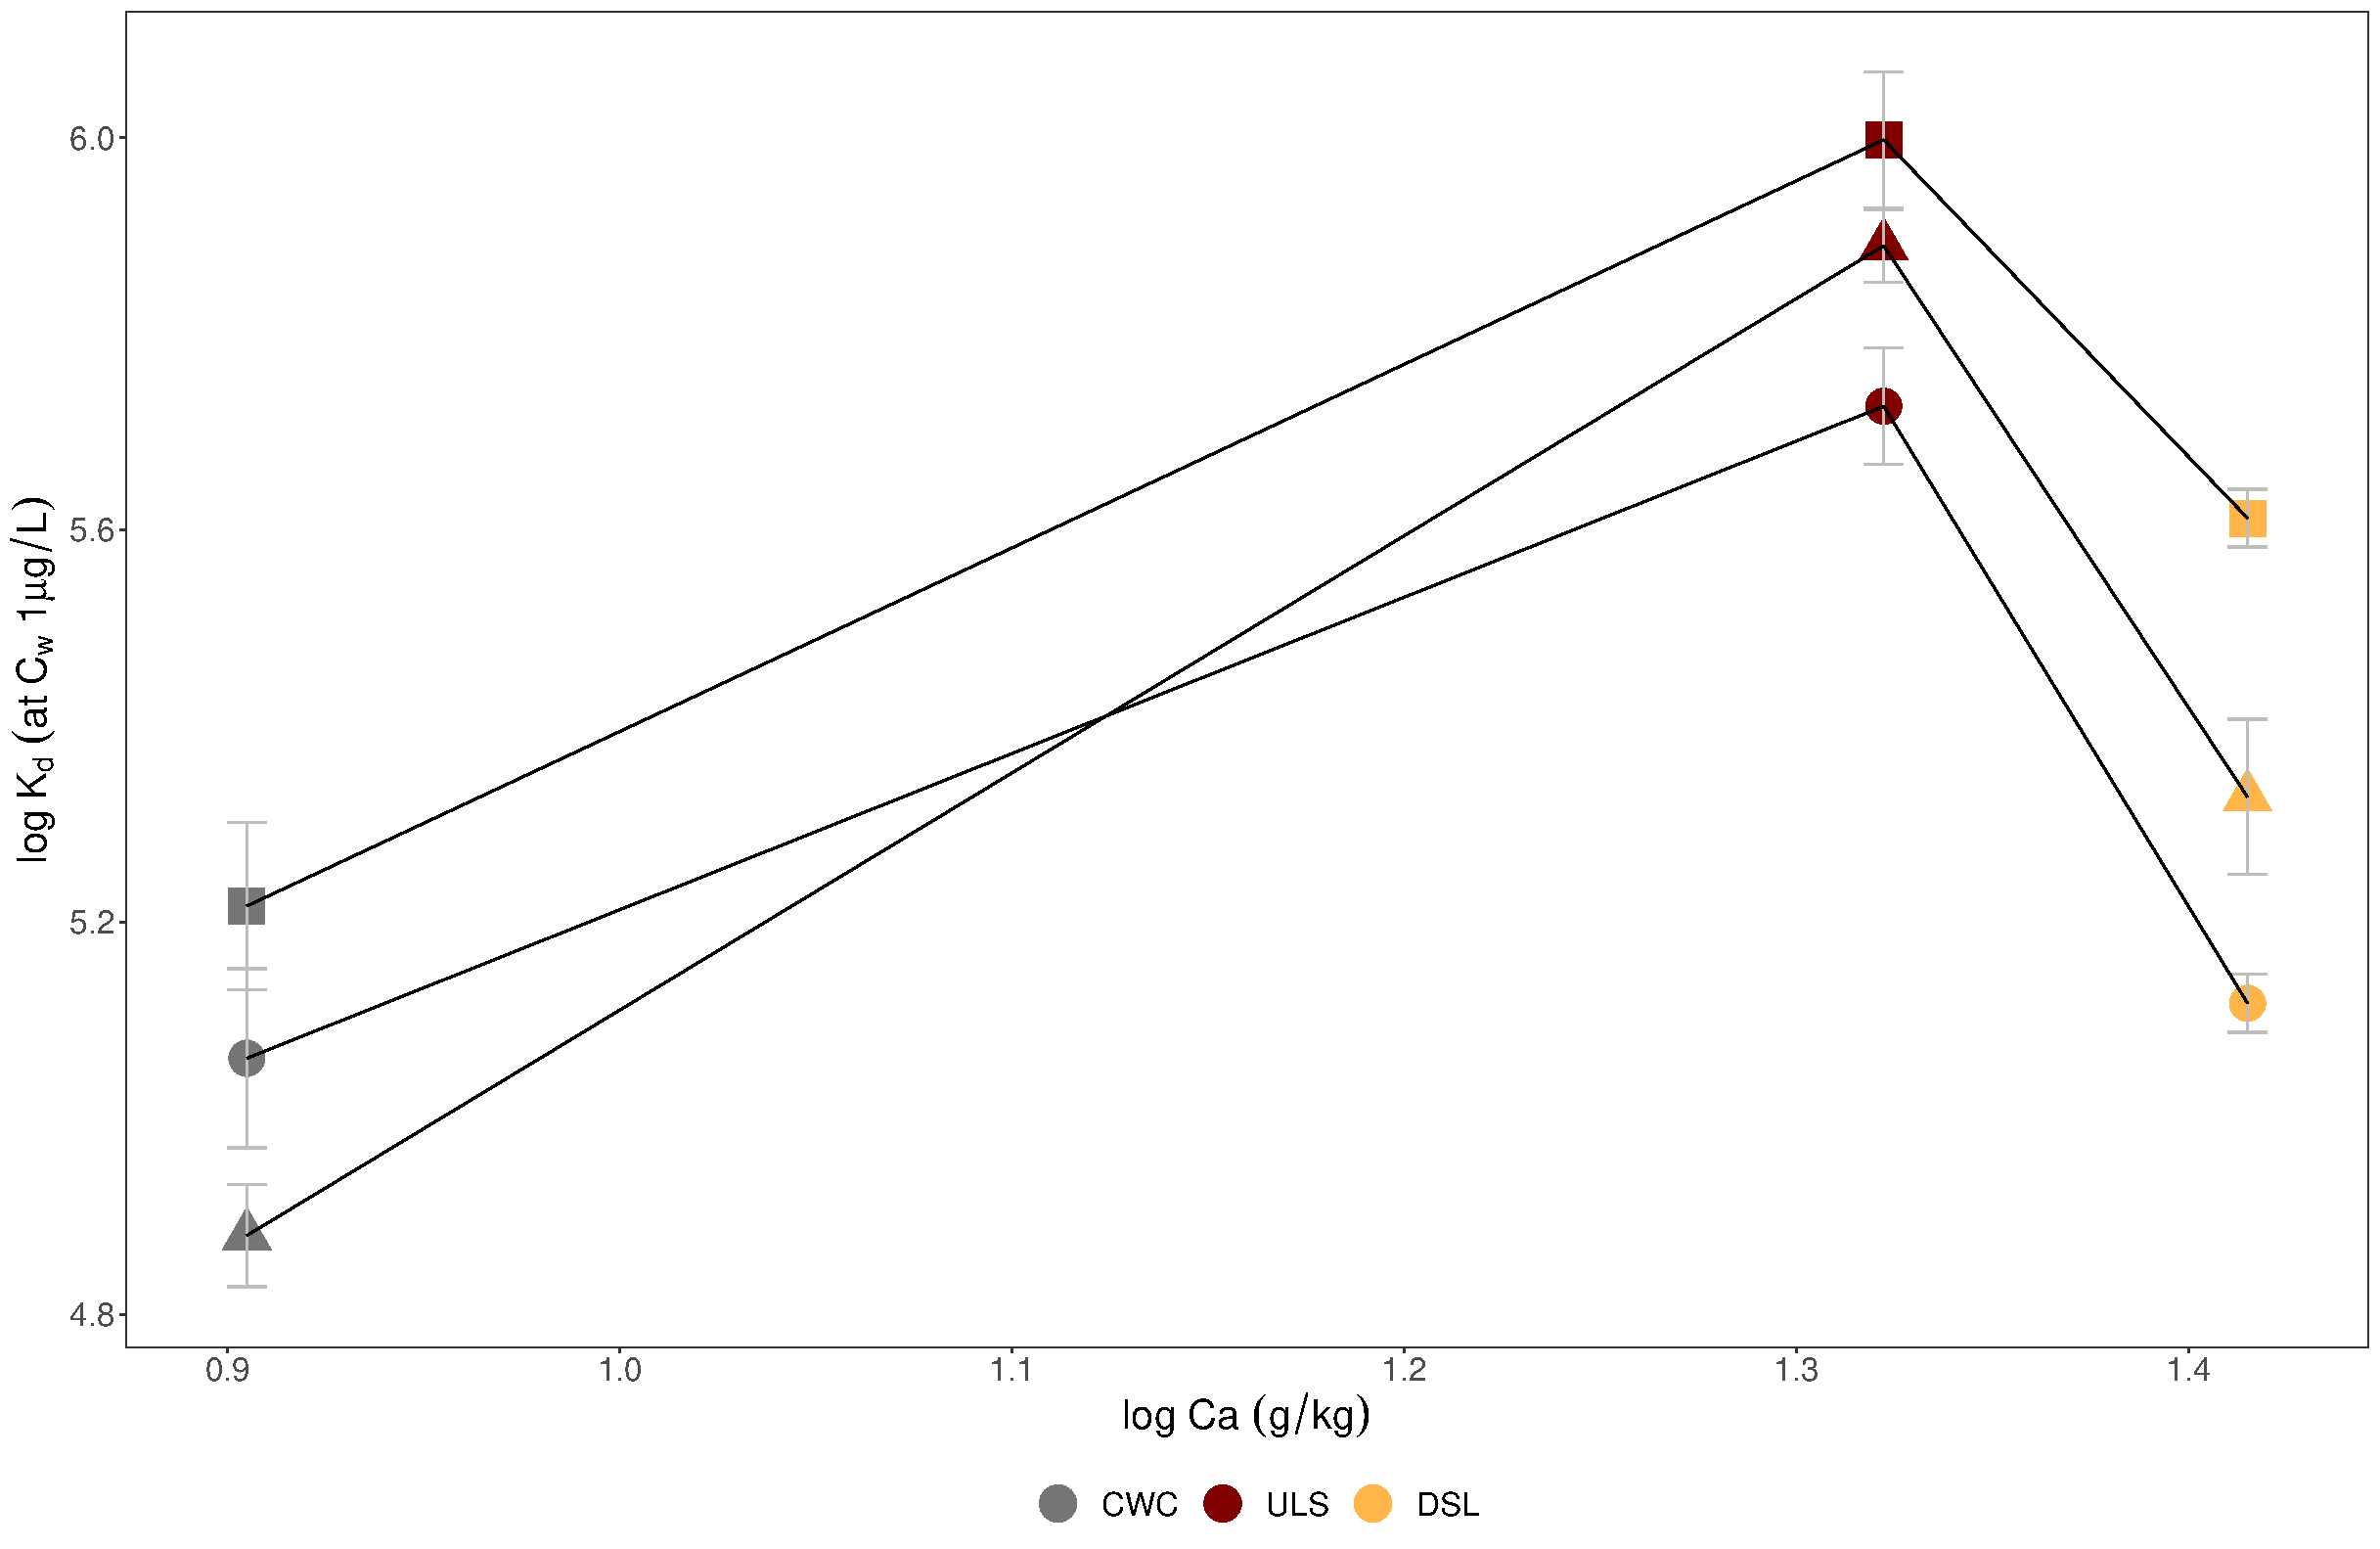
\includegraphics[width=0.45\textwidth]{R/figs/Kd_1ugL_Ca.pdf}
}
\hfill
\subfloat[\label{subfig:Kd_PV}]{%
  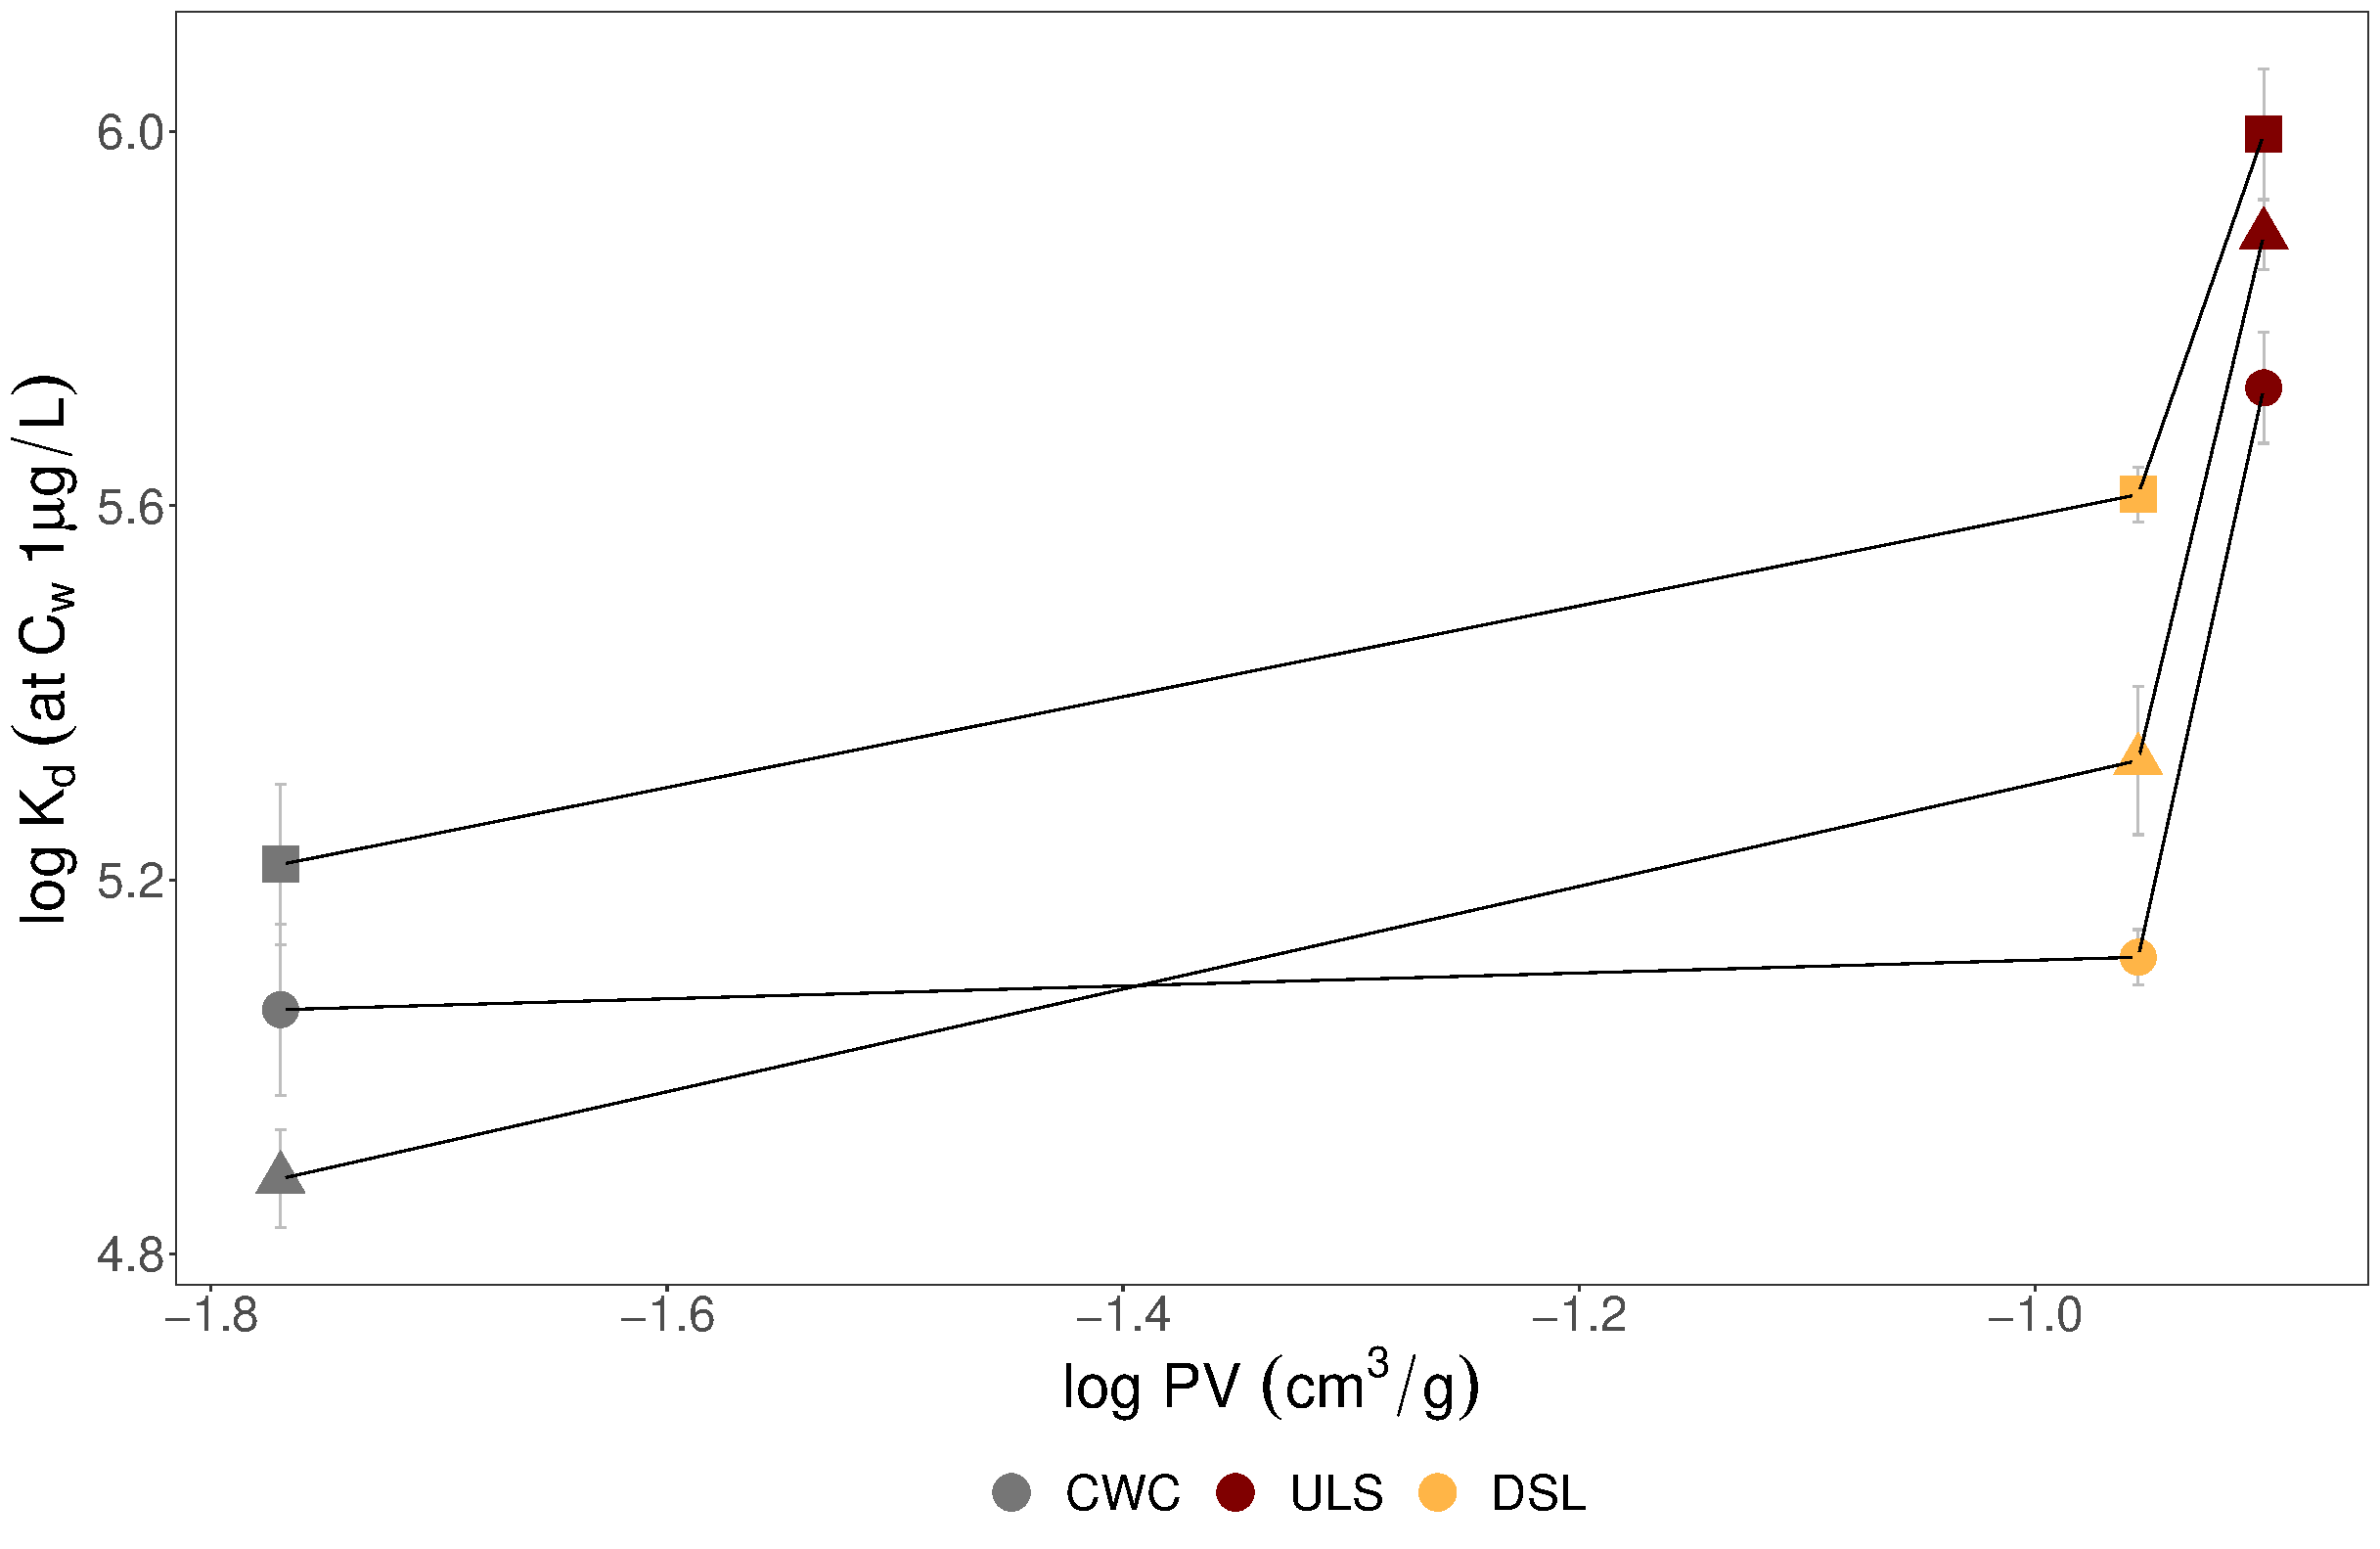
\includegraphics[width=0.45\textwidth]{R/figs/Kd_1ugL_PVN2.pdf}
}
\hfill
\subfloat[\label{subfig:Kd_PV_Ca}]{%
  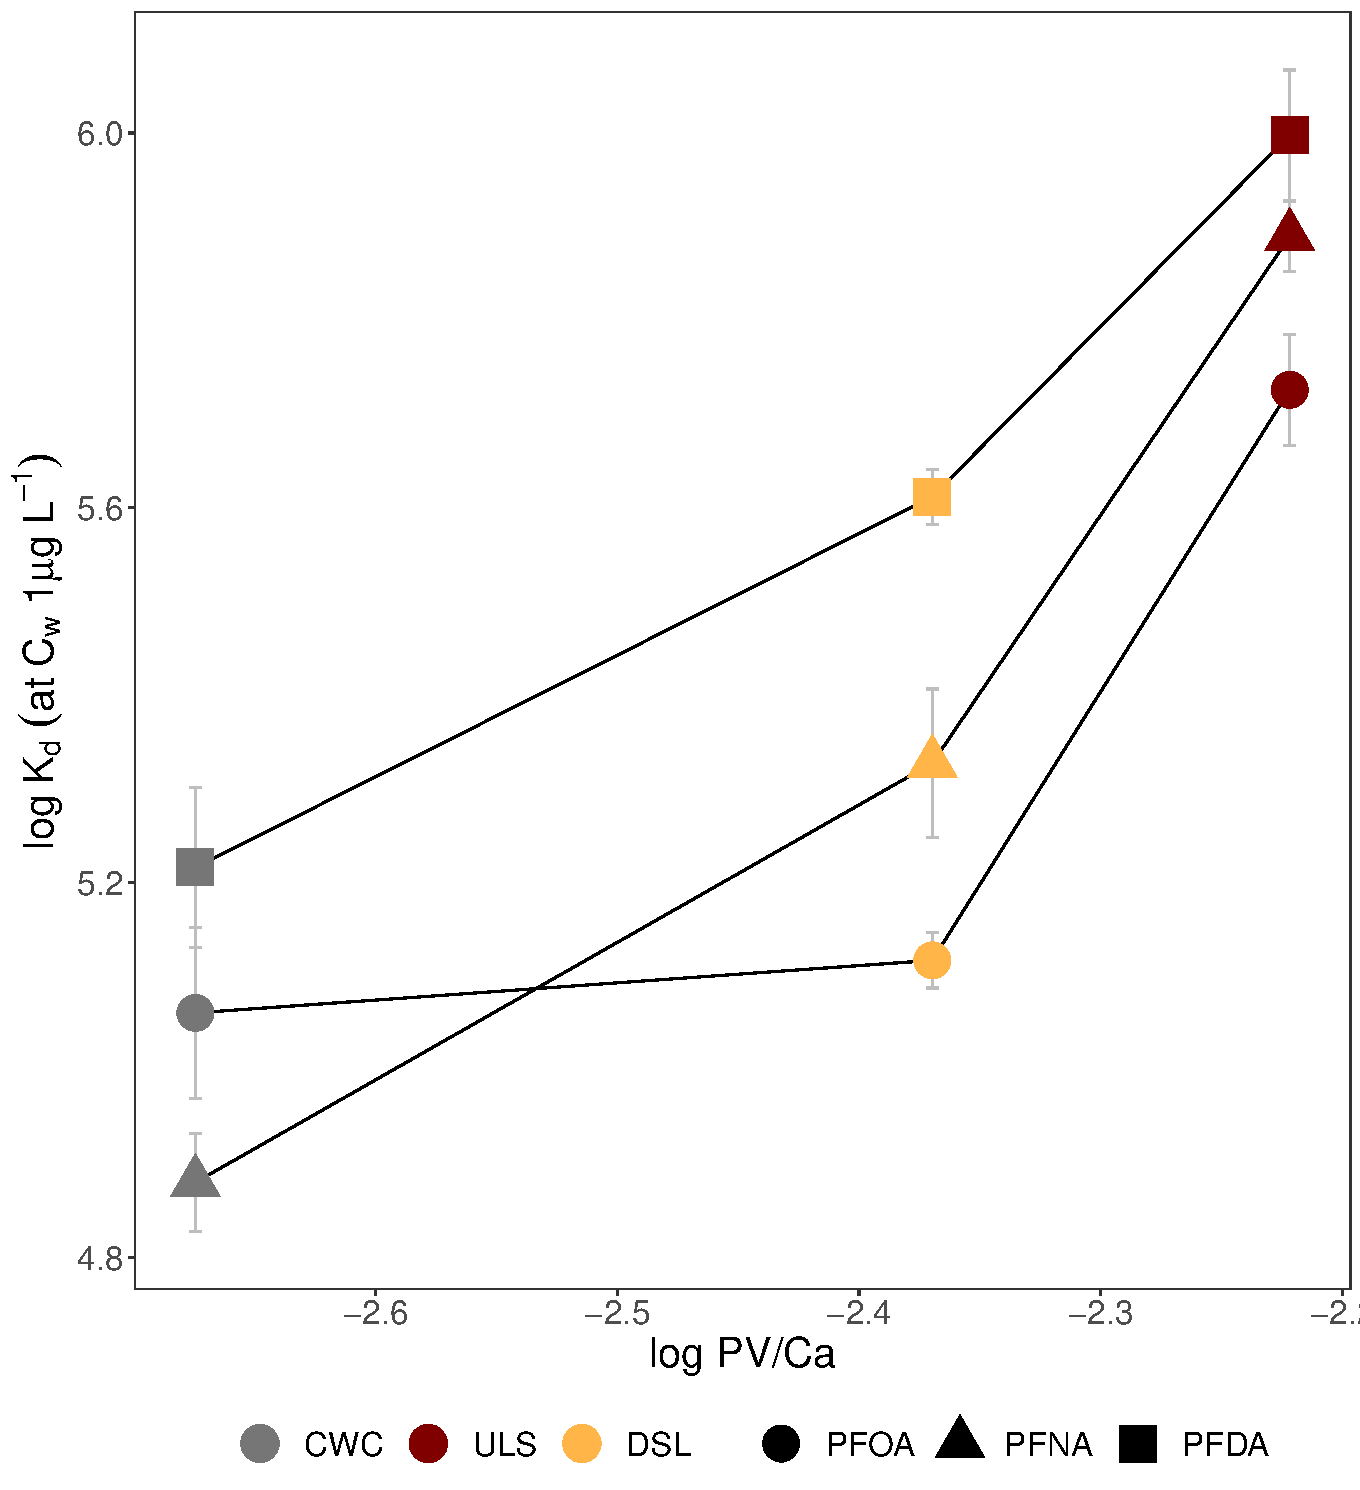
\includegraphics[width=0.45\textwidth]{R/figs/Kd_1ugL_PVN2_Ca.pdf}
}
\hfill
\subfloat[\label{subfig:Kd_SAPVCa}]{%
  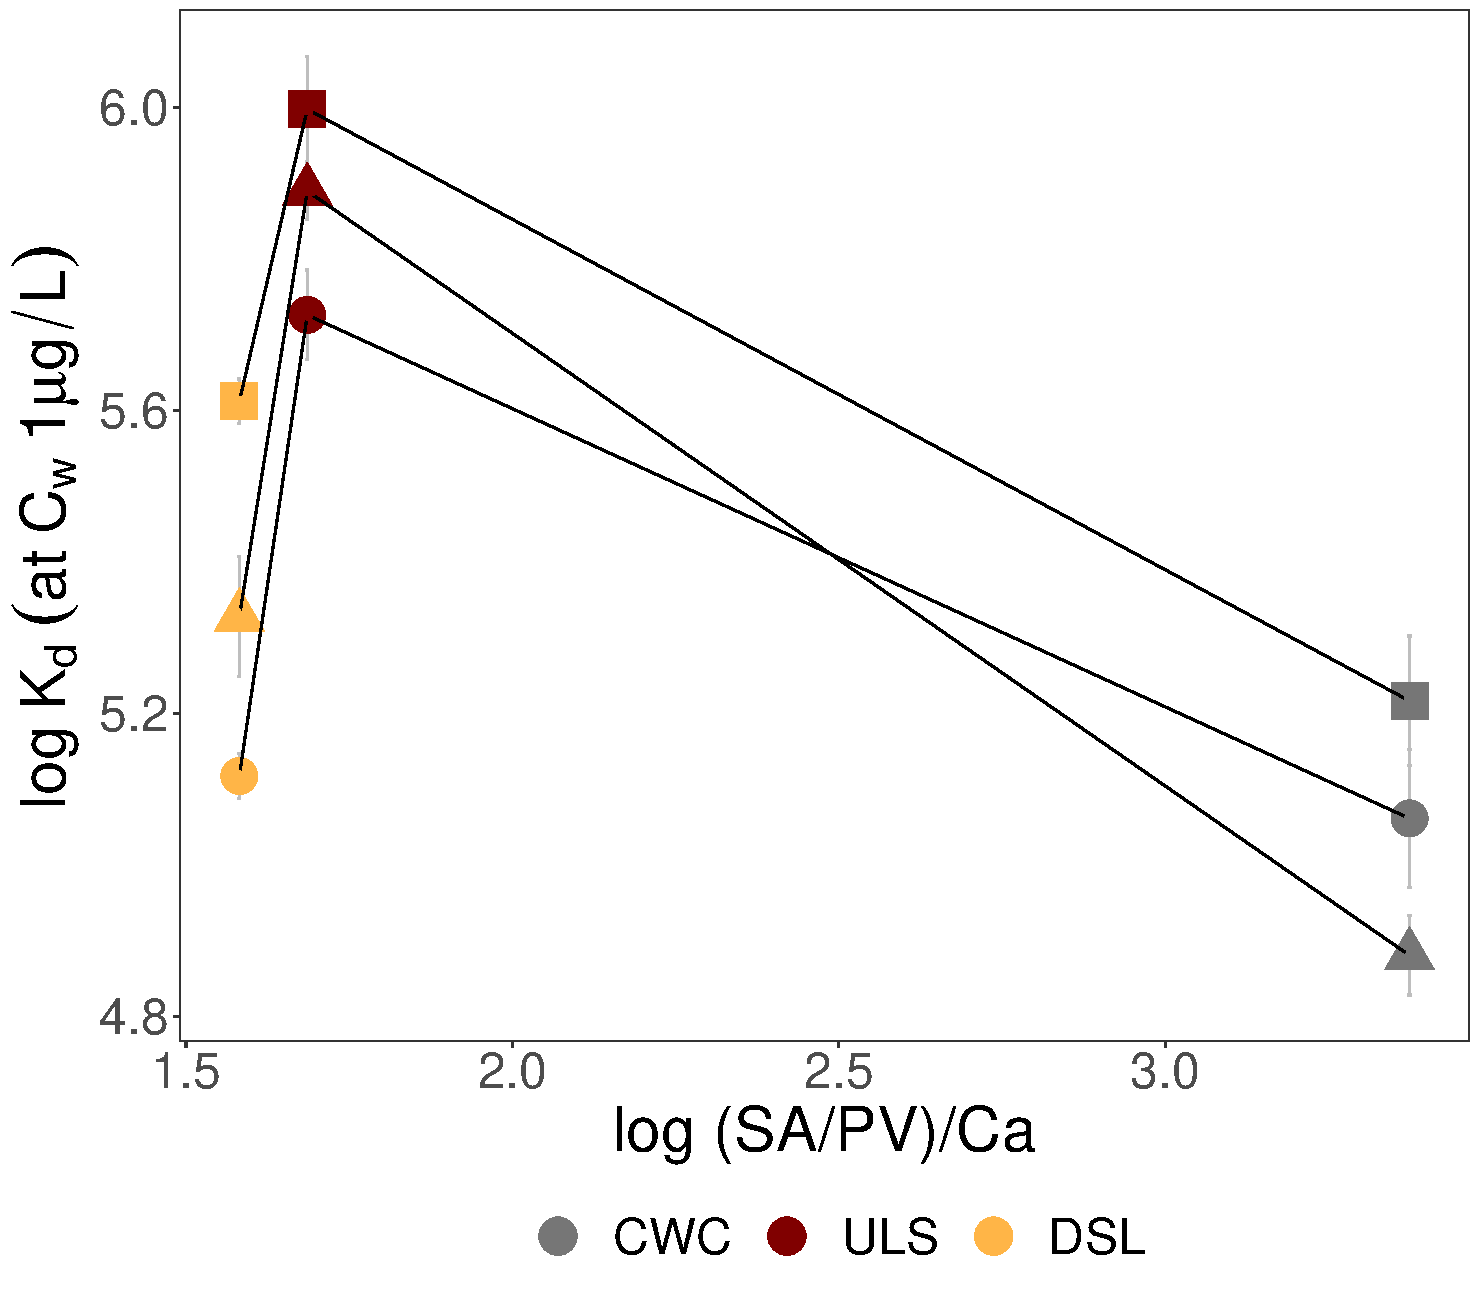
\includegraphics[width=0.45\textwidth]{R/figs/Kd_1ugL_SA_PV_Ca.pdf}
}
\caption{The correlation of $log~K_d$ vs. (a) log Ca (b) log PV (c) log PV/Ca (d) log (SA/PV)/Ca using BET for SA and BJH for PV by biomass feedstock. Error bars are the propagated standard error.}
\label{fig:Kd_SAPV_Ca}
\end{figure}

\begin{figure}[!ht]
\subfloat[\label{subfig:SA_small}]{%
  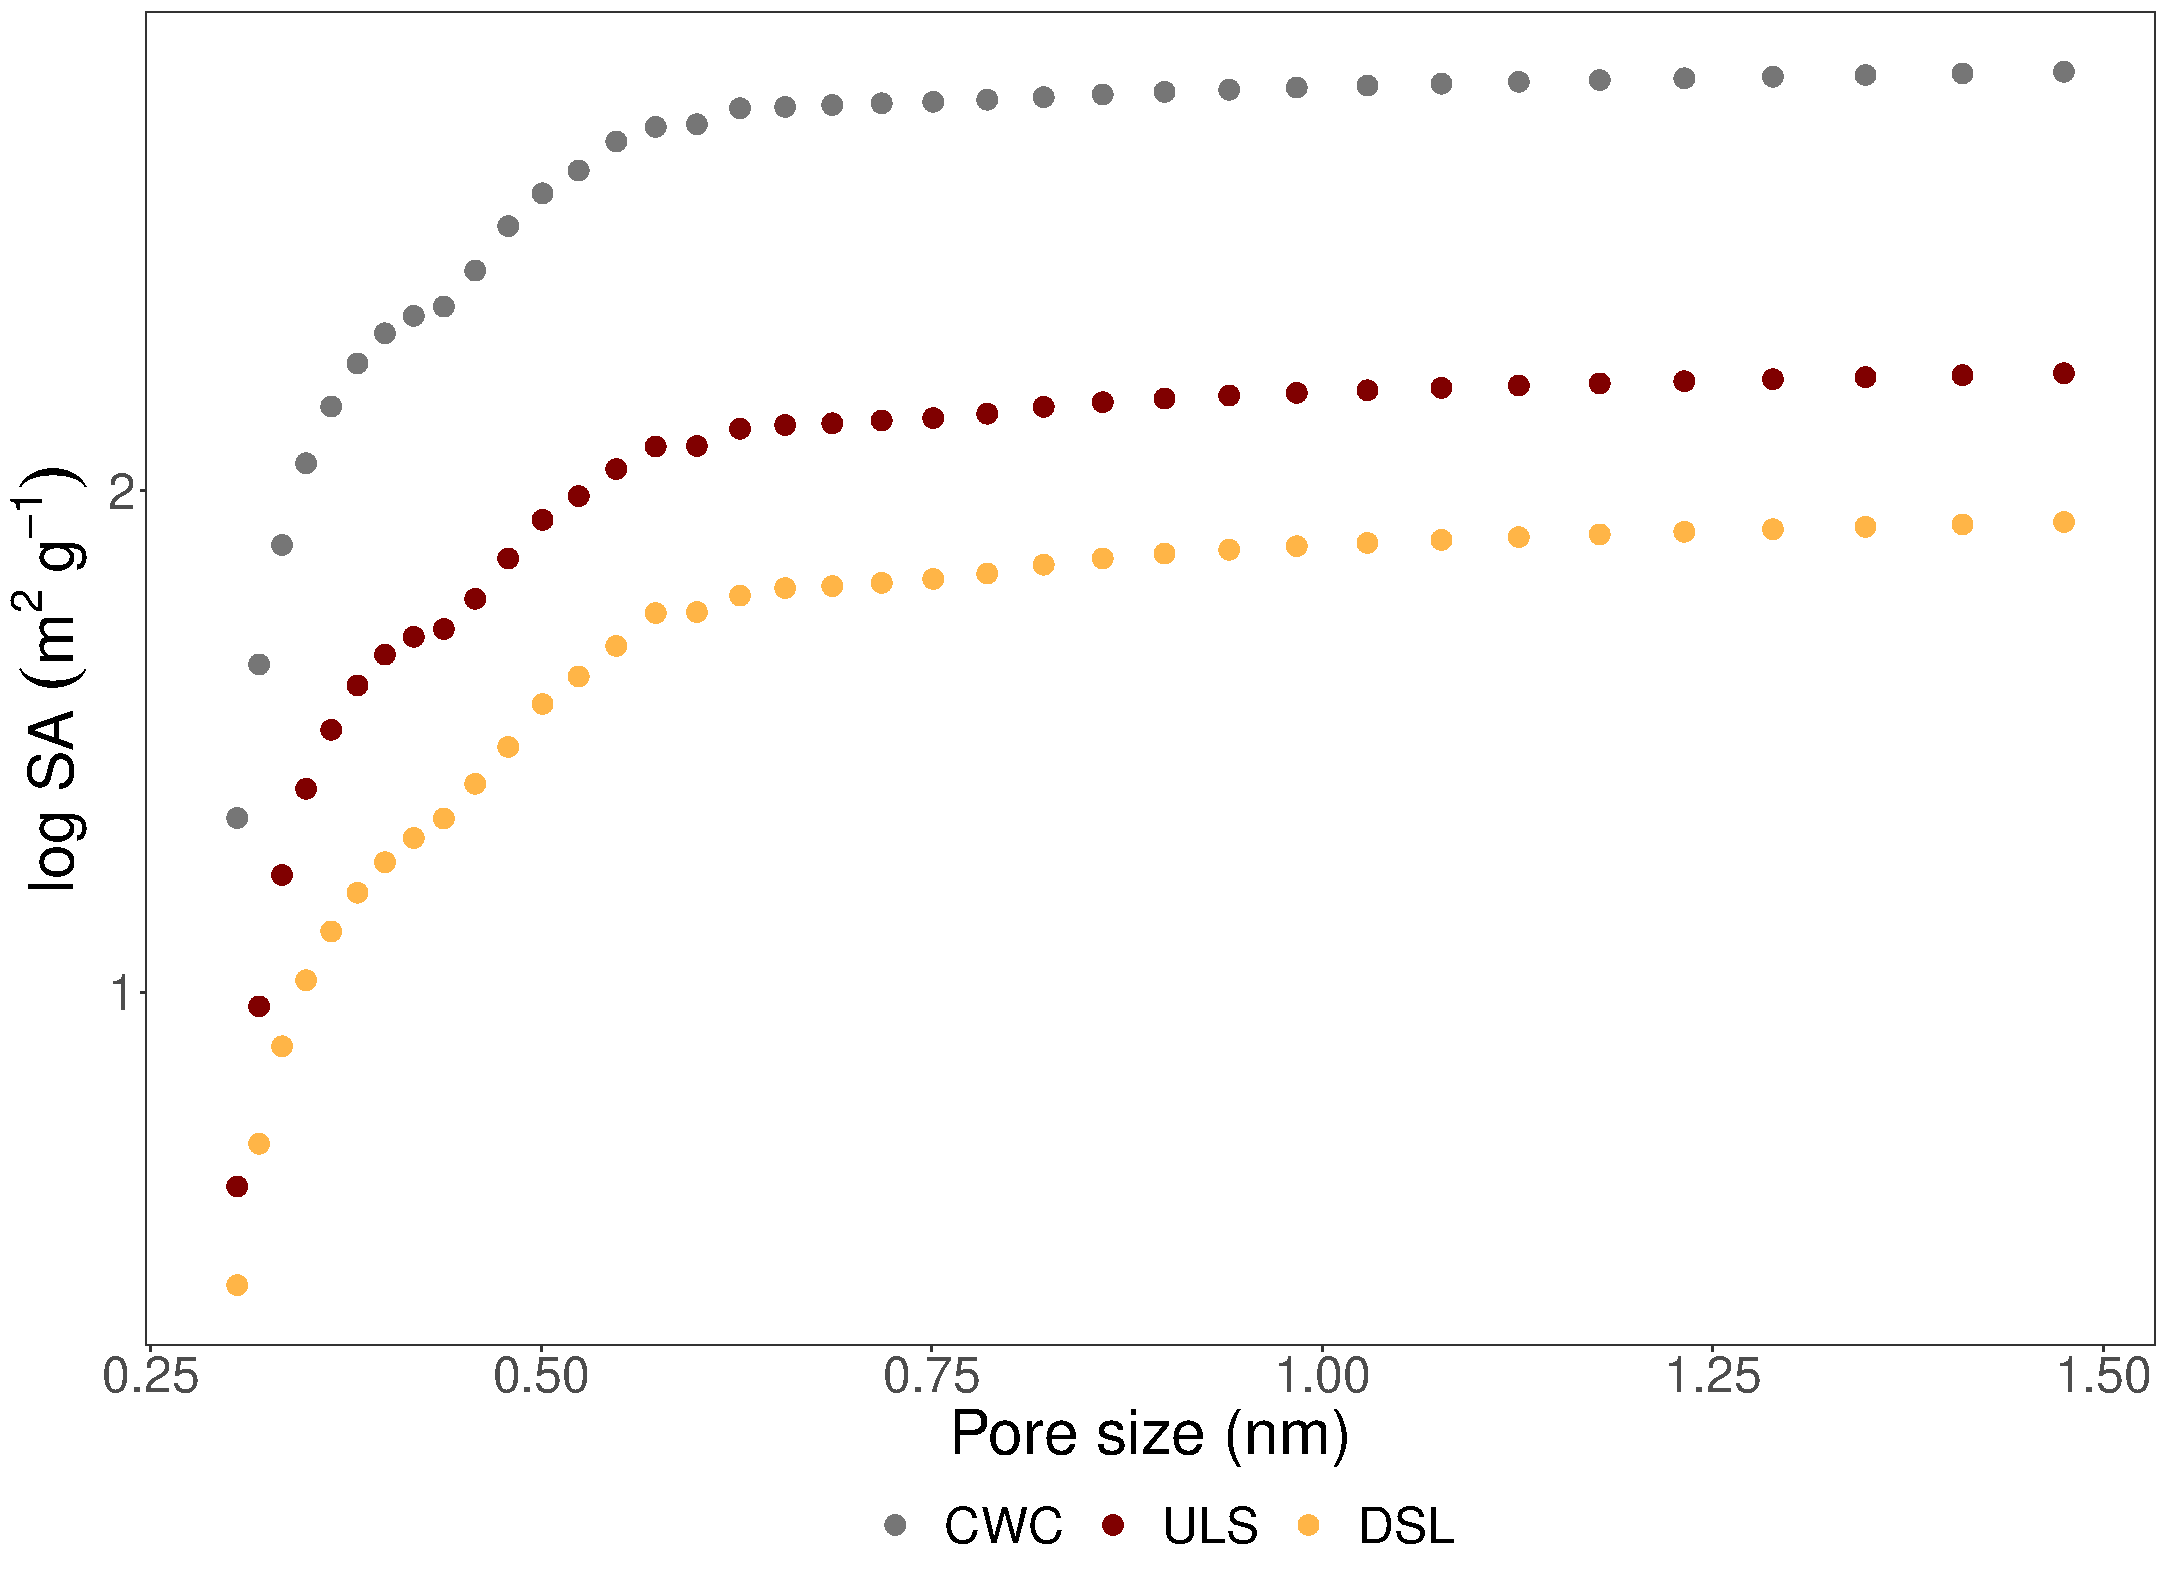
\includegraphics[width=0.31\textwidth]{R/figs/SA_small.pdf}
}
\hfill
\subfloat[\label{subfig:PV_small}]{%
  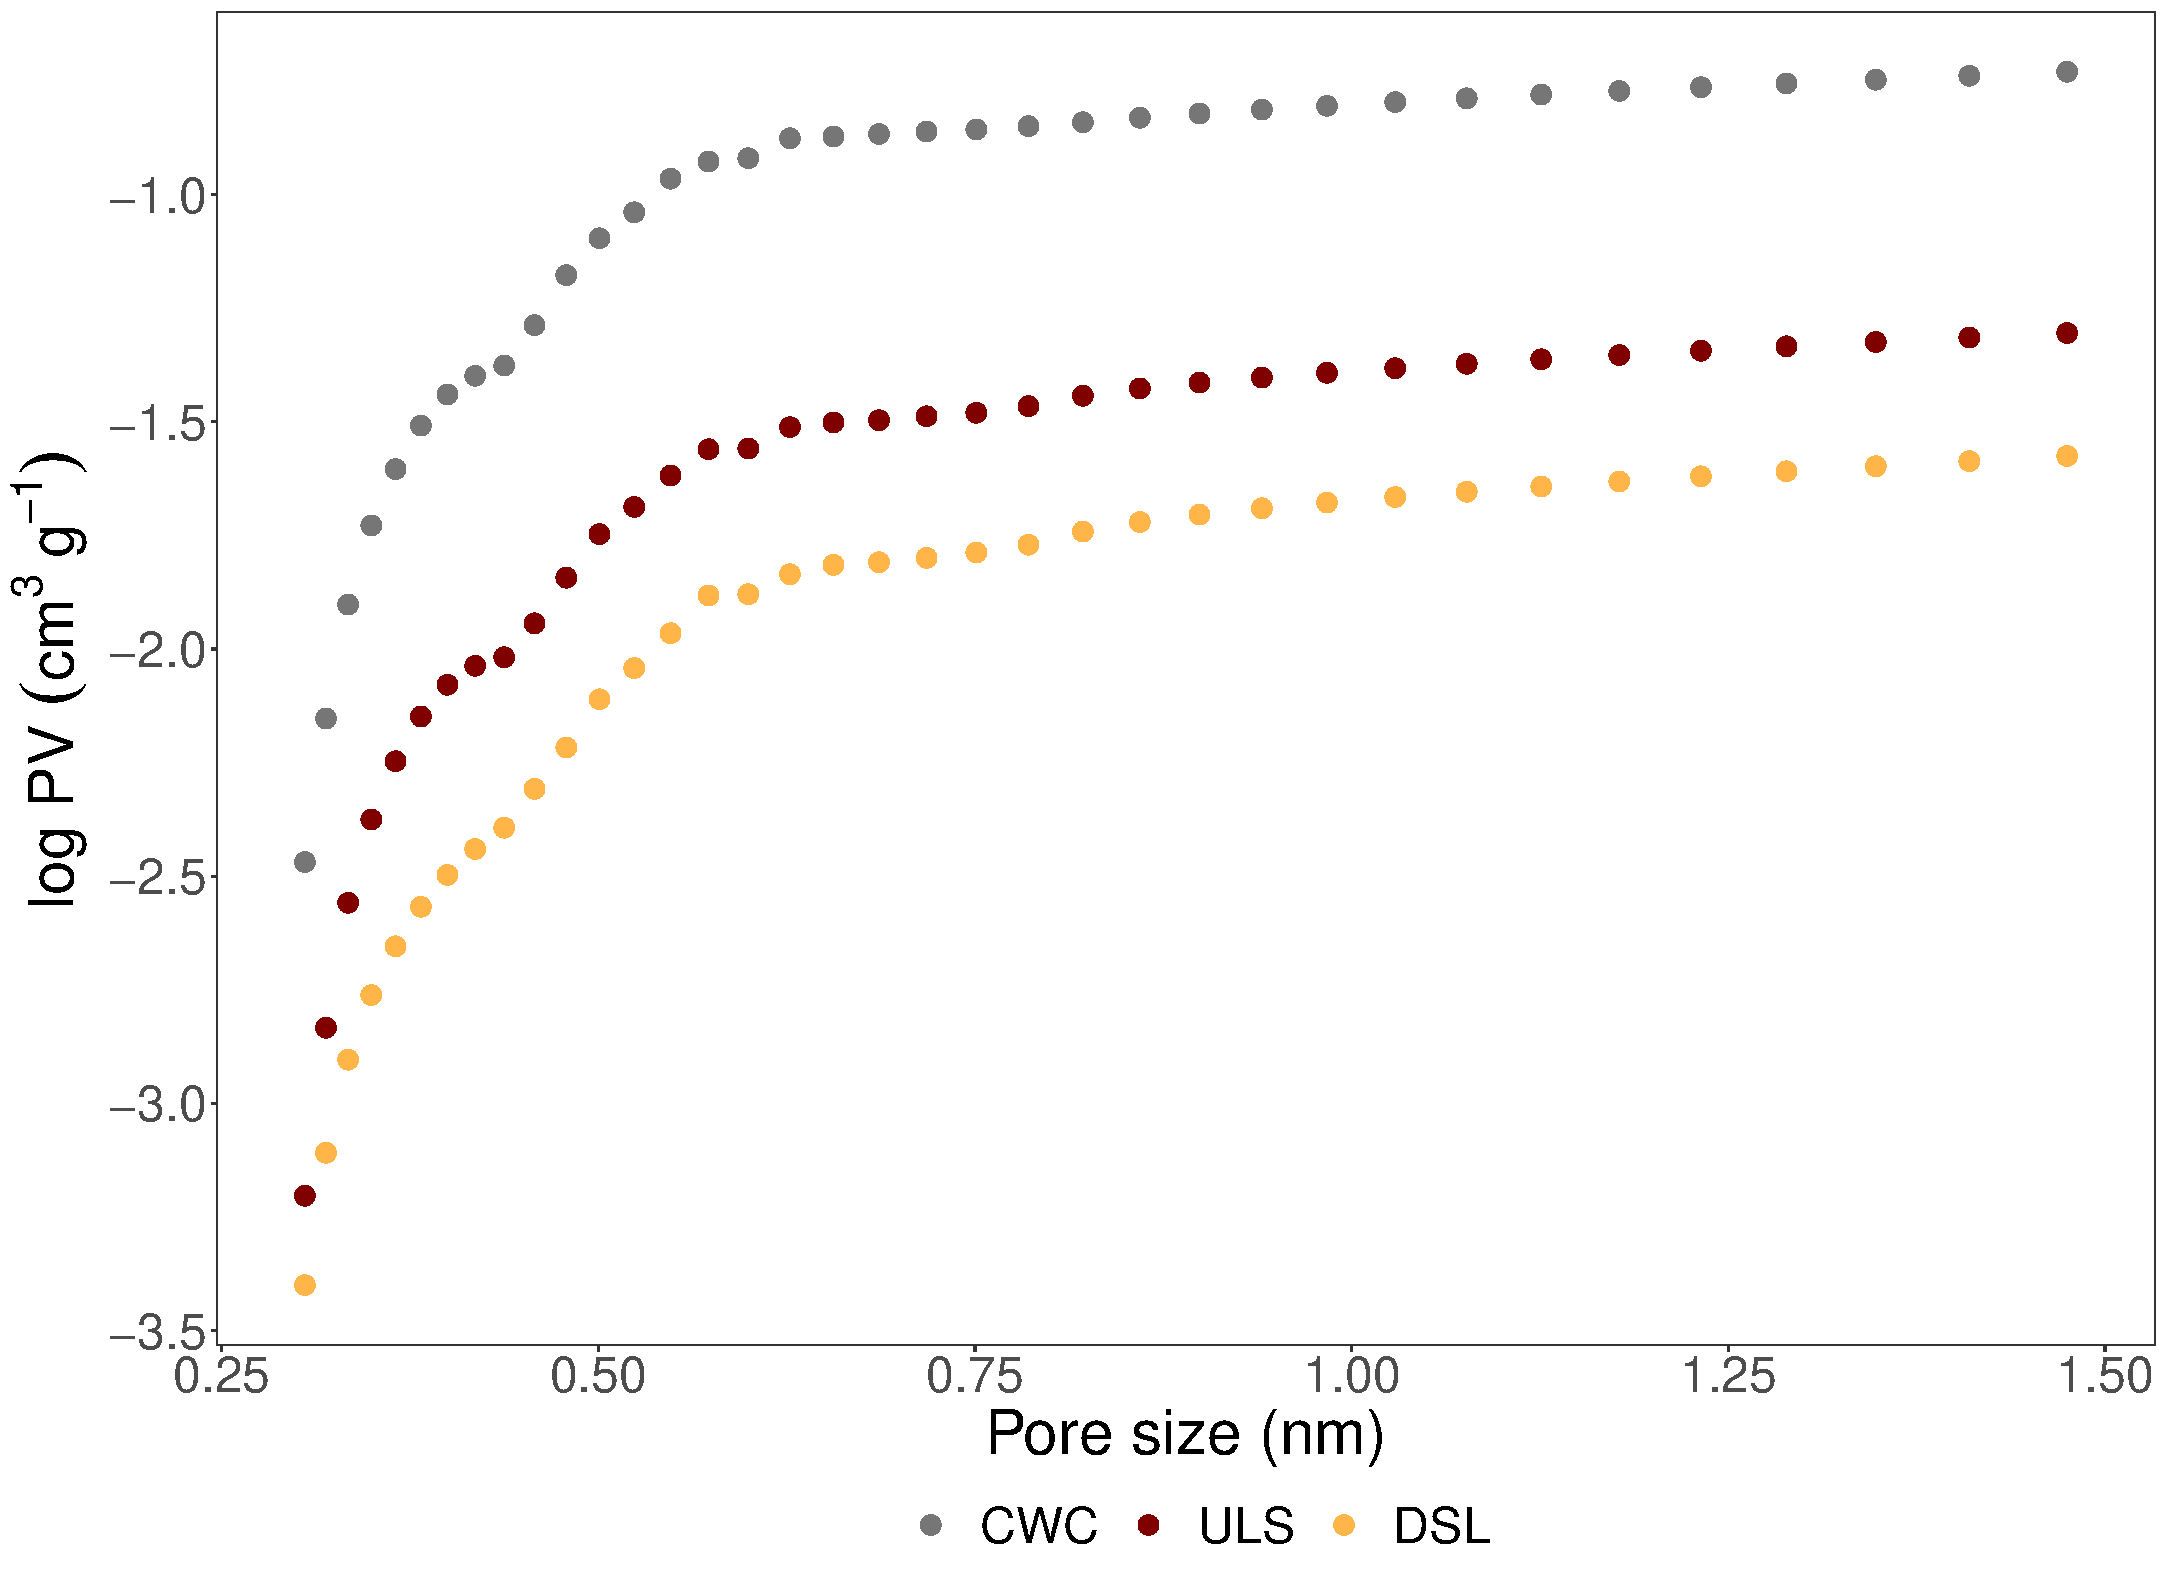
\includegraphics[width=0.31\textwidth]{R/figs/PV_small.pdf}
}
\hfill
\subfloat[\label{subfig:SAPV_small}]{%
  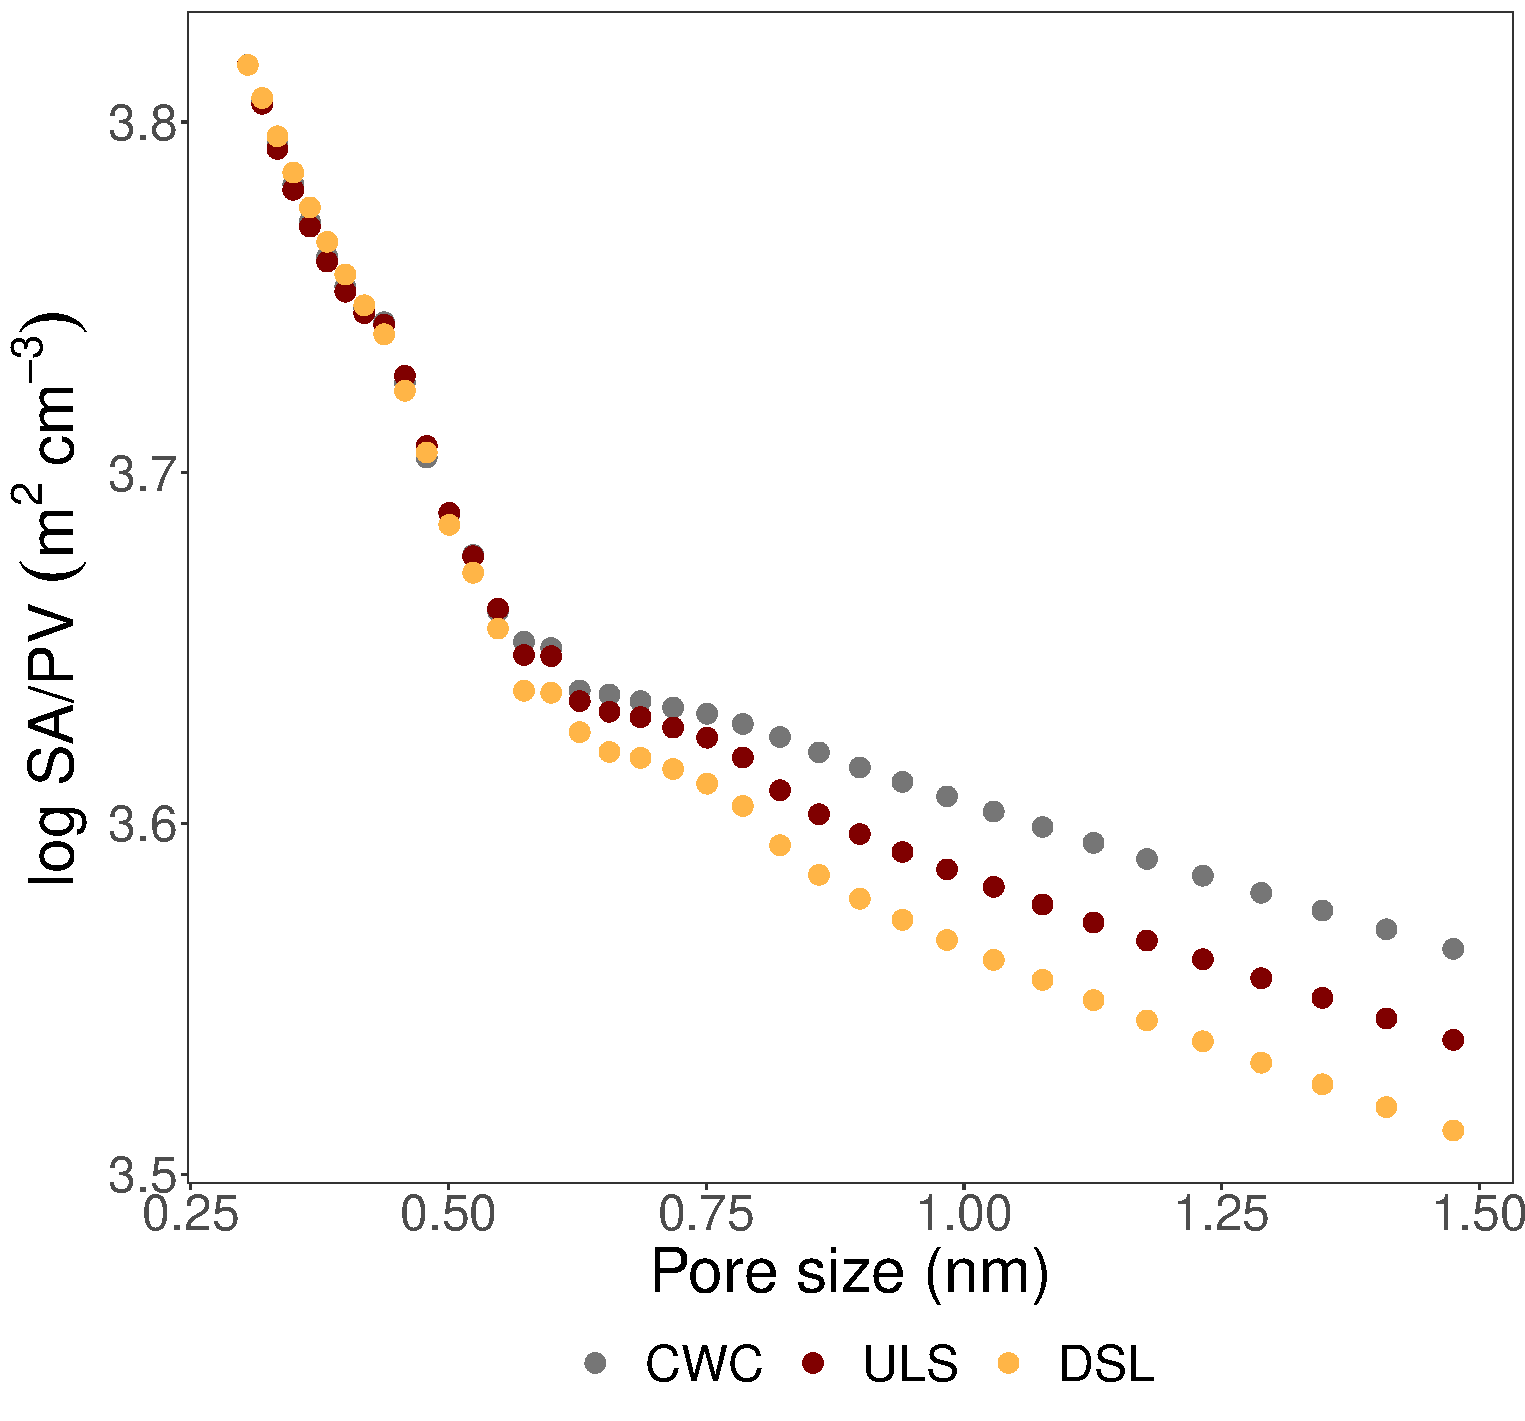
\includegraphics[width=0.31\textwidth]{R/figs/SAPV_small.pdf}
}
\caption{Cumulative pore size distribution for pores 0.4-1.5 nm using DFT.}
\label{fig:PZD_small}
\end{figure}

\begin{figure}[!ht]
\subfloat[\label{subfig:SA_large}]{%
  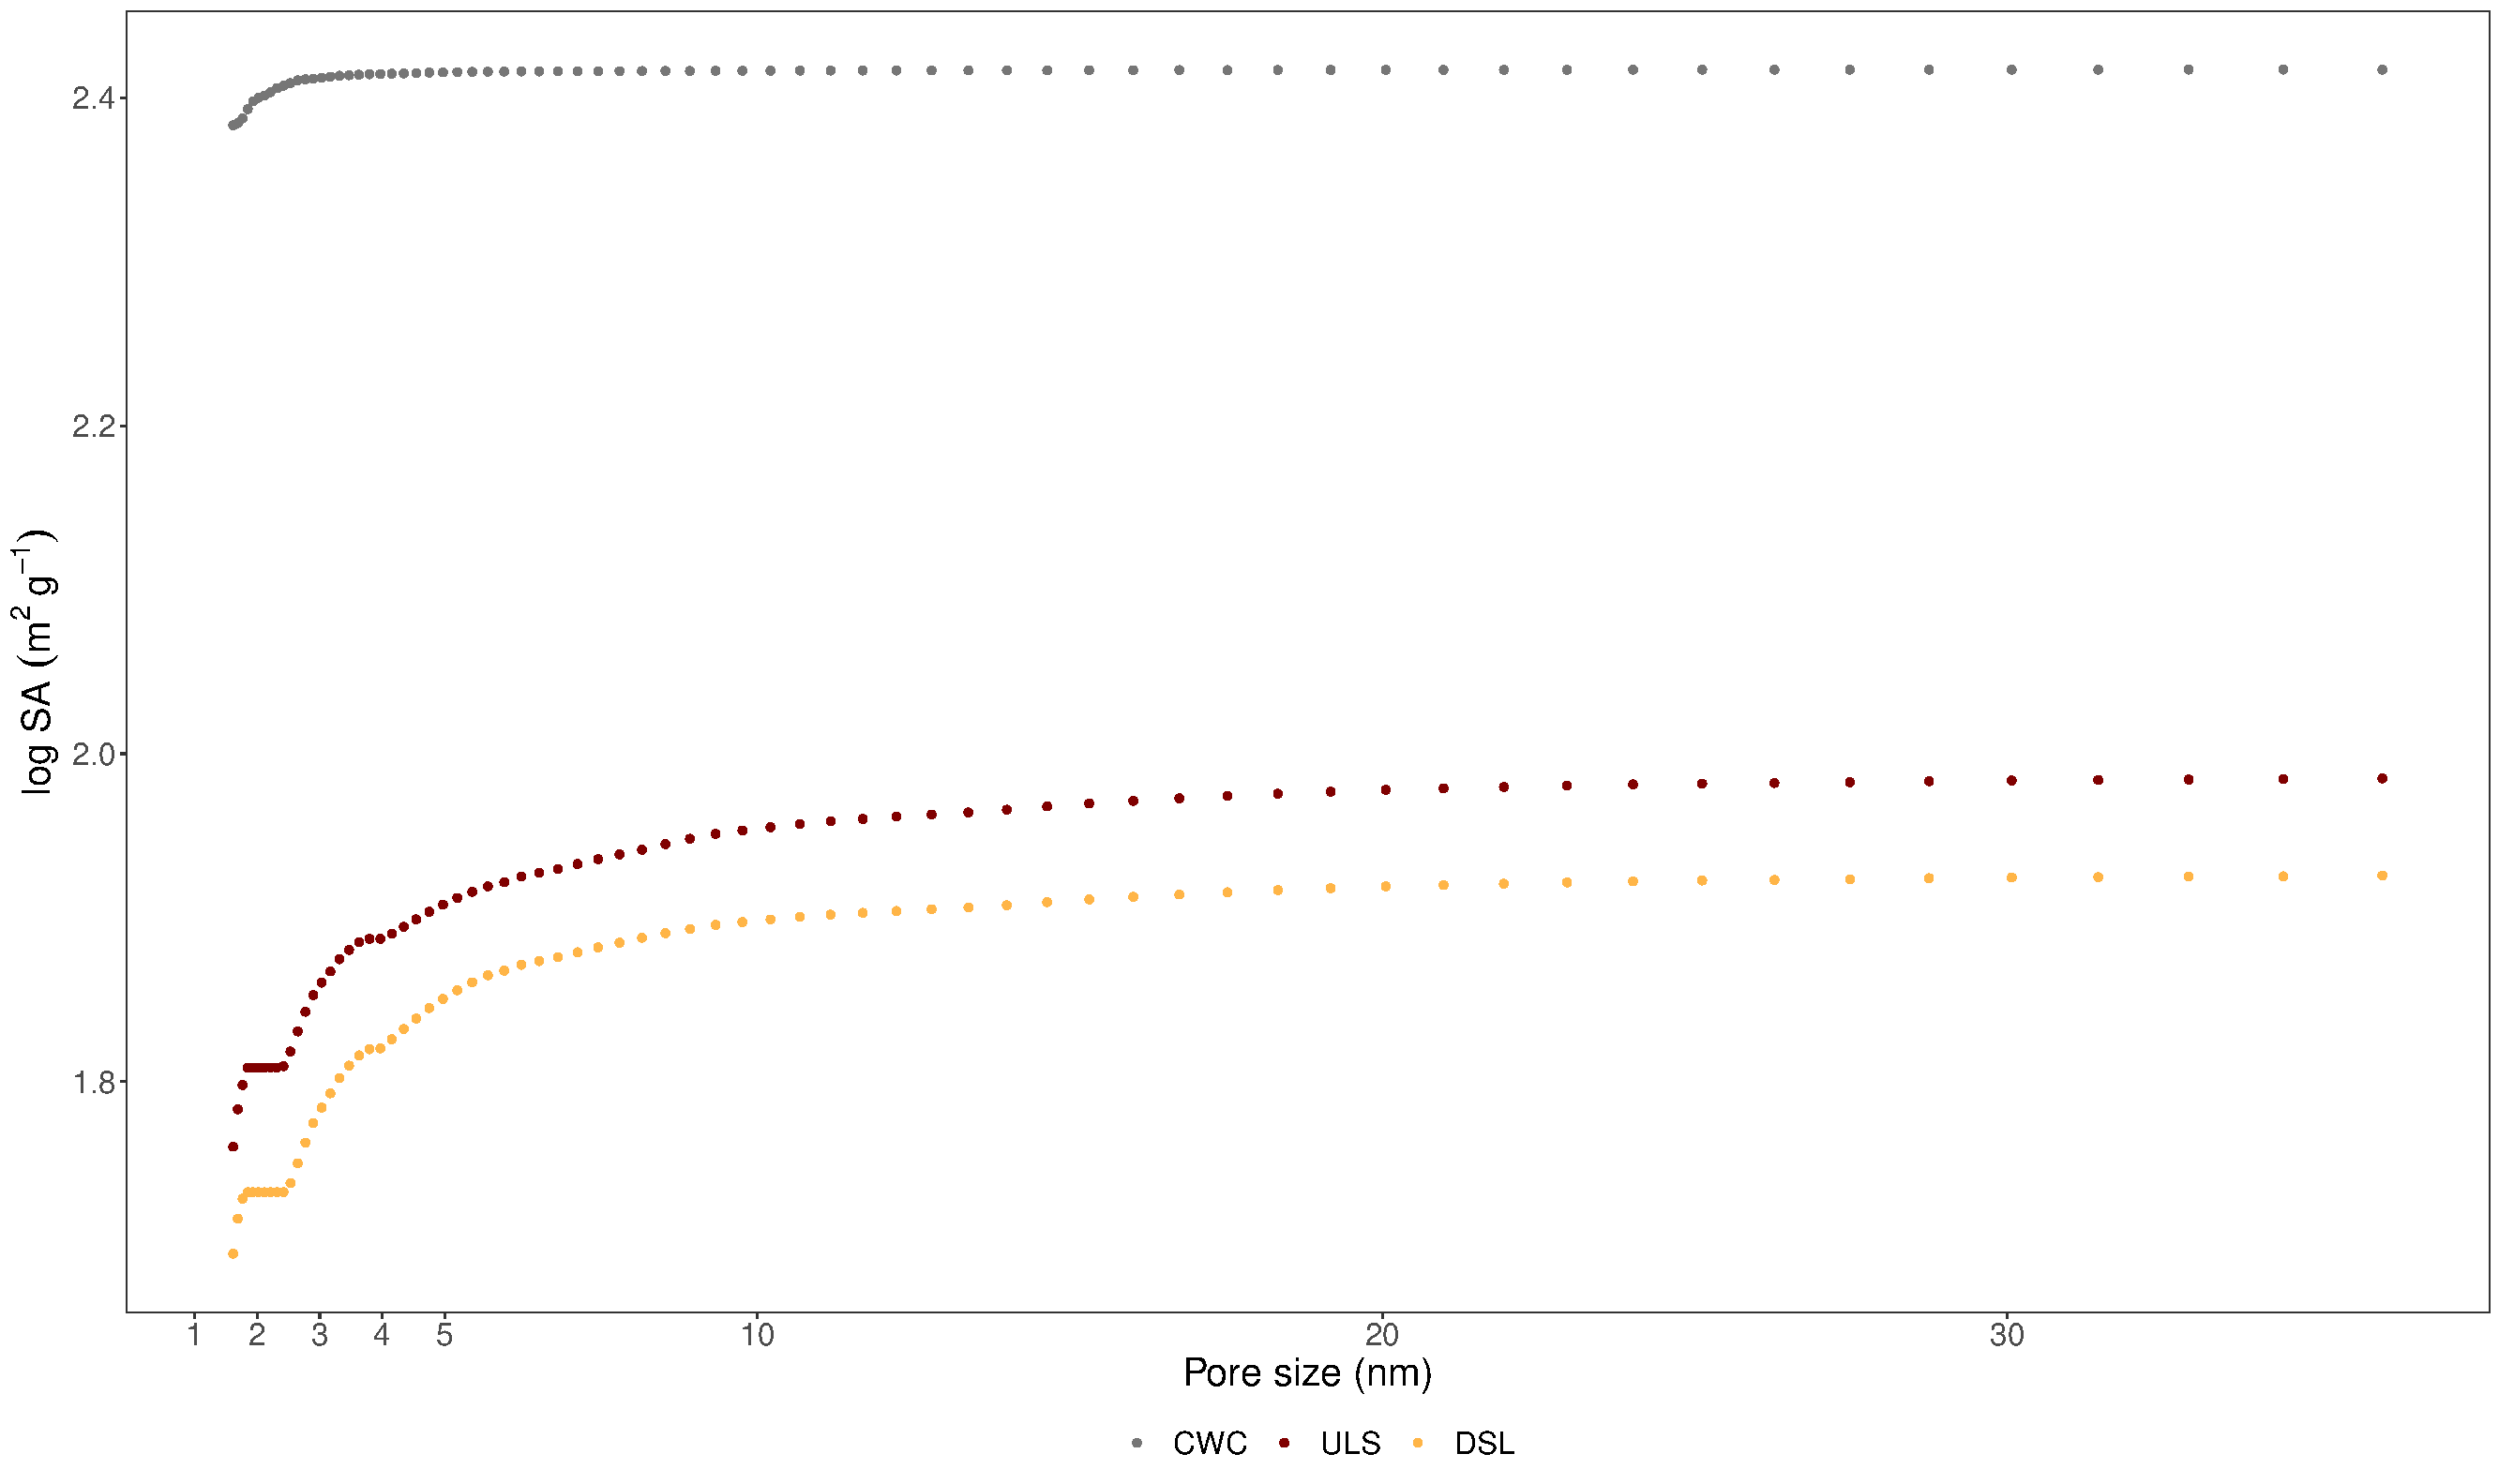
\includegraphics[width=0.45\textwidth]{R/figs/SA_large.pdf}
}
\hfill
\subfloat[\label{subfig:PV_large}]{%
  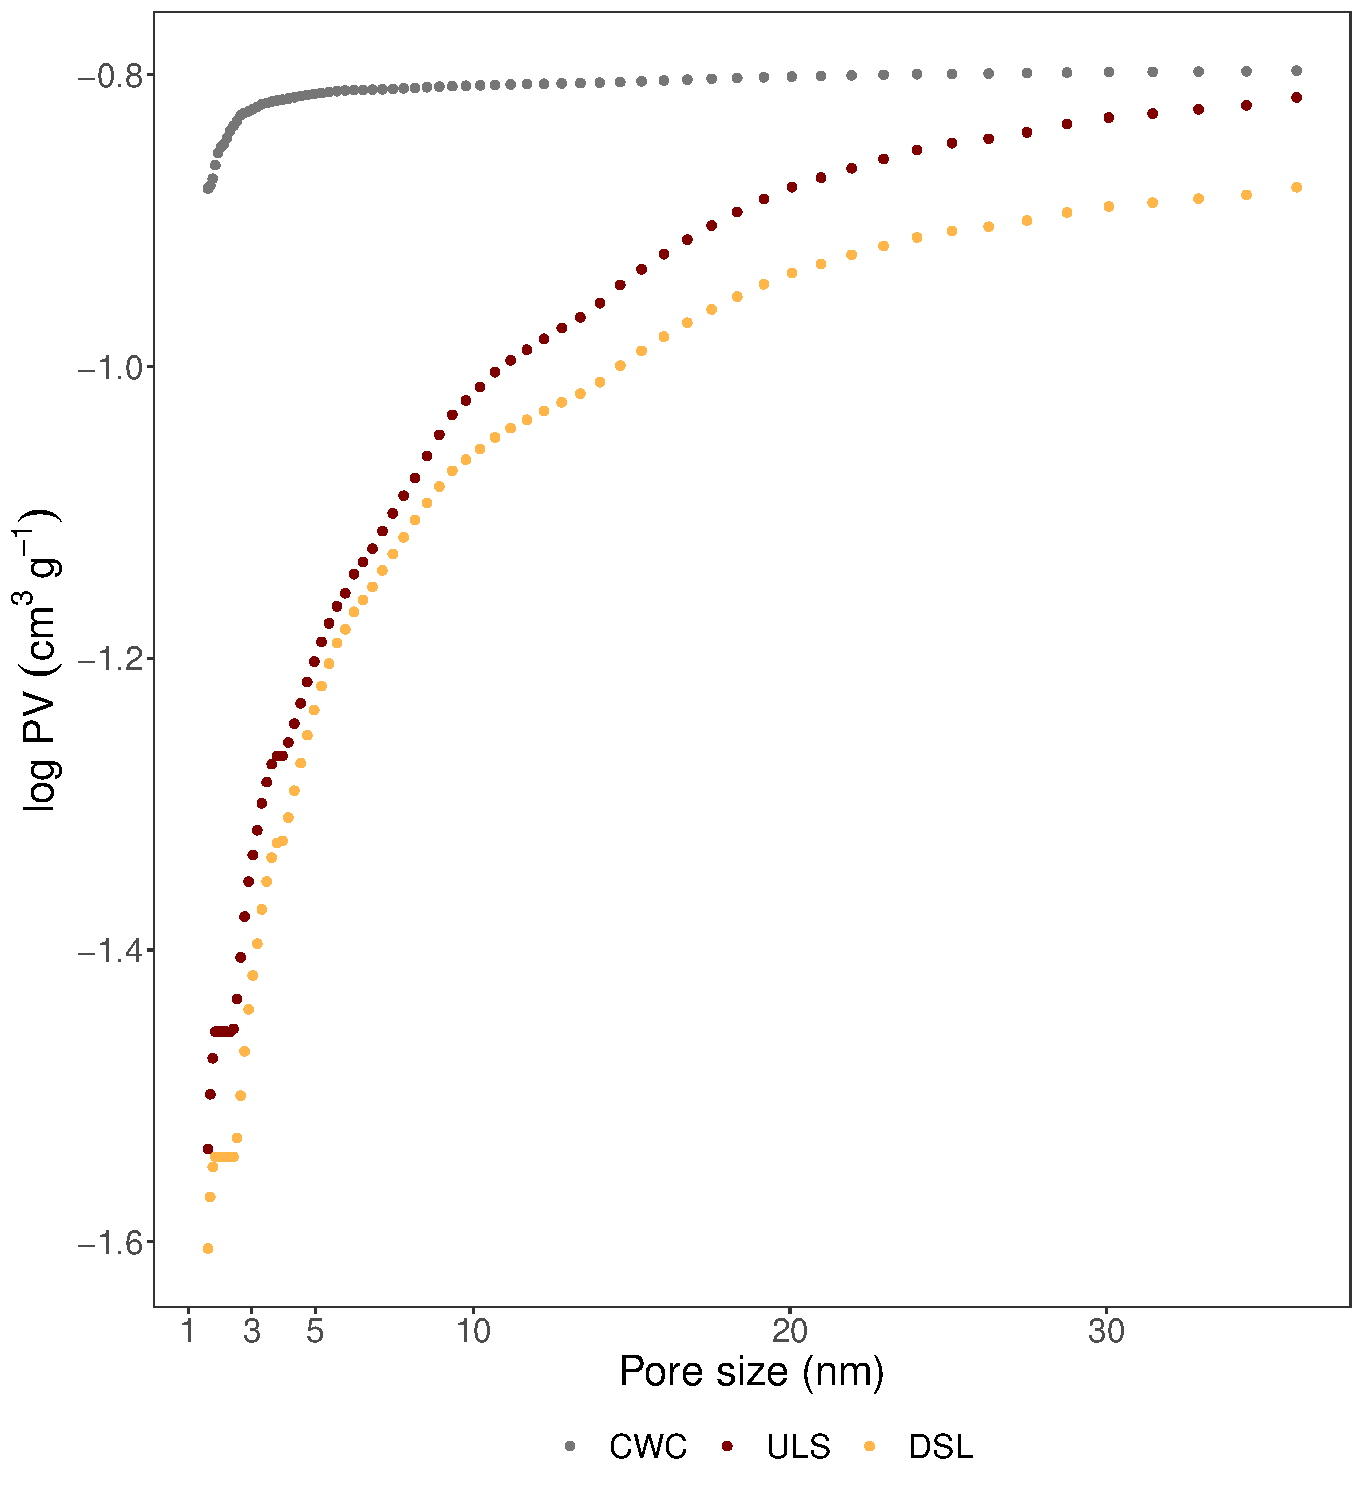
\includegraphics[width=0.45\textwidth]{R/figs/PV_large.pdf}
}
\hfill
\subfloat[\label{subfig:SAPV_large}]{%
  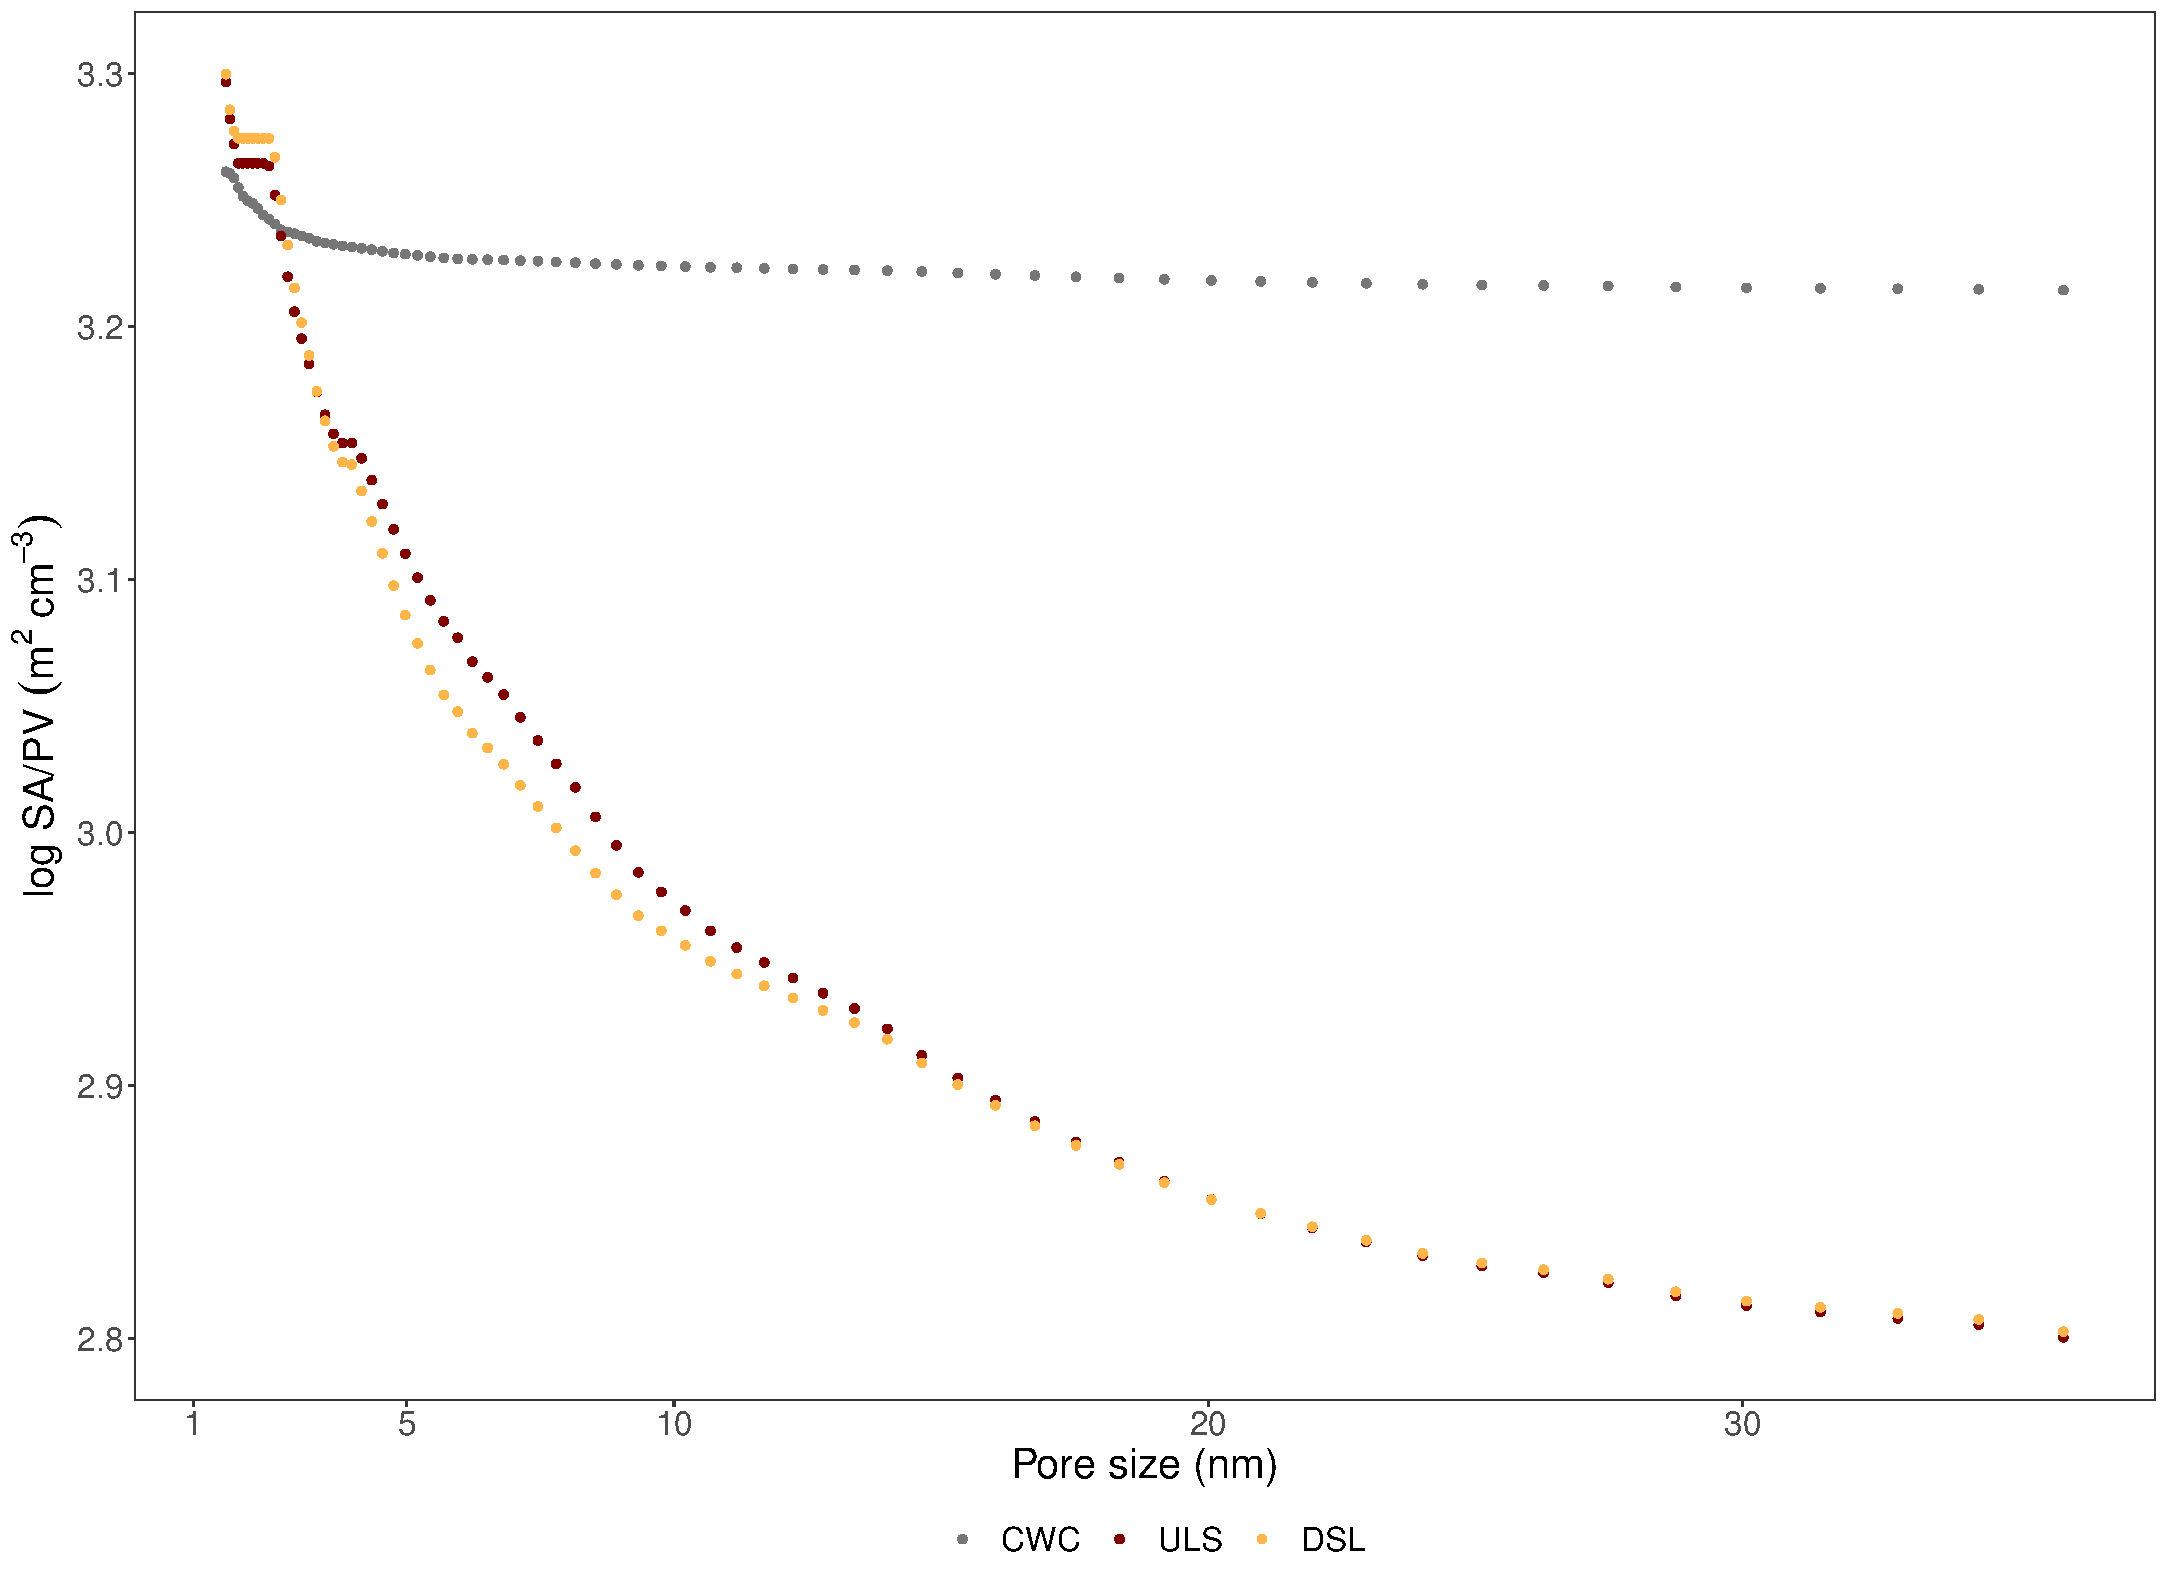
\includegraphics[width=0.45\textwidth]{R/figs/SAPV_large.pdf}
}
\hfill
\subfloat[\label{subfig:SAPV_C_large}]{%
  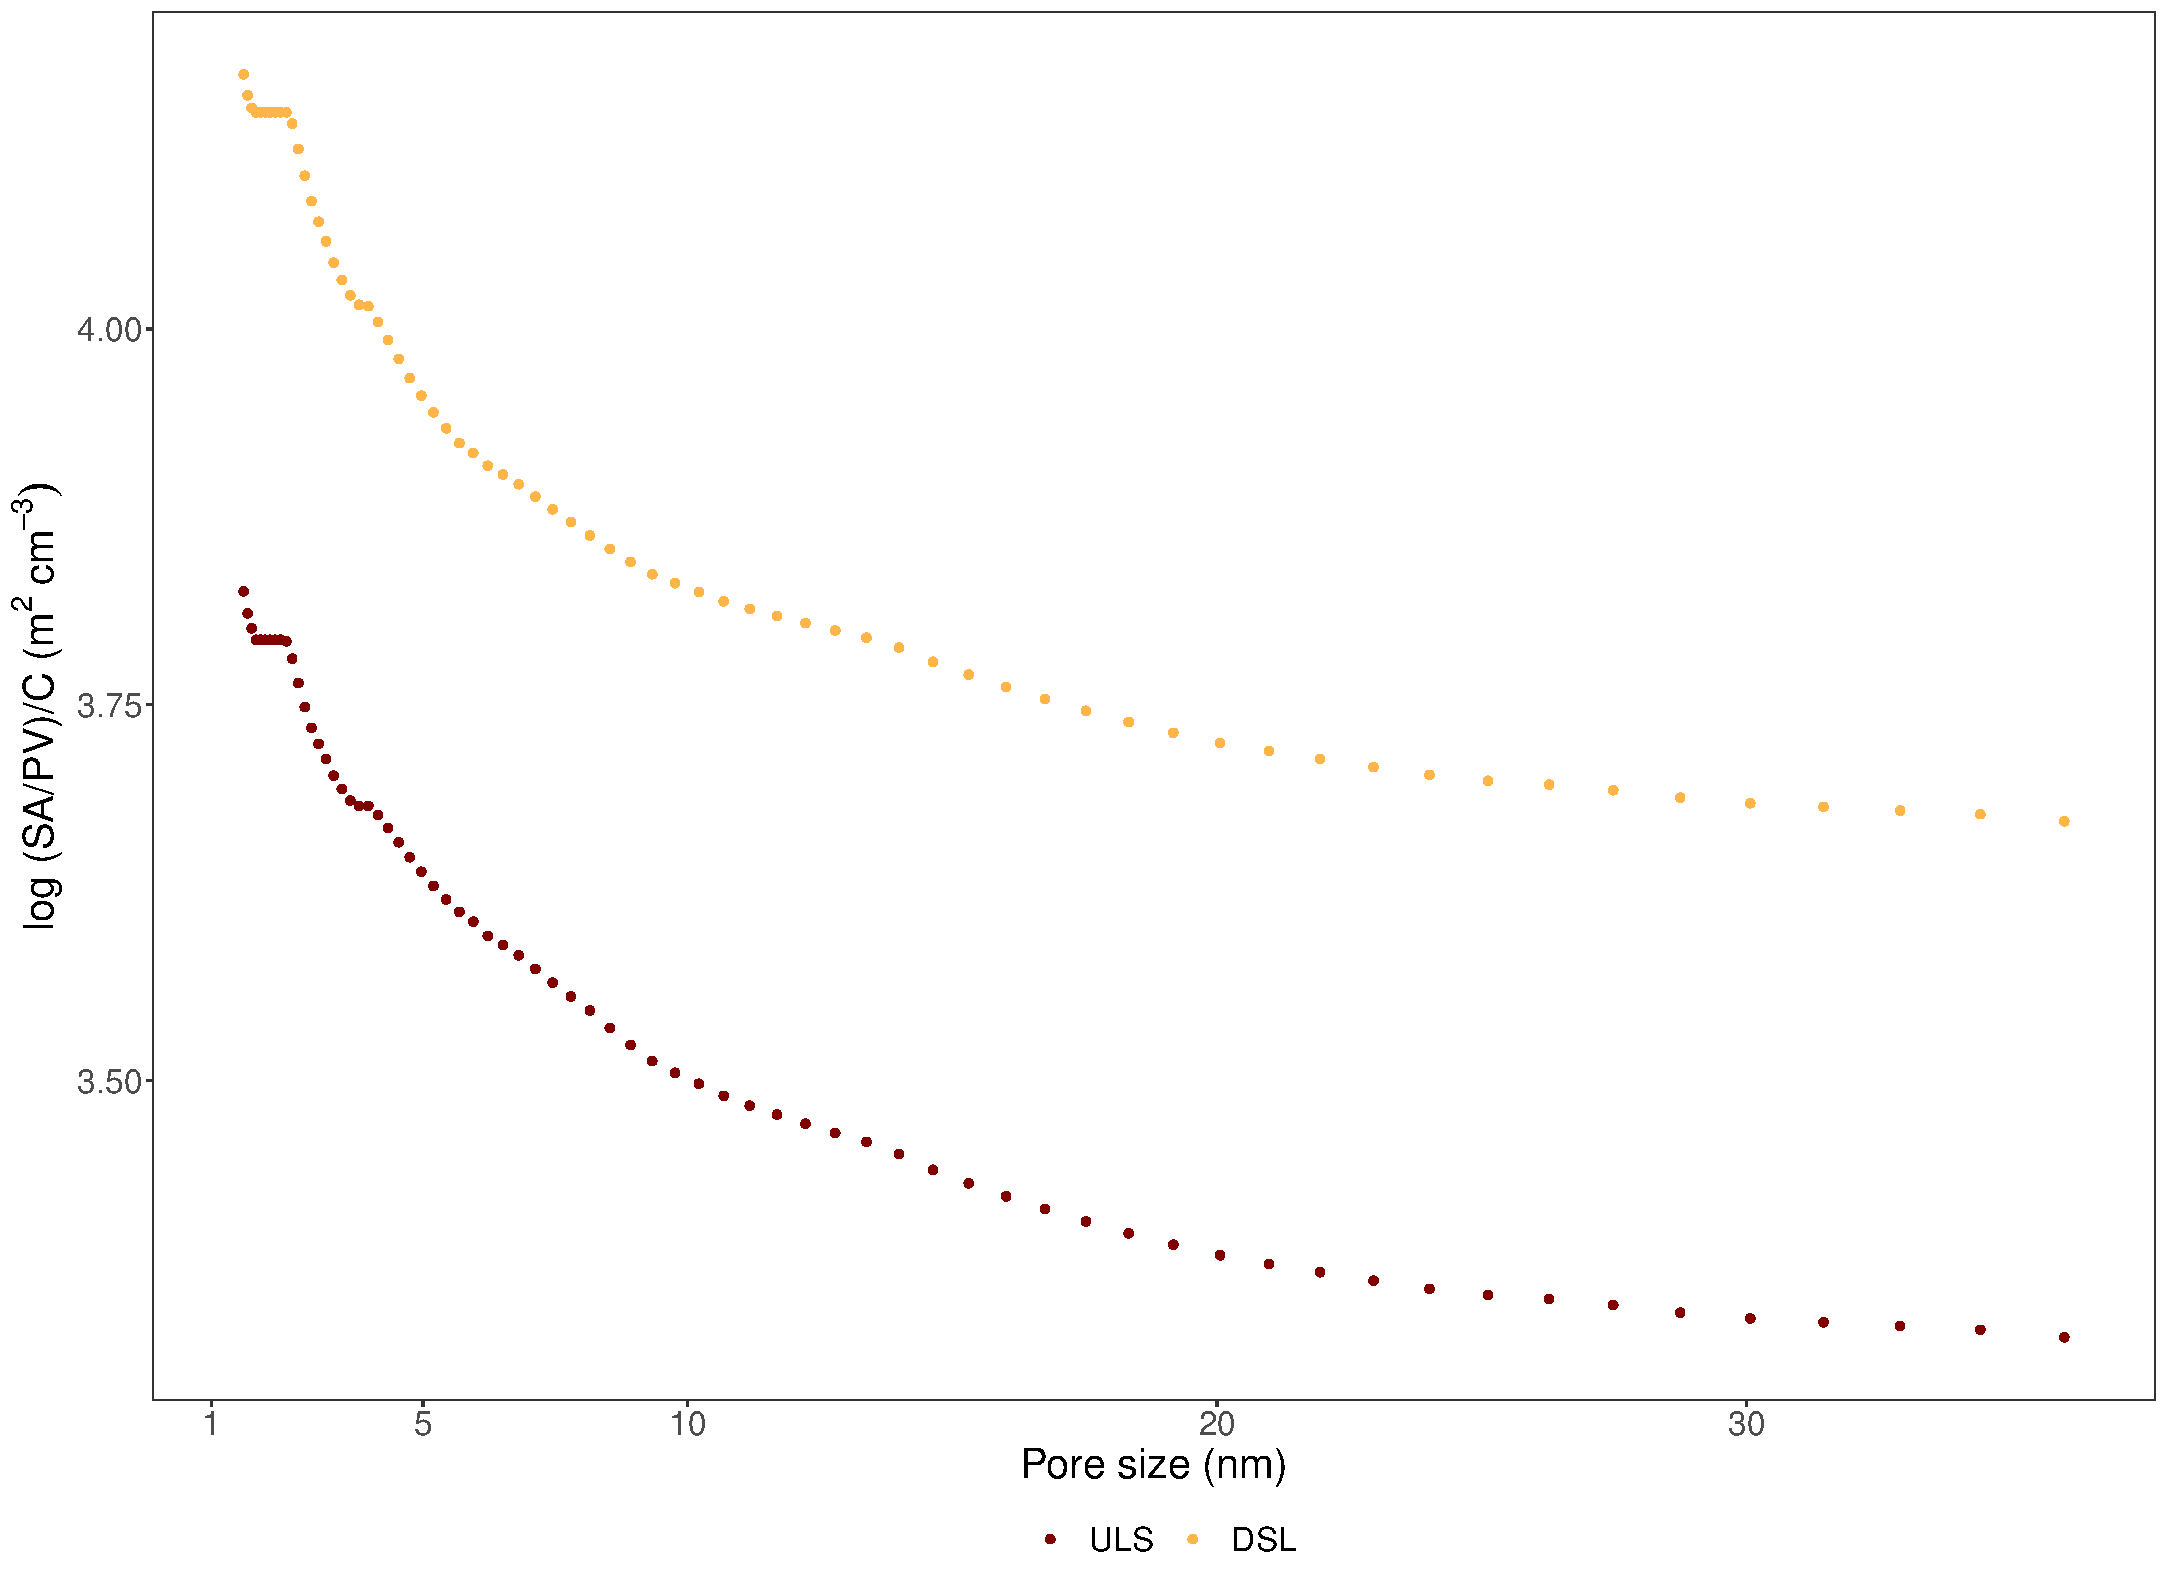
\includegraphics[width=0.45\textwidth]{R/figs/SAPV_C_large.pdf}
}
\caption{Cumulative pore size distribution for pores $>$ 1.5 nm using DFT theory. (a) Surface area, (b) pore volume, (c) SA/PV ratio for pores $>$1.5 nm normalized to carbon content (g C g BC\textsuperscript{-1}). (d) A lower SA/PV/C ratio indicates a higher degree of C in the pore wall matrix.}
\label{fig:PZD_large}
\end{figure}


\citep{yin2022insights,du2014adsorption} effects of salinity on sorption, states sorption increases with increasing salinity because the solubility of PFAS declines when the solution increases in ionic strength, making more PFCs separated from bulk solution onto adsorbents, which is called salting-out effect . 

\begin{figure}
    \centering
        \begin{subfigure}[]{\linewidth}
            \centering
            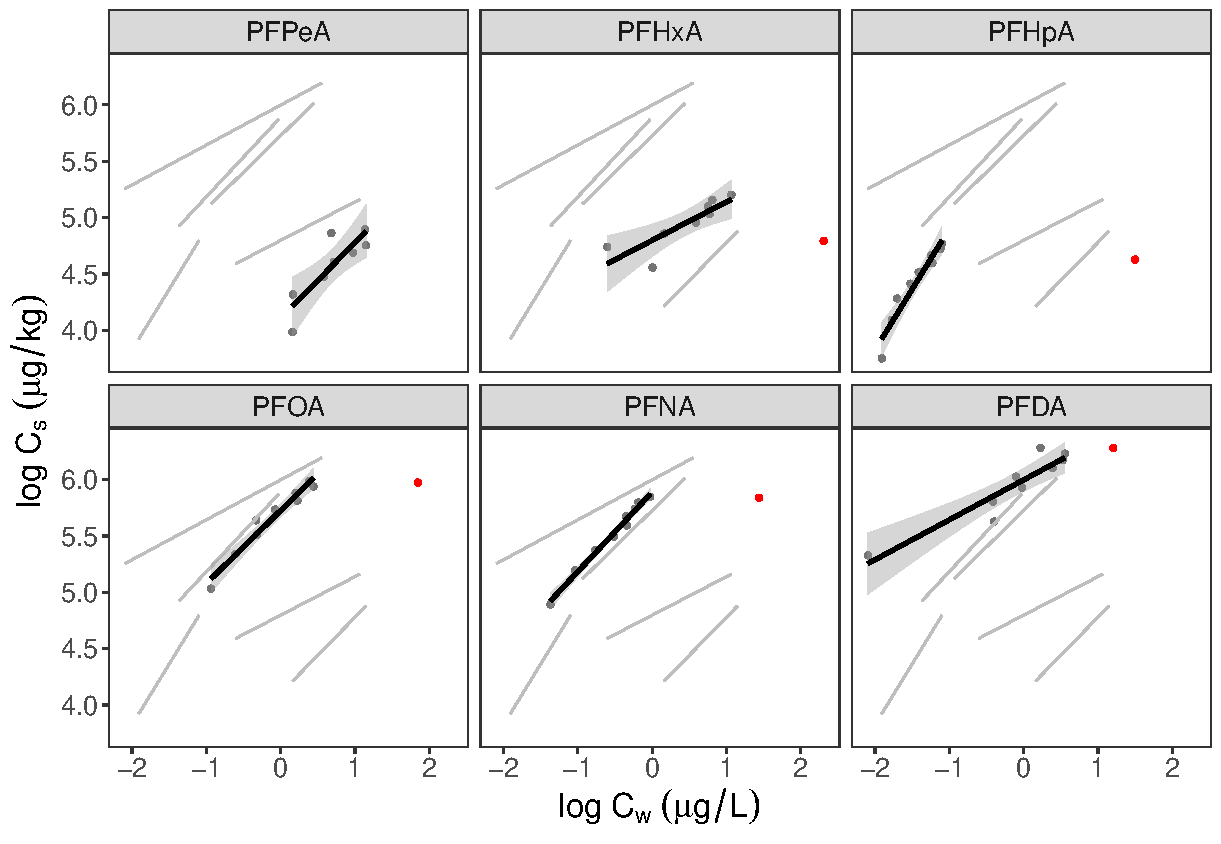
\includegraphics[width=0.6\textwidth]{R/figs/ULS_facet_isotherm.pdf}
            \subcaption{ULS isotherms}
            \label{fig:ULS_isotherm}
        \end{subfigure}
        \begin{subfigure}[]{\linewidth}
            \centering
            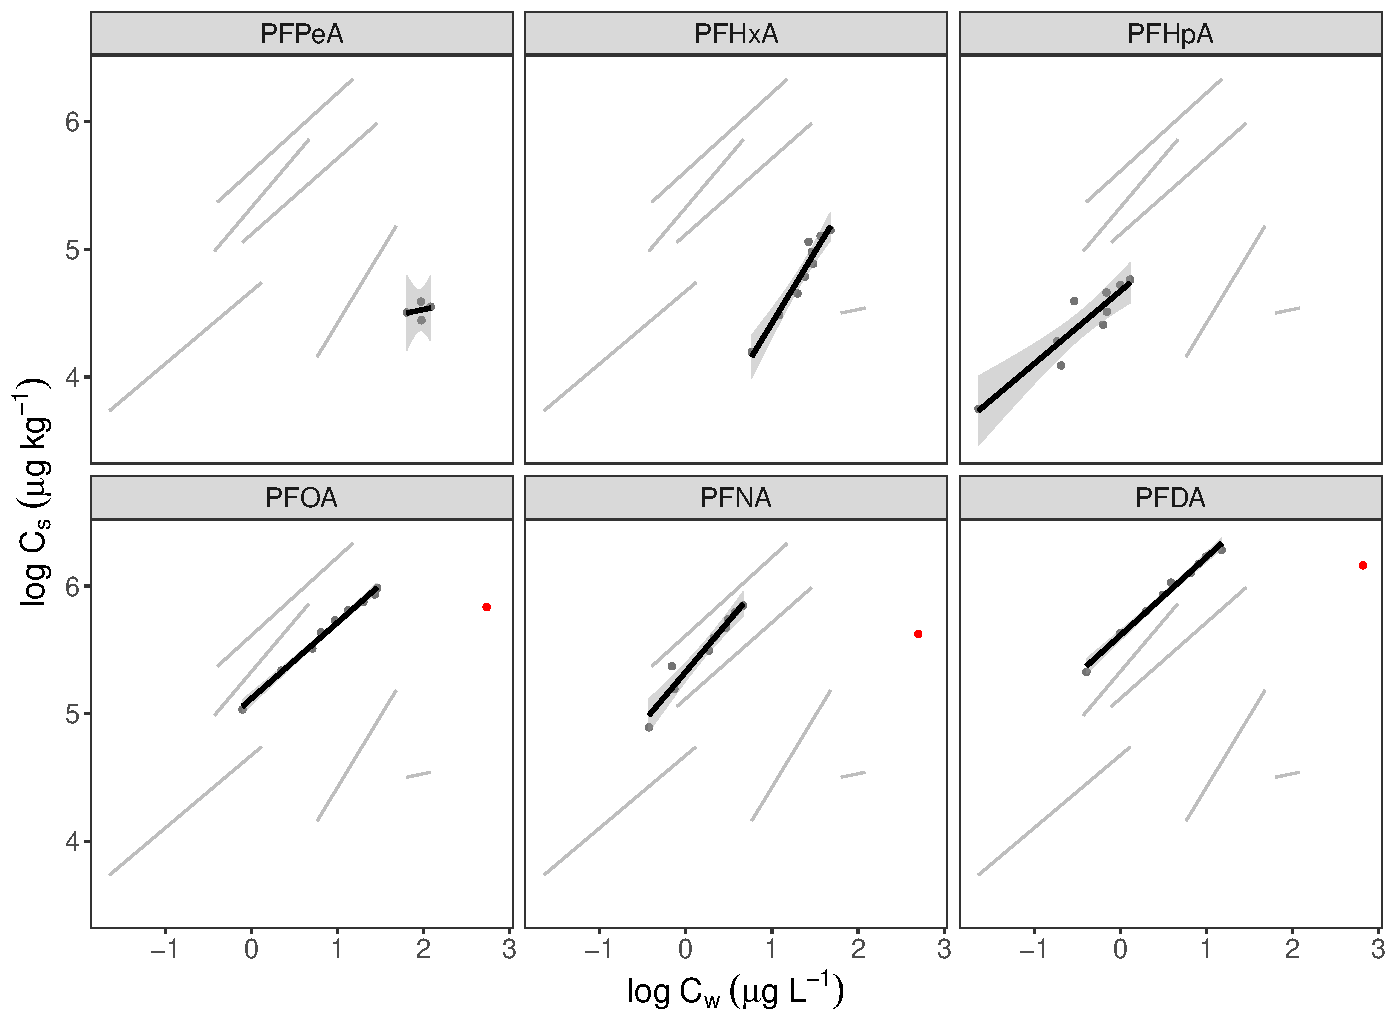
\includegraphics[width=0.6\textwidth]{R/figs/DSL_facet_isotherm.pdf}
            \subcaption{DSL isotherms}
            \label{fig:DSL_isotherm}
        \end{subfigure}   
\end{figure}
\begin{figure}[t]\ContinuedFloat
        \begin{subfigure}[]{\linewidth}
            \centering
            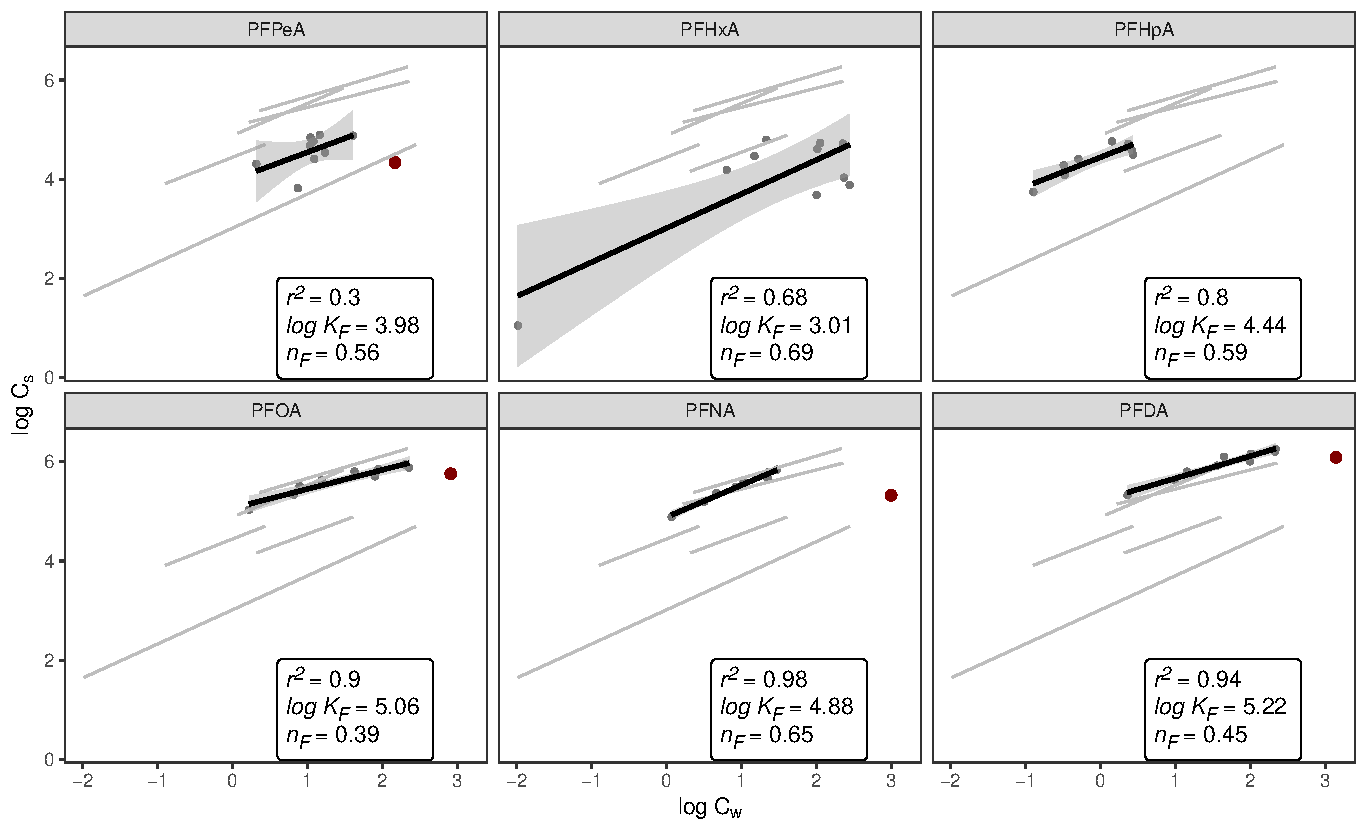
\includegraphics[width=0.6\textwidth]{R/figs/CWC_facet_isotherm.pdf}
            \subcaption{CWC isotherms}
            \label{fig:CWC_isotherm}
        \end{subfigure}
        \caption{Single-compound Freundlich sorption isotherms of PFPeA, PFHxA, PFHpA, PFOA, PFNA and PFDA. Lines are obtained by linear regression. For comparison across chain length, the shaded gray lines are the isotherms from the other compounds.}
        \label{fig:sorption_isotherms_all}
\end{figure}

%Consider removing this table
\begin{table}
\centering
\caption{Competition factor at SC10 (\cref{tab:spikeConcentrations}) for each compound and biochar. Competition factor is defined as K\textsubscript{d,single}/K\textsubscript{d,mix})$\times$100\%.}
\begin{threeparttable}
\label{tab:competition}
\begin{tabular}{lrrr}
\toprule
 & \multicolumn{3}{c}{Competition factor \%} \\ \cmidrule(l){2-4}
 & CWC & ULS & DSL \\ \midrule
PFPeA & 8.2 & \textsuperscript{*} & \textsuperscript{*} \\
PFHxA & \textsuperscript{*} & 2.3 & \textsuperscript{*} \\
PFHpA & \textsuperscript{*} & 0.2 & \textsuperscript{*} \\
PFOA & 15.8 & 3.4 & 4.4 \\
PFNA & 0.9 & 3.4 & 0.7 \\
PFDA & 10.6 & 10.9 & 3.1 \\ \bottomrule
\end{tabular}
\begin{tablenotes}
\item \textsuperscript{*} Amount in filtrate exceeded the amount spiked due to analytical uncertainty.
\end{tablenotes}
\end{threeparttable}
\end{table}

$K_d$ changes the least for PFHxA and PFHpA (2.3 and 0.2 \% respectively) and may be attributed to lower spiked concentrations (330 and 117 \textmu g L\textsuperscript{-1}) for these compounds compared to the rest in \cref{tab:competition}. Competition is most profound for PFOA to CWC followed by PFDA for ULS and CWC (15.8, 10.0 and 10.6 \% respectively), which can be explained by the highest concentrations spiked for these compounds (1 953 and 3 830 \textmu g L\textsuperscript{-1}). It appears that sorption of PFNA is minimally influenced by competition between other compounds despite SC being in the higher range (1 409 \textmu g L\textsuperscript{-1}). $K_d$ for PFPeA is reduced by 8.2\% and is expected based on weaker sorption of short-chain compounds.

\begin{figure}[htb]
    \centering
    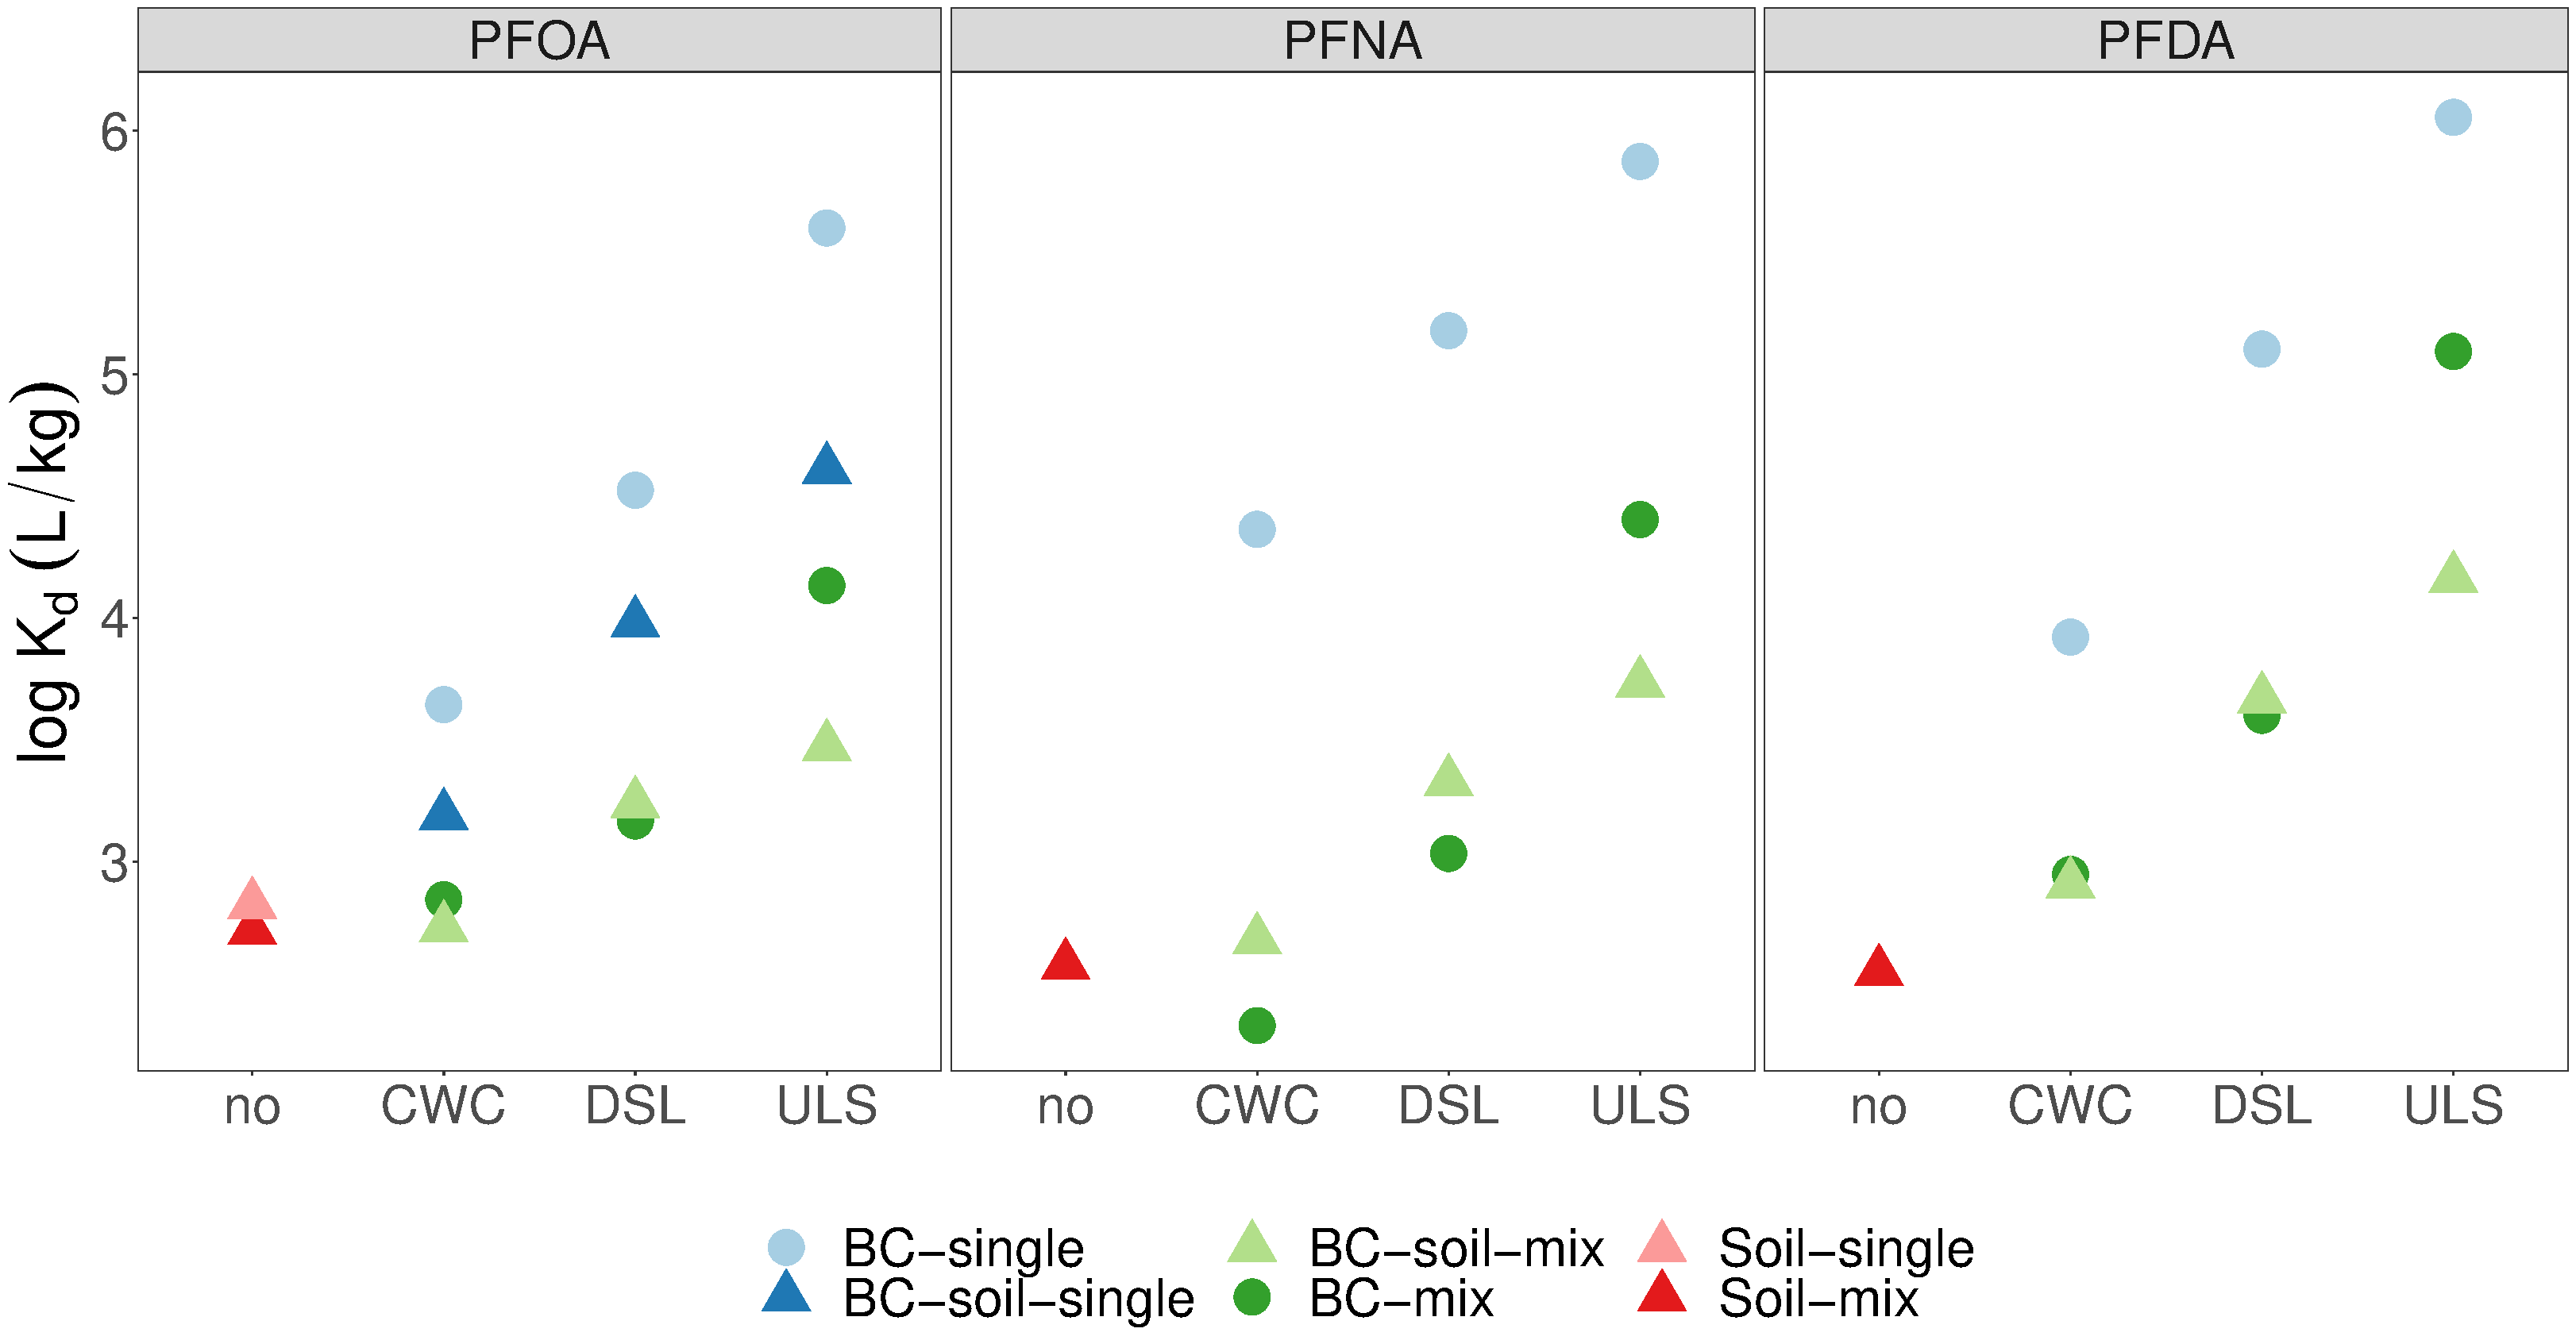
\includegraphics[width=0.8\textwidth]{R/figs/C10.pdf}
    \caption{Sorption attenuation for each TC by soil and/or competing congeners at SC10 (191, 330, 117, 1 953, 1 409, and 3 830 \textmu g L\textsuperscript{-1} for C5-C10, respectively). The error bars represent the standard deviation of $log~K_d$ for the cocktail batch tests performed in triplicate (not included). The single-compound $log~K_d$'s are single points.}
    \label{fig:C10}
\end{figure}
\begin{figure}[htb]
    \centering
    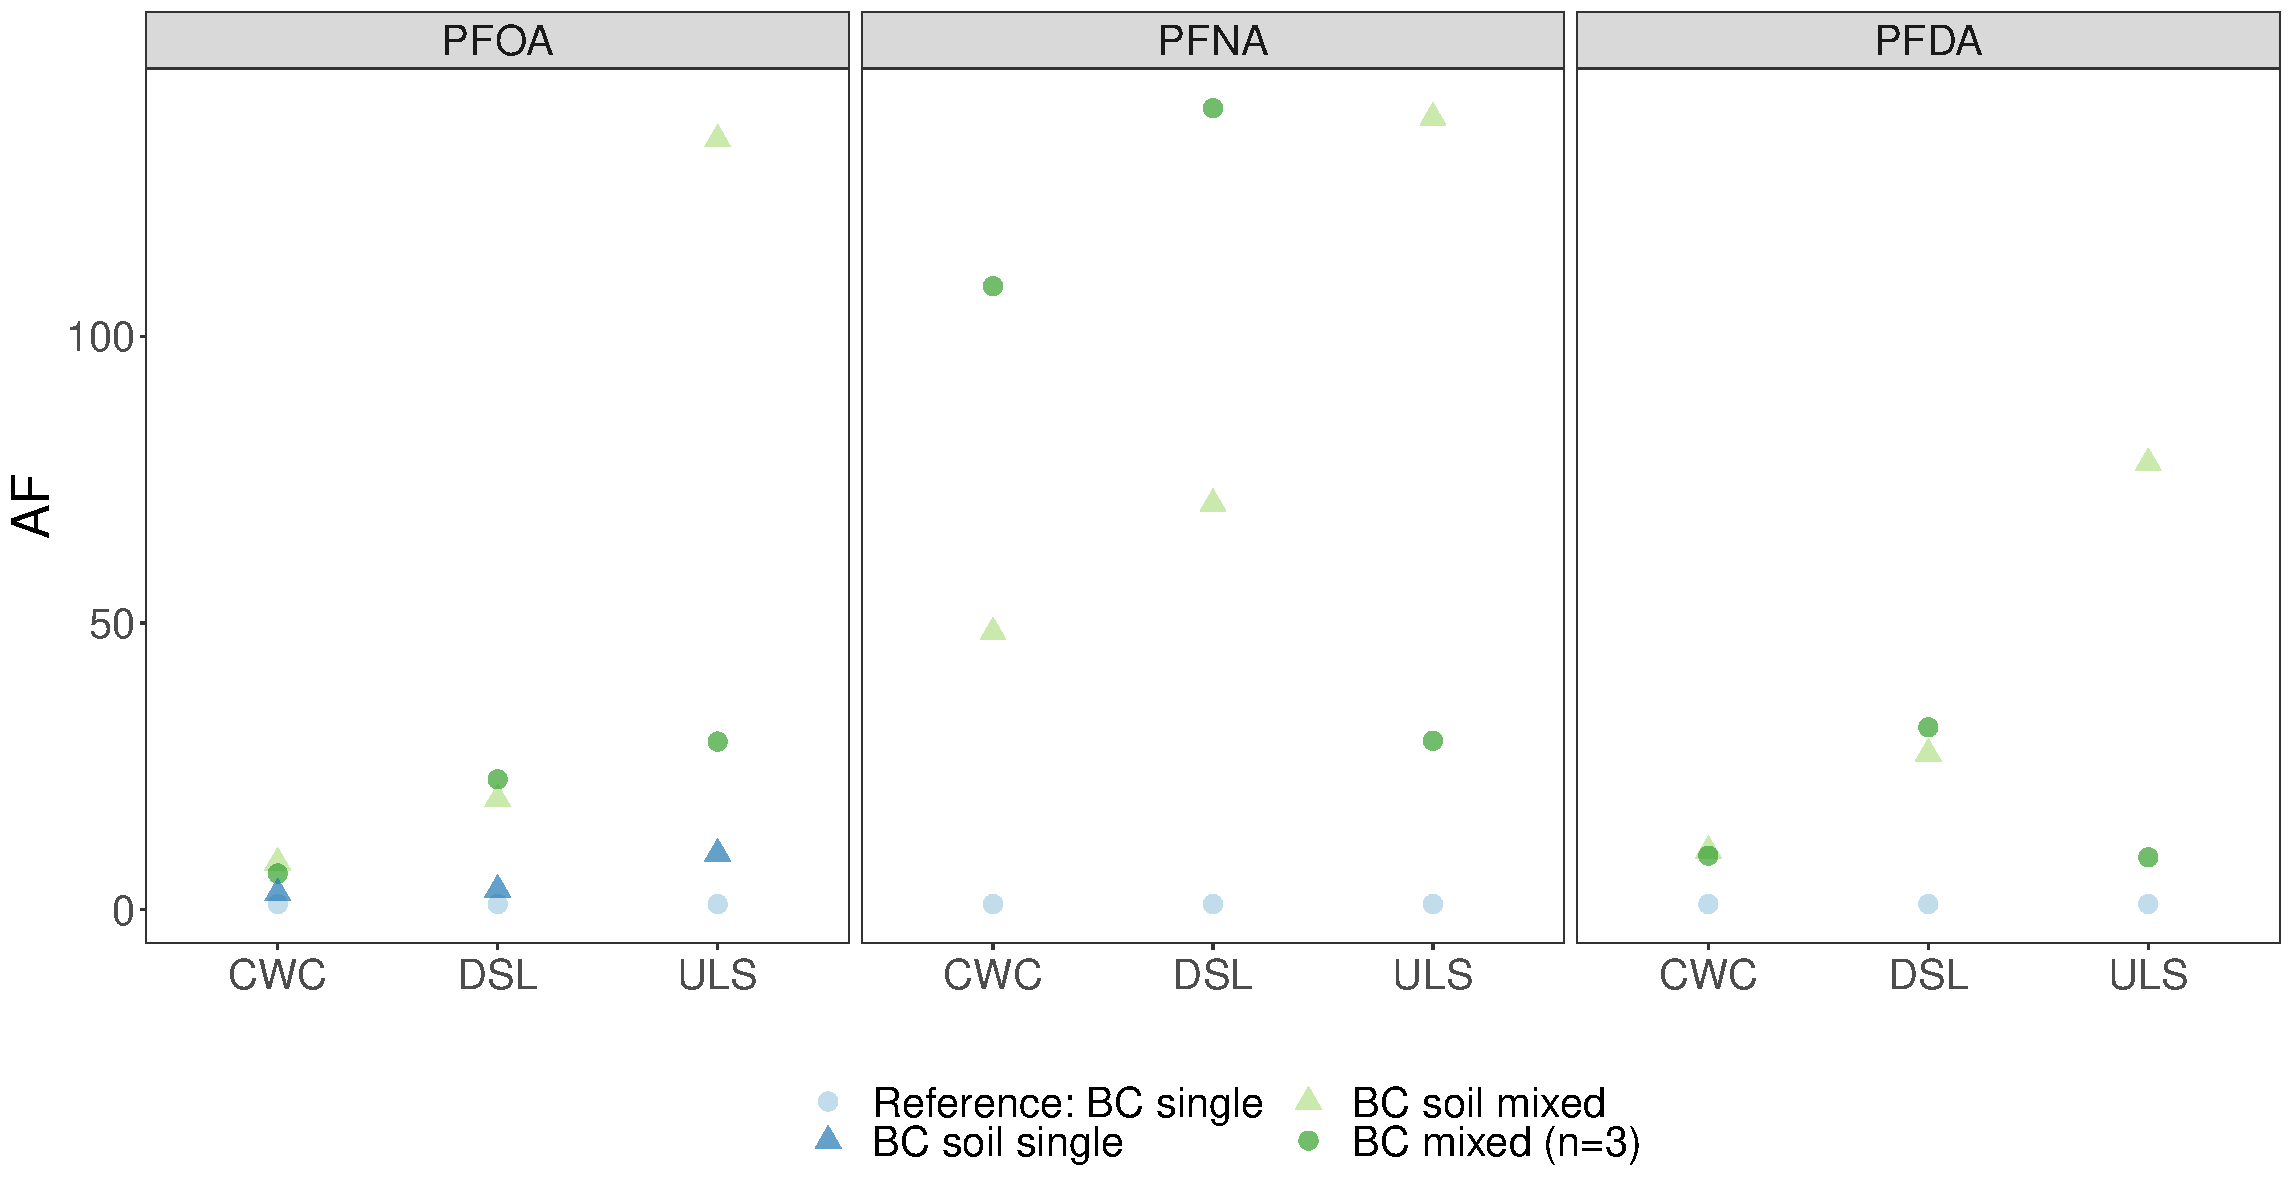
\includegraphics[width=0.8\textwidth]{R/figs/Attenuation_factors_C10_OND.pdf}
    \caption{Attenuation factors at C10 for C8-C10 calculated as \% reduction in $K_d$ from BC single. BC cocktails are spiked with 7.8 mg/L total PFCA and BC soil cocktails with 10.8 mg/L (the difference is due to analytical uncertainty and will be discussed assuming the that the spike concentrations are similar). See \cref{tab:spikeConcentrations} for spike concentrations used for each PFCA in the single-spike and cocktail-spike batch tests.}
    \label{fig:attenuation_factors}
\end{figure}

Attenuation: sorption decreases with time

Make figure showing different sorption mechanisms.\citep{Li2019} is a good place to start. Sorption of PFAS increases with pyrolysis temperature because then porosity and surface area increases.  \textit{in situ} bioremediation vs \textit{ex situ} bioremediation methods, pros and cons of each